% Options for packages loaded elsewhere
% Options for packages loaded elsewhere
\PassOptionsToPackage{unicode}{hyperref}
\PassOptionsToPackage{hyphens}{url}
\PassOptionsToPackage{dvipsnames,svgnames,x11names}{xcolor}
%
\documentclass[
  letterpaper,
  DIV=11,
  numbers=noendperiod]{scrreprt}
\usepackage{xcolor}
\usepackage{amsmath,amssymb}
\setcounter{secnumdepth}{5}
\usepackage{iftex}
\ifPDFTeX
  \usepackage[T1]{fontenc}
  \usepackage[utf8]{inputenc}
  \usepackage{textcomp} % provide euro and other symbols
\else % if luatex or xetex
  \usepackage{unicode-math} % this also loads fontspec
  \defaultfontfeatures{Scale=MatchLowercase}
  \defaultfontfeatures[\rmfamily]{Ligatures=TeX,Scale=1}
\fi
\usepackage{lmodern}
\ifPDFTeX\else
  % xetex/luatex font selection
\fi
% Use upquote if available, for straight quotes in verbatim environments
\IfFileExists{upquote.sty}{\usepackage{upquote}}{}
\IfFileExists{microtype.sty}{% use microtype if available
  \usepackage[]{microtype}
  \UseMicrotypeSet[protrusion]{basicmath} % disable protrusion for tt fonts
}{}
\makeatletter
\@ifundefined{KOMAClassName}{% if non-KOMA class
  \IfFileExists{parskip.sty}{%
    \usepackage{parskip}
  }{% else
    \setlength{\parindent}{0pt}
    \setlength{\parskip}{6pt plus 2pt minus 1pt}}
}{% if KOMA class
  \KOMAoptions{parskip=half}}
\makeatother
% Make \paragraph and \subparagraph free-standing
\makeatletter
\ifx\paragraph\undefined\else
  \let\oldparagraph\paragraph
  \renewcommand{\paragraph}{
    \@ifstar
      \xxxParagraphStar
      \xxxParagraphNoStar
  }
  \newcommand{\xxxParagraphStar}[1]{\oldparagraph*{#1}\mbox{}}
  \newcommand{\xxxParagraphNoStar}[1]{\oldparagraph{#1}\mbox{}}
\fi
\ifx\subparagraph\undefined\else
  \let\oldsubparagraph\subparagraph
  \renewcommand{\subparagraph}{
    \@ifstar
      \xxxSubParagraphStar
      \xxxSubParagraphNoStar
  }
  \newcommand{\xxxSubParagraphStar}[1]{\oldsubparagraph*{#1}\mbox{}}
  \newcommand{\xxxSubParagraphNoStar}[1]{\oldsubparagraph{#1}\mbox{}}
\fi
\makeatother

\usepackage{color}
\usepackage{fancyvrb}
\newcommand{\VerbBar}{|}
\newcommand{\VERB}{\Verb[commandchars=\\\{\}]}
\DefineVerbatimEnvironment{Highlighting}{Verbatim}{commandchars=\\\{\}}
% Add ',fontsize=\small' for more characters per line
\usepackage{framed}
\definecolor{shadecolor}{RGB}{241,243,245}
\newenvironment{Shaded}{\begin{snugshade}}{\end{snugshade}}
\newcommand{\AlertTok}[1]{\textcolor[rgb]{0.68,0.00,0.00}{#1}}
\newcommand{\AnnotationTok}[1]{\textcolor[rgb]{0.37,0.37,0.37}{#1}}
\newcommand{\AttributeTok}[1]{\textcolor[rgb]{0.40,0.45,0.13}{#1}}
\newcommand{\BaseNTok}[1]{\textcolor[rgb]{0.68,0.00,0.00}{#1}}
\newcommand{\BuiltInTok}[1]{\textcolor[rgb]{0.00,0.23,0.31}{#1}}
\newcommand{\CharTok}[1]{\textcolor[rgb]{0.13,0.47,0.30}{#1}}
\newcommand{\CommentTok}[1]{\textcolor[rgb]{0.37,0.37,0.37}{#1}}
\newcommand{\CommentVarTok}[1]{\textcolor[rgb]{0.37,0.37,0.37}{\textit{#1}}}
\newcommand{\ConstantTok}[1]{\textcolor[rgb]{0.56,0.35,0.01}{#1}}
\newcommand{\ControlFlowTok}[1]{\textcolor[rgb]{0.00,0.23,0.31}{\textbf{#1}}}
\newcommand{\DataTypeTok}[1]{\textcolor[rgb]{0.68,0.00,0.00}{#1}}
\newcommand{\DecValTok}[1]{\textcolor[rgb]{0.68,0.00,0.00}{#1}}
\newcommand{\DocumentationTok}[1]{\textcolor[rgb]{0.37,0.37,0.37}{\textit{#1}}}
\newcommand{\ErrorTok}[1]{\textcolor[rgb]{0.68,0.00,0.00}{#1}}
\newcommand{\ExtensionTok}[1]{\textcolor[rgb]{0.00,0.23,0.31}{#1}}
\newcommand{\FloatTok}[1]{\textcolor[rgb]{0.68,0.00,0.00}{#1}}
\newcommand{\FunctionTok}[1]{\textcolor[rgb]{0.28,0.35,0.67}{#1}}
\newcommand{\ImportTok}[1]{\textcolor[rgb]{0.00,0.46,0.62}{#1}}
\newcommand{\InformationTok}[1]{\textcolor[rgb]{0.37,0.37,0.37}{#1}}
\newcommand{\KeywordTok}[1]{\textcolor[rgb]{0.00,0.23,0.31}{\textbf{#1}}}
\newcommand{\NormalTok}[1]{\textcolor[rgb]{0.00,0.23,0.31}{#1}}
\newcommand{\OperatorTok}[1]{\textcolor[rgb]{0.37,0.37,0.37}{#1}}
\newcommand{\OtherTok}[1]{\textcolor[rgb]{0.00,0.23,0.31}{#1}}
\newcommand{\PreprocessorTok}[1]{\textcolor[rgb]{0.68,0.00,0.00}{#1}}
\newcommand{\RegionMarkerTok}[1]{\textcolor[rgb]{0.00,0.23,0.31}{#1}}
\newcommand{\SpecialCharTok}[1]{\textcolor[rgb]{0.37,0.37,0.37}{#1}}
\newcommand{\SpecialStringTok}[1]{\textcolor[rgb]{0.13,0.47,0.30}{#1}}
\newcommand{\StringTok}[1]{\textcolor[rgb]{0.13,0.47,0.30}{#1}}
\newcommand{\VariableTok}[1]{\textcolor[rgb]{0.07,0.07,0.07}{#1}}
\newcommand{\VerbatimStringTok}[1]{\textcolor[rgb]{0.13,0.47,0.30}{#1}}
\newcommand{\WarningTok}[1]{\textcolor[rgb]{0.37,0.37,0.37}{\textit{#1}}}

\usepackage{longtable,booktabs,array}
\usepackage{calc} % for calculating minipage widths
% Correct order of tables after \paragraph or \subparagraph
\usepackage{etoolbox}
\makeatletter
\patchcmd\longtable{\par}{\if@noskipsec\mbox{}\fi\par}{}{}
\makeatother
% Allow footnotes in longtable head/foot
\IfFileExists{footnotehyper.sty}{\usepackage{footnotehyper}}{\usepackage{footnote}}
\makesavenoteenv{longtable}
\usepackage{graphicx}
\makeatletter
\newsavebox\pandoc@box
\newcommand*\pandocbounded[1]{% scales image to fit in text height/width
  \sbox\pandoc@box{#1}%
  \Gscale@div\@tempa{\textheight}{\dimexpr\ht\pandoc@box+\dp\pandoc@box\relax}%
  \Gscale@div\@tempb{\linewidth}{\wd\pandoc@box}%
  \ifdim\@tempb\p@<\@tempa\p@\let\@tempa\@tempb\fi% select the smaller of both
  \ifdim\@tempa\p@<\p@\scalebox{\@tempa}{\usebox\pandoc@box}%
  \else\usebox{\pandoc@box}%
  \fi%
}
% Set default figure placement to htbp
\def\fps@figure{htbp}
\makeatother

\ifLuaTeX
  \usepackage{luacolor}
  \usepackage[soul]{lua-ul}
\else
  \usepackage{soul}
\fi




\setlength{\emergencystretch}{3em} % prevent overfull lines

\providecommand{\tightlist}{%
  \setlength{\itemsep}{0pt}\setlength{\parskip}{0pt}}



 
\usepackage[]{natbib}
\bibliographystyle{plainnat}


\usepackage{booktabs}
\KOMAoption{captions}{tableheading}
\makeatletter
\@ifpackageloaded{bookmark}{}{\usepackage{bookmark}}
\makeatother
\makeatletter
\@ifpackageloaded{caption}{}{\usepackage{caption}}
\AtBeginDocument{%
\ifdefined\contentsname
  \renewcommand*\contentsname{Table of contents}
\else
  \newcommand\contentsname{Table of contents}
\fi
\ifdefined\listfigurename
  \renewcommand*\listfigurename{List of Figures}
\else
  \newcommand\listfigurename{List of Figures}
\fi
\ifdefined\listtablename
  \renewcommand*\listtablename{List of Tables}
\else
  \newcommand\listtablename{List of Tables}
\fi
\ifdefined\figurename
  \renewcommand*\figurename{Figure}
\else
  \newcommand\figurename{Figure}
\fi
\ifdefined\tablename
  \renewcommand*\tablename{Table}
\else
  \newcommand\tablename{Table}
\fi
}
\@ifpackageloaded{float}{}{\usepackage{float}}
\floatstyle{ruled}
\@ifundefined{c@chapter}{\newfloat{codelisting}{h}{lop}}{\newfloat{codelisting}{h}{lop}[chapter]}
\floatname{codelisting}{Listing}
\newcommand*\listoflistings{\listof{codelisting}{List of Listings}}
\makeatother
\makeatletter
\makeatother
\makeatletter
\@ifpackageloaded{caption}{}{\usepackage{caption}}
\@ifpackageloaded{subcaption}{}{\usepackage{subcaption}}
\makeatother
\usepackage{bookmark}
\IfFileExists{xurl.sty}{\usepackage{xurl}}{} % add URL line breaks if available
\urlstyle{same}
\hypersetup{
  pdftitle={A Little R Survival Kit},
  pdfauthor={Eric S. Ho, Ph.D.},
  colorlinks=true,
  linkcolor={blue},
  filecolor={Maroon},
  citecolor={Blue},
  urlcolor={Blue},
  pdfcreator={LaTeX via pandoc}}


\title{A Little R Survival Kit}
\author{Eric S. Ho, Ph.D.}
\date{2026-06-16}
\begin{document}
\maketitle

\renewcommand*\contentsname{Table of contents}
{
\hypersetup{linkcolor=}
\setcounter{tocdepth}{2}
\tableofcontents
}

\bookmarksetup{startatroot}

\chapter*{Preface}\label{preface}
\addcontentsline{toc}{chapter}{Preface}

\markboth{Preface}{Preface}

In the 21st century, nobody does statistics by pen and paper. Those
statistical tables found at the back of statistics textbooks belong in
the museum. Statistics you hear from the news and research are produced
by computers. This book uses R. You may ask why not using a spreadsheet,
such as Microsoft Excel or Google Sheets. While they are excellent tools
- easy to use, they have significant shortcomings. In particular, they
lack of reproducibility, as they operate through point-clicking,
drag-and-drop, etc.

This book intends to provide readers with the bare minimum of R to start
analyzing data. In particular, this book is written for readers who have
scant experience in computer programming or scripting. I want them to
focus on deploying R's rich library of statistical tools to get the
desired results rather than being bogged down by the technical details
and cryptic syntax of the R language. Although most people think a book
like this is about R programming, I prefer to call it
\textbf{scripting}. The nuance is that the goal of programming is to
implement algorithms - a step-by-step procedure to tackle a problem like
a cooking recipe. Here we focus on what (expected results) instead of
how (algorithms); just tells the R functions here is the data and the
parameters, please process them and return the results.

\section*{Usage}\label{usage}
\addcontentsline{toc}{section}{Usage}

\markright{Usage}

The book consists of two parts. Part I focuses on the basics. Chapter 1
discusses R objects and operations act on these objects, including
descriptive statistical functions. Chapter 2 deals with data wrangling -
the process of acquiring, selecting, and organizing data stored in a
spreadsheet-like format. Both base R and \texttt{tidyverse} data
wrangling functions will be discussed. Part I is concluded with data
visualization in Chapter 3. A picture is worth a thousand words. The
chapter offers guidelines for choosing the most suitable graph according
to the intended message and properties of data. Both base R and
\texttt{ggplot2} graphical systems will be discussed. Part II covers
common statistical tests in Chapter 4. For readers who want to dive
deeper into intermediate R functions, Chapter 5 discusses R functions
that create or import data sets from files, restructure data sets, and
accelerate execution time.

\section*{RStudio}\label{rstudio}
\addcontentsline{toc}{section}{RStudio}

\markright{RStudio}

Scripting is best learned through hands-on practice; it is like learning
to swim. You don't just listen to lectures. You've got to jump into the
water and get wet! To try out the examples and exercises, you need to
use RStudio. There are two options to gain access to RStudio: cloud
service (Posit Cloud) and installing RStudio on your own computers. For
the first option, no software installation is required. All you need is
a Web Browser with Internet connection. For the first time, you can sign
up for an account and choose the plan from
\href{https://posit.cloud/plans?utm_source=Website&utm_medium=IDE_Download}{Posit
Cloud}. As this book covers the foundational R features, the basic, free
plan will work. Your work will be saved in the cloud under your account,
regardless what computer you use, as long as you log in to the same
account.

Alternatively, if you prefer to have a better control of RStudio, you
can install R and RStudio on your own computers. However, it becomes
your responsibility to maintain and update them in the future. Why do
you need to install two programs instead of just RStudio? In a car
analogy, R is like the engine, and RStudio is like the dashboard.
RStudio provides a user-friendly Interactive Development Environment
(IDE) for users to instruct R to perform the actual work. A favorable
feature of R is that it can be installed on a Windows or a Mac computer.
If your computer is a Chromebook, Posit Cloud is a preferred, as the
installation of R and RStudio on a Chromebook is less straightforward.
For Windows and Mac, the installation is simple; it only takes a few
double-clicks. Note that you must install R before RStudio. Here are the
links to download \href{https://cran.r-project.org/}{R} and
\href{https://posit.co/download/rstudio-desktop/}{RStudio}.

Lastly, this is a live book that I will continue to update with topics
to help readers like you. I invite you to check back periodically to
discover new material.

\part{Part I}

\chapter{Basic R}\label{sec-01-basic-r}

\section*{Learning Objectives:}\label{learning-objectives}
\addcontentsline{toc}{section}{Learning Objectives:}

\markright{Learning Objectives:}

The journey of R scripting starts with a basic understanding of R
objects and commands. After finishing this chapter, you should be able
to:

\begin{itemize}
\item
  Define R variables.
\item
  Know the differences between an atomic variable and an object
  variable.
\item
  Store results in variables through the assignment operator.
\item
  Perform arithmetic operations.
\item
  Handle composite objects: vectors and data frames.
\item
  Define categorical variables.
\item
  Calculate descriptive and summary statistics.
\item
  Utilize inspection functions to figure out basic information about
  data.
\item
  Format and print the contents of variables to the console.
\item
  Use \texttt{seq()} and \texttt{with()} functions.
\end{itemize}

As R scripting is a hands-on topic, I encourage you to open RStudio
alongside this book and try out the code to maximize understanding.
Let's get started.

\section{R Variables}\label{r-variables}

An R variable is a named location in the computer's memory that stores
some values. Imagine it as a labeled (name) shoebox (memory location)
keeping a pair of sneakers (value).

Two rules determine how an R variable can be named:

\begin{enumerate}
\def\labelenumi{\arabic{enumi}.}
\item
  It must begin with a letter (A-Z or a-z), a dot ``\texttt{.}'', or an
  underscore ``\texttt{\_}'', and
\item
  Subsequent characters can be any combination of letters, digits (0-9),
  ``\texttt{.}'', or ``\texttt{\_}''.
\end{enumerate}

Note that:

\begin{itemize}
\item
  A variable name can be as short as one character or as long as a
  normal person wishes (10,000 characters!).
\item
  My suggestion is to give variables meaningful names that help you or
  someone else comprehend the code. For instance, in a problem about
  heart rate, use \texttt{zone2} instead of \texttt{z} or even worse
  \texttt{x}.
\item
  Be careful that variable names are case-sensitive, e.g.,
  \texttt{volume} and \texttt{Volume} are different in the eyes of R.
\item
  Avoid naming variables with names that have been reserved by R
  (https://rdrr.io/r/base/Reserved.html) or names already used to name
  R's built-in functions, e.g., \texttt{c}, and \texttt{head}. For the
  latter, unfortunately, R is permissive for misnaming variables by
  remaining silent, costing time to identify the issue. Therefore, the
  rule of thumb is to exercise self-discipline and avoid using R
  function names as variable names.
\end{itemize}

\section{R Objects}\label{r-objects}

Every variable is an R object. In scripting, it is important to know the
type(s) of value(s) being stored in a variable, as the types dictate the
legitimate operations that act on the variable. Let's begin with data
types.

\subsection{Data Types}\label{sec-data-types}

R supports six data types:

\begin{itemize}
\item
  Double: decimal numbers, e.g., 5.6, -4.3
\item
  Integer: whole numbers, e.g, -10, 56
\item
  Character: they contain text, e.g., ``ACGT'', ``Hello World''
\item
  Logical: \texttt{TRUE} or \texttt{FALSE}
\item
  Complex\textsuperscript{\texttt{*}}: Complex numbers containing real
  and imaginary components, e.g., 5+2i
\item
  Raw\textsuperscript{\texttt{*}}: Bare bytes of data.
\end{itemize}

\texttt{*} We will only discuss the first four types in this book; you
can ignore complex and raw types.

\subsection{Atomic and Composite
Variables}\label{sec-atomic-and-composite-variables}

From a practical perspective, R variables can be viewed as
\textbf{atomic variables} and \textbf{composite variables}. An atomic
variable contains a single value, and a composite variable consists of a
collection of values. Let us begin with two atomic variables:
\textbf{\texttt{numeric}}, and \textbf{\texttt{character}}.

\subsubsection{Numeric Variables}\label{numeric-variables}

An atomic numeric variable holds a decimal number (\texttt{double}) or a
whole number (\texttt{integer}). Numbers can be represented in
scientific notation. Here are some examples:

\begin{Shaded}
\begin{Highlighting}[]
\CommentTok{\# Decimal}
\NormalTok{height }\OtherTok{\textless{}{-}} \FloatTok{5.6}

\CommentTok{\# Whole number (Integer)}
\NormalTok{sample\_size }\OtherTok{\textless{}{-}} \DecValTok{15}\NormalTok{L}

\CommentTok{\# Scientific notation}
\NormalTok{avogadro\_number }\OtherTok{\textless{}{-}} \FloatTok{6.023e23}
\end{Highlighting}
\end{Shaded}

\texttt{\textless{}-} is the assignment operator. It looks like a
left-pointing arrow, depicting the transfer of value from the right-hand
side to the left-hand side. Upon execution, the resultant value of the
expression on the right-hand side, if no error occurs, is stored in the
named variable on the left-hand side. In RStudio, you can see the
variable name and its associated value under the \textbf{Environment}
tab, which usually occupies the top right quadrant of the RStudio
desktop.

Note that R supports another assignment operator: \texttt{=}. You can
use \texttt{\textless{}-} and \texttt{=} interchangeably. I prefer
\texttt{\textless{}-} to \texttt{=}, as \texttt{=} can easily confuse
with the equality checking operator \texttt{==}.

A few words about the scientific notation. It comprises three parts: the
coefficient, a constant literal\texttt{e}, and the exponent. The
\texttt{e} refers to the base \texttt{10}. For example, the R's
scientific notation of \(6.023\times10^{23}\) is \texttt{6.023e23},
where the coefficient and the exponent are \(6.023\) and \(23\),
respectively. Note that you must not include spaces in scientific
notation, e.g., \texttt{6.023e\ 23}, \texttt{6.023\ e23}, or
\texttt{6.023\ e\ 23} will return errors.

\textbf{Arithmetic Operators}

You can apply arithmetic operations on numeric variables. Here are the
arithmetic operators: \texttt{+} (addition), \texttt{-} (subtraction),
\texttt{*} (multiplication), \texttt{/} (division), \texttt{**}
(exponentiation), and \texttt{\^{}} (exponentiation). The last two
exponentiation operators perform the same function. Here are some
examples:

\begin{Shaded}
\begin{Highlighting}[]
\NormalTok{radius }\OtherTok{\textless{}{-}} \FloatTok{2.5}
\NormalTok{diameter }\OtherTok{\textless{}{-}} \DecValTok{2}\SpecialCharTok{*}\NormalTok{pi}\SpecialCharTok{*}\NormalTok{radius}
\NormalTok{pi }\OtherTok{\textless{}{-}} \FloatTok{3.1416}
\NormalTok{area }\OtherTok{\textless{}{-}}\NormalTok{ pi}\SpecialCharTok{*}\NormalTok{radius}\SpecialCharTok{**}\DecValTok{2}
\NormalTok{volume }\OtherTok{\textless{}{-}}\NormalTok{ (}\DecValTok{4}\SpecialCharTok{/}\DecValTok{3}\NormalTok{)}\SpecialCharTok{*}\NormalTok{pi}\SpecialCharTok{*}\NormalTok{radius}\SpecialCharTok{\^{}}\DecValTok{3}
\end{Highlighting}
\end{Shaded}

\subsubsection{Character Variables}\label{character-variables}

R also supports text values, which are in \texttt{character} data type.
To define a character value, you need to use a pair of quotes to enclose
the text. Either a pair of single (\texttt{\textquotesingle{}}) or
double quotes (\texttt{"}) works. E.g.,

\begin{Shaded}
\begin{Highlighting}[]
\NormalTok{course }\OtherTok{\textless{}{-}} \StringTok{\textquotesingle{}BIOL265\textquotesingle{}}
\end{Highlighting}
\end{Shaded}

To figure out whether a variable's type is numeric, character, or
something else, use the \texttt{typeof()} function,

\begin{Shaded}
\begin{Highlighting}[]
\FunctionTok{typeof}\NormalTok{(course)}
\end{Highlighting}
\end{Shaded}

\begin{verbatim}
[1] "character"
\end{verbatim}

\begin{Shaded}
\begin{Highlighting}[]
\FunctionTok{typeof}\NormalTok{(area)}
\end{Highlighting}
\end{Shaded}

\begin{verbatim}
[1] "double"
\end{verbatim}

Obviously, it does not make sense to do math with character type. E.g.,

\begin{Shaded}
\begin{Highlighting}[]
\NormalTok{course}\SpecialCharTok{*}\DecValTok{4}
\end{Highlighting}
\end{Shaded}

\begin{verbatim}
Error in `course * 4`:
! non-numeric argument to binary operator
\end{verbatim}

You can use \texttt{nchar()} function to figure out the number of
characters, including spaces and punctuation, of a character variable.
E.g.,

\begin{Shaded}
\begin{Highlighting}[]
\FunctionTok{nchar}\NormalTok{(course)}
\end{Highlighting}
\end{Shaded}

\begin{verbatim}
[1] 7
\end{verbatim}

\subsection{Vectors}\label{sec-vectors}

One common composite variable in R is \textbf{\texttt{vectors}}. It is
an ordered sequence of items that can be processed collectively as a
whole, or individually. A vector can be viewed pictorially as a wagon
train in which carriages are coupled one after the other. E.g.,

\begin{Shaded}
\begin{Highlighting}[]
\CommentTok{\# A simple numeric vector for the days in each month}
\NormalTok{days\_of\_month }\OtherTok{\textless{}{-}} \FunctionTok{c}\NormalTok{(}\DecValTok{31}\NormalTok{, }\DecValTok{28}\NormalTok{, }\DecValTok{31}\NormalTok{, }\DecValTok{30}\NormalTok{, }\DecValTok{31}\NormalTok{, }\DecValTok{30}\NormalTok{, }\DecValTok{31}\NormalTok{, }\DecValTok{31}\NormalTok{, }\DecValTok{30}\NormalTok{, }\DecValTok{31}\NormalTok{, }\DecValTok{30}\NormalTok{, }\DecValTok{31}\NormalTok{)}
\end{Highlighting}
\end{Shaded}

\texttt{days\_of\_month} is a \texttt{vector} object in R.
\textbf{\texttt{c()}} is the function that \textbf{combines or collates}
several objects into a vector object. Items are indexed or numbered from
1 to the total number of items in the vector. You can extract a
particular item by specifying the index within a pair of
square-brackets. E.g.,

\begin{Shaded}
\begin{Highlighting}[]
\CommentTok{\# Days in February}
\FunctionTok{print}\NormalTok{(days\_of\_month[}\DecValTok{2}\NormalTok{])}
\end{Highlighting}
\end{Shaded}

\begin{verbatim}
[1] 28
\end{verbatim}

The \texttt{{[}2{]}} means the 2\textsuperscript{nd} element of a
vector. We will discuss indexing in more detail below.

Here is an example of a character vector:

\begin{Shaded}
\begin{Highlighting}[]
\NormalTok{nucleotides }\OtherTok{\textless{}{-}} \FunctionTok{c}\NormalTok{(}\StringTok{\textquotesingle{}A\textquotesingle{}}\NormalTok{,}\StringTok{\textquotesingle{}C\textquotesingle{}}\NormalTok{,}\StringTok{\textquotesingle{}G\textquotesingle{}}\NormalTok{,}\StringTok{\textquotesingle{}T\textquotesingle{}}\NormalTok{)}
\end{Highlighting}
\end{Shaded}

Noteworthy that all items held inside a vector must have the same data
type. In other words, vectors are always \textbf{homogeneous}. For
instance, \texttt{days\_of\_month} contains all numeric values, and
\texttt{nucleotides} contains all character values. If you try to
combine objects of different data types into a vector, R will
automatically convert them to character type, the lowest denominator of
data types. In the example below, even though the first and third values
are entered as numeric, R coerces them into text \texttt{"1"} and
\texttt{"0"}.

\begin{Shaded}
\begin{Highlighting}[]
\NormalTok{a\_vector }\OtherTok{\textless{}{-}} \FunctionTok{c}\NormalTok{(}\DecValTok{1}\NormalTok{, }\StringTok{"success"}\NormalTok{, }\DecValTok{0}\NormalTok{, }\StringTok{"fail"}\NormalTok{)}
\NormalTok{a\_vector}
\end{Highlighting}
\end{Shaded}

\begin{verbatim}
[1] "1"       "success" "0"       "fail"   
\end{verbatim}

One of the R features that makes arithmetic operations on vectors really
convenient is \textbf{vectorization}. For instance, if you want to
standardize the values of a sample such that the sample mean and sample
variance after standardization become 0 and 1, respectively. The formula
for standardization is \(z_{i}=\frac{(x_{i}-\bar{x})}{s}\), where
\(\bar{x}\) and \(s\) are the sample mean and sample standard deviation,
respectively. Here's an example

\begin{Shaded}
\begin{Highlighting}[]
\NormalTok{heights }\OtherTok{\textless{}{-}} \FunctionTok{c}\NormalTok{(}\FloatTok{5.5}\NormalTok{, }\FloatTok{6.0}\NormalTok{, }\FloatTok{6.1}\NormalTok{, }\FloatTok{5.7}\NormalTok{, }\FloatTok{5.9}\NormalTok{, }\FloatTok{5.6}\NormalTok{)}
\NormalTok{x\_bar }\OtherTok{\textless{}{-}} \FunctionTok{mean}\NormalTok{(heights)}
\NormalTok{s }\OtherTok{\textless{}{-}} \FunctionTok{sd}\NormalTok{(heights)}
\NormalTok{std\_heights }\OtherTok{\textless{}{-}}\NormalTok{ (heights }\SpecialCharTok{{-}}\NormalTok{ x\_bar)}\SpecialCharTok{/}\NormalTok{s}
\NormalTok{std\_heights}
\end{Highlighting}
\end{Shaded}

\begin{verbatim}
[1] -1.2677314  0.8451543  1.2677314 -0.4225771  0.4225771 -0.8451543
\end{verbatim}

\texttt{mean()} and \texttt{sd()} are built-in functions that calculate
the average and standard deviation of a sample, respectively.

The convenience is that you don't have to specify how to subtract and
divide each height individually. Instead, R recognizes the expression
\texttt{(heights-x\_bar)} is to subtract an atomic \texttt{x\_bar}
(scalar) from a vector \texttt{heights}. Under the vectorization
mechanism, it will subtract \texttt{x\_bar} from every height in the
vector \texttt{heights}, similarly for the division by \texttt{s}.

\texttt{vector} is only one of the many types of objects supported by R.
A data frame is another commonly used object type, which will be
discussed later.

\subsection{Factors/Categorical Variables}\label{sec-factor-levels}

In R, a \textbf{factor} refers to a categorical variable in statistics.
A categorical variable is further classified into \textbf{nominal} or
\textbf{ordinal}. A nominal variable has no intrinsic order. Use the
\texttt{factor()} function to define a categorical variable in R. E.g.,
a sample of colors is stored in a vector, and you want to define it as a
nominal categorical variable.

\begin{Shaded}
\begin{Highlighting}[]
\NormalTok{colors }\OtherTok{\textless{}{-}} \FunctionTok{c}\NormalTok{(}\StringTok{"Red"}\NormalTok{,}\StringTok{"Blue"}\NormalTok{,}\StringTok{"Blue"}\NormalTok{,}\StringTok{"Red"}\NormalTok{,}\StringTok{"Green"}\NormalTok{,}\StringTok{"Green"}\NormalTok{,}\StringTok{"Blue"}\NormalTok{,}\StringTok{"Green"}\NormalTok{,}\StringTok{"Red"}\NormalTok{,}\StringTok{"Blue"}\NormalTok{)}
\NormalTok{colors }\OtherTok{\textless{}{-}} \FunctionTok{factor}\NormalTok{(colors, }\AttributeTok{levels=}\FunctionTok{c}\NormalTok{(}\StringTok{\textquotesingle{}Red\textquotesingle{}}\NormalTok{,}\StringTok{\textquotesingle{}Blue\textquotesingle{}}\NormalTok{,}\StringTok{\textquotesingle{}Green\textquotesingle{}}\NormalTok{))}
\NormalTok{colors}
\end{Highlighting}
\end{Shaded}

\begin{verbatim}
 [1] Red   Blue  Blue  Red   Green Green Blue  Green Red   Blue 
Levels: Red Blue Green
\end{verbatim}

Categorical variables with intrinsic order are called \textbf{ordinal}
variables. E.g., the stages of hypertension.

\begin{Shaded}
\begin{Highlighting}[]
\NormalTok{patients }\OtherTok{\textless{}{-}} \FunctionTok{c}\NormalTok{(}\StringTok{"Stage 2"}\NormalTok{,}\StringTok{"Hyperintensive"}\NormalTok{,}\StringTok{"Stage 2"}\NormalTok{,}\StringTok{"Hyperintensive"}\NormalTok{,}\StringTok{"elevated"}\NormalTok{,}\StringTok{"Stage 2"}\NormalTok{,}\StringTok{"elevated"}\NormalTok{,}\StringTok{"Stage 1"}\NormalTok{)}
\NormalTok{patients }\OtherTok{\textless{}{-}} \FunctionTok{factor}\NormalTok{(patients,}
                   \AttributeTok{levels=}\FunctionTok{c}\NormalTok{(}\StringTok{\textquotesingle{}normal\textquotesingle{}}\NormalTok{,}\StringTok{\textquotesingle{}elevated\textquotesingle{}}\NormalTok{,}\StringTok{\textquotesingle{}Stage 1\textquotesingle{}}\NormalTok{,}\StringTok{\textquotesingle{}Stage 2\textquotesingle{}}\NormalTok{,}\StringTok{\textquotesingle{}Hyperintensive\textquotesingle{}}\NormalTok{),}
                   \AttributeTok{ordered =} \ConstantTok{TRUE}\NormalTok{)}
\NormalTok{patients}
\end{Highlighting}
\end{Shaded}

\begin{verbatim}
[1] Stage 2        Hyperintensive Stage 2        Hyperintensive elevated      
[6] Stage 2        elevated       Stage 1       
Levels: normal < elevated < Stage 1 < Stage 2 < Hyperintensive
\end{verbatim}

As you can see above, the last line (\texttt{Levels}) shows the
hypertension levels in ascending order, and levels are connected by a
less than sign (\texttt{\textless{}}).

\subsection{Data Frames}\label{data-frames}

Besides \texttt{vector}, another common R object is
\texttt{data\ frame}. Almost all the datasets used for data analysis are
organized in data frames. Simply speaking, a data frame is a
\textbf{tabular} or spreadsheet-like object where values are organized
in rows and columns. Each row represents a sample, and each column
represents a variable. Rows are expected to have equal length, i.e., the
same number of columns. If not, R will either complain or pad the
missing columns with a special value \texttt{NA} (it stands for not
available). Let's take a look at R's built-in data frame \texttt{iris}:

\begin{Shaded}
\begin{Highlighting}[]
\CommentTok{\# Show the first five rows}
\FunctionTok{head}\NormalTok{(iris)}
\end{Highlighting}
\end{Shaded}

\begin{verbatim}
  Sepal.Length Sepal.Width Petal.Length Petal.Width Species
1          5.1         3.5          1.4         0.2  setosa
2          4.9         3.0          1.4         0.2  setosa
3          4.7         3.2          1.3         0.2  setosa
4          4.6         3.1          1.5         0.2  setosa
5          5.0         3.6          1.4         0.2  setosa
6          5.4         3.9          1.7         0.4  setosa
\end{verbatim}

You can peek into the bottom five rows using the \texttt{tail()}
function.

\begin{Shaded}
\begin{Highlighting}[]
\FunctionTok{tail}\NormalTok{(iris)}
\end{Highlighting}
\end{Shaded}

\begin{verbatim}
    Sepal.Length Sepal.Width Petal.Length Petal.Width   Species
145          6.7         3.3          5.7         2.5 virginica
146          6.7         3.0          5.2         2.3 virginica
147          6.3         2.5          5.0         1.9 virginica
148          6.5         3.0          5.2         2.0 virginica
149          6.2         3.4          5.4         2.3 virginica
150          5.9         3.0          5.1         1.8 virginica
\end{verbatim}

As you can see above, the \texttt{iris} data frame consists of five
variables (columns). Here are the R functions to show the shape of a
data frame:

\begin{Shaded}
\begin{Highlighting}[]
\CommentTok{\# the dimension (row x column) of a data frame.}
\FunctionTok{dim}\NormalTok{(iris)}
\end{Highlighting}
\end{Shaded}

\begin{verbatim}
[1] 150   5
\end{verbatim}

\begin{Shaded}
\begin{Highlighting}[]
\CommentTok{\# Only the number of rows}
\FunctionTok{nrow}\NormalTok{(iris)}
\end{Highlighting}
\end{Shaded}

\begin{verbatim}
[1] 150
\end{verbatim}

\begin{Shaded}
\begin{Highlighting}[]
\CommentTok{\# Only the number of columns}
\FunctionTok{ncol}\NormalTok{(iris)}
\end{Highlighting}
\end{Shaded}

\begin{verbatim}
[1] 5
\end{verbatim}

So, we know that \texttt{iris} contains 150 rows (flower samples) and
five columns.

\subsubsection{Accessing Rows and Columns of a Data
Frame}\label{sec-access-rows-columns}

Each element in a data frame can be referenced by row and column indexes
like an X-Y Cartesian system. Rows are automatically indexed (numbered),
where the 1st row is index 1, the 2nd row is index 2, and the index of
the last row is the total number of rows; similarly for columns.

The syntax of accessing individual elements by indexes is
\texttt{\textless{}data\ frame\ name\textgreater{}{[}row,\ column{]}}.
E.g., the cell at the 5\textsuperscript{th} row and
3\textsuperscript{rd} column of the iris is:

\begin{Shaded}
\begin{Highlighting}[]
\NormalTok{iris[}\DecValTok{5}\NormalTok{,}\DecValTok{3}\NormalTok{]}
\end{Highlighting}
\end{Shaded}

\begin{verbatim}
[1] 1.4
\end{verbatim}

If the column index is ignored, all columns of the specified row(s) are
returned as shown in Figure 1.1. For example, show all columns of the
3\textsuperscript{rd} row by:

\begin{Shaded}
\begin{Highlighting}[]
\CommentTok{\# Specify the row number only and leave out the column index.}
\NormalTok{iris[}\DecValTok{3}\NormalTok{,]}
\end{Highlighting}
\end{Shaded}

\begin{verbatim}
  Sepal.Length Sepal.Width Petal.Length Petal.Width Species
3          4.7         3.2          1.3         0.2  setosa
\end{verbatim}

\begin{figure}

\centering{

\pandocbounded{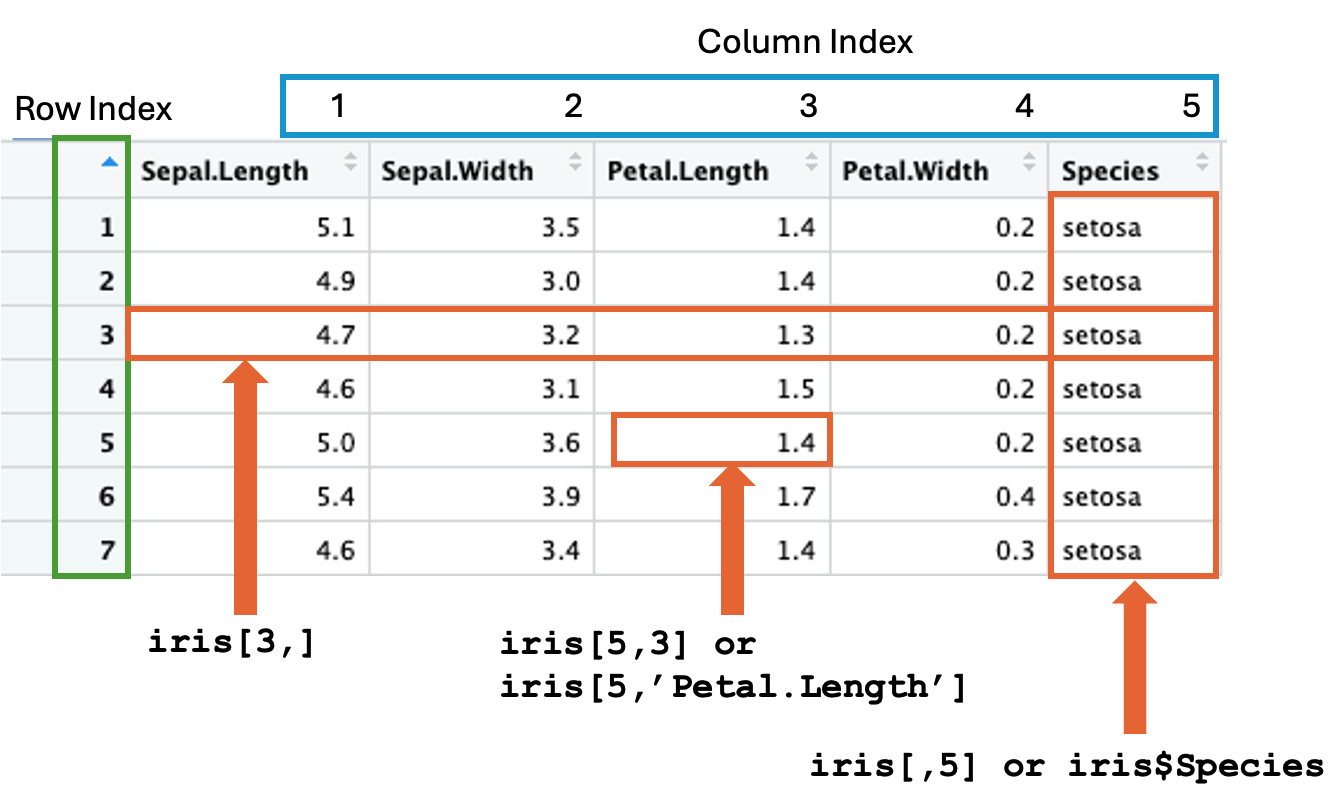
\includegraphics[keepaspectratio]{images/Figure_1.1.png}}

}

\caption{\label{fig-Fig1-1}Accessing rows and columns of a data frame.}

\end{figure}%

Similarly, if the row index is skipped, all rows of the specified
column(s) are returned. For example,

\begin{Shaded}
\begin{Highlighting}[]
\CommentTok{\# Specify only the column index.}
\FunctionTok{head}\NormalTok{(iris[,}\DecValTok{5}\NormalTok{])}
\end{Highlighting}
\end{Shaded}

\begin{verbatim}
[1] setosa setosa setosa setosa setosa setosa
Levels: setosa versicolor virginica
\end{verbatim}

Note that the \texttt{head()} above is used to limit the number of rows
displayed by avoiding listing page after page of data rows.

You are not limited to display one row or one column using this indexing
scheme. For example, show to 110\^{}th and 34\^{}th rows and
2\textsuperscript{nd} and 5\textsuperscript{th} columns,

\begin{Shaded}
\begin{Highlighting}[]
\NormalTok{iris[}\FunctionTok{c}\NormalTok{(}\DecValTok{110}\NormalTok{,}\DecValTok{34}\NormalTok{), }\FunctionTok{c}\NormalTok{(}\DecValTok{2}\NormalTok{,}\DecValTok{5}\NormalTok{)]}
\end{Highlighting}
\end{Shaded}

\begin{verbatim}
    Sepal.Width   Species
110         3.6 virginica
34          4.2    setosa
\end{verbatim}

As columns are often named \footnote{If rows are named, rows can be
  referenced by their names.}, columns can be referenced by their names
as well (Figure~\ref{fig-Fig1-1}). E.g., the \texttt{Petal.Length} of
the 5\textsuperscript{th} row:

\begin{Shaded}
\begin{Highlighting}[]
\NormalTok{iris[}\DecValTok{5}\NormalTok{,}\StringTok{\textquotesingle{}Petal.Length\textquotesingle{}}\NormalTok{]}
\end{Highlighting}
\end{Shaded}

\begin{verbatim}
[1] 1.4
\end{verbatim}

To access more than one column and row, pack the row indexes and column
names in vectors using the \texttt{c(...)} function, which
\textbf{c}ombines or \textbf{c}ollates several items into a vector
object (see Section~\ref{sec-vectors}). For example, show the
\texttt{Petal.Length} and \texttt{Sepal.Length} of the
123\textsuperscript{th} and 96\textsuperscript{th} rows:

\begin{Shaded}
\begin{Highlighting}[]
\NormalTok{iris[}\FunctionTok{c}\NormalTok{(}\DecValTok{123}\NormalTok{,}\DecValTok{96}\NormalTok{),}\FunctionTok{c}\NormalTok{(}\StringTok{\textquotesingle{}Petal.Length\textquotesingle{}}\NormalTok{,}\StringTok{\textquotesingle{}Sepal.Length\textquotesingle{}}\NormalTok{)]}
\end{Highlighting}
\end{Shaded}

\begin{verbatim}
    Petal.Length Sepal.Length
123          6.7          7.7
96           4.2          5.7
\end{verbatim}

If your task is to extract a single column, R provides an alternative
way to access a column by its name. The syntax is
\texttt{\textless{}data\ frame\ name\textgreater{}\$\textless{}column\ name\textgreater{}}
\footnote{The \texttt{\$} method only works for a single column.}. For
example, \texttt{iris\$Species}, which is equivalent to
\texttt{iris{[},5{]}},

\begin{Shaded}
\begin{Highlighting}[]
\FunctionTok{head}\NormalTok{(iris}\SpecialCharTok{$}\NormalTok{Species)}
\end{Highlighting}
\end{Shaded}

\begin{verbatim}
[1] setosa setosa setosa setosa setosa setosa
Levels: setosa versicolor virginica
\end{verbatim}

We have covered several ways to access rows, columns, or both using
indexes and column names. There are additional methods to select rows
and columns by conditions. More of this topic will be discussed in
Chapter~\ref{sec-02-data-wrangling}.

\subsubsection{Create a Data Frame}\label{create-a-data-frame}

We can use the \texttt{data.frame()} function with the concept of
vectors to create a dataset in data frame format. For example, a study
collected 10 fish with their sex and age. To create the data frame,
vectors must be created to represent each variable (column). Here's the
R code:

\begin{Shaded}
\begin{Highlighting}[]
\NormalTok{sex }\OtherTok{\textless{}{-}} \FunctionTok{c}\NormalTok{(}\StringTok{\textquotesingle{}F\textquotesingle{}}\NormalTok{,}\StringTok{\textquotesingle{}M\textquotesingle{}}\NormalTok{,}\StringTok{\textquotesingle{}M\textquotesingle{}}\NormalTok{,}\StringTok{\textquotesingle{}F\textquotesingle{}}\NormalTok{,}\StringTok{\textquotesingle{}F\textquotesingle{}}\NormalTok{,}\StringTok{\textquotesingle{}F\textquotesingle{}}\NormalTok{,}\StringTok{\textquotesingle{}M\textquotesingle{}}\NormalTok{,}\StringTok{\textquotesingle{}M\textquotesingle{}}\NormalTok{,}\StringTok{\textquotesingle{}M\textquotesingle{}}\NormalTok{,}\StringTok{\textquotesingle{}M\textquotesingle{}}\NormalTok{)}
\NormalTok{age }\OtherTok{\textless{}{-}} \FunctionTok{c}\NormalTok{(}\DecValTok{1}\NormalTok{,}\DecValTok{3}\NormalTok{,}\DecValTok{2}\NormalTok{,}\DecValTok{3}\NormalTok{,}\DecValTok{1}\NormalTok{,}\DecValTok{1}\NormalTok{,}\DecValTok{3}\NormalTok{,}\DecValTok{3}\NormalTok{,}\DecValTok{1}\NormalTok{,}\DecValTok{1}\NormalTok{)}
\NormalTok{fish }\OtherTok{\textless{}{-}} \FunctionTok{data.frame}\NormalTok{(sex,age)}
\NormalTok{fish}
\end{Highlighting}
\end{Shaded}

\begin{verbatim}
   sex age
1    F   1
2    M   3
3    M   2
4    F   3
5    F   1
6    F   1
7    M   3
8    M   3
9    M   1
10   M   1
\end{verbatim}

You can use the \texttt{summary()} function to examine the summary
statistics of the variables.

\begin{Shaded}
\begin{Highlighting}[]
\FunctionTok{summary}\NormalTok{(fish)}
\end{Highlighting}
\end{Shaded}

\begin{verbatim}
        sex          age     
 Length   :10   Min.   :1.0  
 N.unique : 2   1st Qu.:1.0  
 N.blank  : 0   Median :1.5  
 Min.nchar: 1   Mean   :1.9  
 Max.nchar: 1   3rd Qu.:3.0  
                Max.   :3.0  
\end{verbatim}

Find out more information about the \texttt{summary()} function below
Section~\ref{sec-summary-function}.

It is almost done. There is one nuance. In the current form,
\texttt{sex} is a character variable, so its summary statistics are a
bit strange. Most often, variables like that should be
categorical/nominal. Therefore, we need to convert \texttt{sex} into a
\texttt{factor} Section~\ref{sec-factor-levels}. Here's the revised
code:

\begin{Shaded}
\begin{Highlighting}[]
\NormalTok{sex }\OtherTok{\textless{}{-}} \FunctionTok{c}\NormalTok{(}\StringTok{\textquotesingle{}F\textquotesingle{}}\NormalTok{,}\StringTok{\textquotesingle{}M\textquotesingle{}}\NormalTok{,}\StringTok{\textquotesingle{}M\textquotesingle{}}\NormalTok{,}\StringTok{\textquotesingle{}F\textquotesingle{}}\NormalTok{,}\StringTok{\textquotesingle{}F\textquotesingle{}}\NormalTok{,}\StringTok{\textquotesingle{}F\textquotesingle{}}\NormalTok{,}\StringTok{\textquotesingle{}M\textquotesingle{}}\NormalTok{,}\StringTok{\textquotesingle{}M\textquotesingle{}}\NormalTok{,}\StringTok{\textquotesingle{}M\textquotesingle{}}\NormalTok{,}\StringTok{\textquotesingle{}M\textquotesingle{}}\NormalTok{)}
\NormalTok{sex }\OtherTok{\textless{}{-}} \FunctionTok{factor}\NormalTok{(sex, }\AttributeTok{levels=}\FunctionTok{c}\NormalTok{(}\StringTok{\textquotesingle{}F\textquotesingle{}}\NormalTok{,}\StringTok{\textquotesingle{}M\textquotesingle{}}\NormalTok{))}
\NormalTok{age }\OtherTok{\textless{}{-}} \FunctionTok{c}\NormalTok{(}\DecValTok{1}\NormalTok{,}\DecValTok{3}\NormalTok{,}\DecValTok{2}\NormalTok{,}\DecValTok{3}\NormalTok{,}\DecValTok{1}\NormalTok{,}\DecValTok{1}\NormalTok{,}\DecValTok{3}\NormalTok{,}\DecValTok{3}\NormalTok{,}\DecValTok{1}\NormalTok{,}\DecValTok{1}\NormalTok{)}
\NormalTok{fish }\OtherTok{\textless{}{-}} \FunctionTok{data.frame}\NormalTok{(sex,age)}
\NormalTok{fish}
\end{Highlighting}
\end{Shaded}

\begin{verbatim}
   sex age
1    F   1
2    M   3
3    M   2
4    F   3
5    F   1
6    F   1
7    M   3
8    M   3
9    M   1
10   M   1
\end{verbatim}

See the differences for \texttt{sex} after revision.

\begin{Shaded}
\begin{Highlighting}[]
\FunctionTok{summary}\NormalTok{(fish)}
\end{Highlighting}
\end{Shaded}

\begin{verbatim}
 sex        age     
 F:4   Min.   :1.0  
 M:6   1st Qu.:1.0  
       Median :1.5  
       Mean   :1.9  
       3rd Qu.:3.0  
       Max.   :3.0  
\end{verbatim}

\section{Descriptive Statistics}\label{descriptive-statistics}

\subsection{Non-robust Statistics}\label{non-robust-statistics}

Sample mean, variance, and standard deviation are non-robust statistics,
as they are sensitive to outliers (extreme values).

\begin{Shaded}
\begin{Highlighting}[]
\CommentTok{\# A sample of pumpkins\textquotesingle{} weights}
\NormalTok{pumpkins }\OtherTok{\textless{}{-}} \FunctionTok{c}\NormalTok{(}\FloatTok{6.85}\NormalTok{,}\FloatTok{6.56}\NormalTok{,}\FloatTok{6.23}\NormalTok{,}\FloatTok{7.55}\NormalTok{,}\FloatTok{4.45}\NormalTok{,}\FloatTok{10.14}\NormalTok{,}\FloatTok{3.52}\NormalTok{,}\FloatTok{6.62}\NormalTok{,}\FloatTok{3.76}\NormalTok{,}\FloatTok{7.62}\NormalTok{)}
\end{Highlighting}
\end{Shaded}

\emph{Sample Mean}

\begin{Shaded}
\begin{Highlighting}[]
\CommentTok{\# Sample mean or the average weight}
\FunctionTok{mean}\NormalTok{(pumpkins)}
\end{Highlighting}
\end{Shaded}

\begin{verbatim}
[1] 6.33
\end{verbatim}

\emph{Sample Variance}

\begin{Shaded}
\begin{Highlighting}[]
\CommentTok{\# Sample variance}
\FunctionTok{var}\NormalTok{(pumpkins)}
\end{Highlighting}
\end{Shaded}

\begin{verbatim}
[1] 4.013489
\end{verbatim}

\emph{Sample Standard Deviation}

\begin{Shaded}
\begin{Highlighting}[]
\CommentTok{\# Sample standard deviation}
\FunctionTok{sd}\NormalTok{(pumpkins)}
\end{Highlighting}
\end{Shaded}

\begin{verbatim}
[1] 2.003369
\end{verbatim}

By the way, the square root of the sample variance \(\sqrt{variance}\)
is the standard deviation. See below:

\begin{Shaded}
\begin{Highlighting}[]
\FunctionTok{sqrt}\NormalTok{(}\FunctionTok{var}\NormalTok{(pumpkins))}
\end{Highlighting}
\end{Shaded}

\begin{verbatim}
[1] 2.003369
\end{verbatim}

\subsection{Robust Statistics}\label{robust-statistics}

Median and quantiles are called robust statistics, as they reduce the
influence of outliers.

\emph{Median}

\begin{Shaded}
\begin{Highlighting}[]
\CommentTok{\# A sample of pumpkins\textquotesingle{} weights}
\NormalTok{pumpkins }\OtherTok{\textless{}{-}} \FunctionTok{c}\NormalTok{(}\FloatTok{6.85}\NormalTok{,}\FloatTok{6.56}\NormalTok{,}\FloatTok{6.23}\NormalTok{,}\FloatTok{7.55}\NormalTok{,}\FloatTok{4.45}\NormalTok{,}\FloatTok{10.14}\NormalTok{,}\FloatTok{3.52}\NormalTok{,}\FloatTok{6.62}\NormalTok{,}\FloatTok{3.76}\NormalTok{,}\FloatTok{7.62}\NormalTok{)}
\end{Highlighting}
\end{Shaded}

\begin{Shaded}
\begin{Highlighting}[]
\FunctionTok{median}\NormalTok{(pumpkins)}
\end{Highlighting}
\end{Shaded}

\begin{verbatim}
[1] 6.59
\end{verbatim}

\emph{Quantile}

The default quantile interval, as the name suggests, is 25\%. Note that
the R function name is \texttt{quantile()}, not
\st{\mbox{\texttt{quartile()}}}, as users can override the default 25\%
interval.

\begin{Shaded}
\begin{Highlighting}[]
\FunctionTok{quantile}\NormalTok{(pumpkins)}
\end{Highlighting}
\end{Shaded}

\begin{verbatim}
    0%    25%    50%    75%   100% 
 3.520  4.895  6.590  7.375 10.140 
\end{verbatim}

Instead of the default 25\% interval, you can specify your preferred
quantile(s), and they don't have to be equally divided. Here are some
examples:

\begin{Shaded}
\begin{Highlighting}[]
\FunctionTok{quantile}\NormalTok{(pumpkins, }\AttributeTok{probs =} \FunctionTok{c}\NormalTok{(}\FloatTok{0.1}\NormalTok{,}\FloatTok{0.9}\NormalTok{))}
\end{Highlighting}
\end{Shaded}

\begin{verbatim}
  10%   90% 
3.736 7.872 
\end{verbatim}

Or, a specific quantile.

\begin{Shaded}
\begin{Highlighting}[]
\FunctionTok{quantile}\NormalTok{(pumpkins, }\AttributeTok{probs =} \FunctionTok{c}\NormalTok{(}\FloatTok{0.05}\NormalTok{))}
\end{Highlighting}
\end{Shaded}

\begin{verbatim}
   5% 
3.628 
\end{verbatim}

\begin{Shaded}
\begin{Highlighting}[]
\FunctionTok{quantile}\NormalTok{(pumpkins, }\AttributeTok{probs =} \FunctionTok{c}\NormalTok{(}\FloatTok{0.95}\NormalTok{))}
\end{Highlighting}
\end{Shaded}

\begin{verbatim}
  95% 
9.006 
\end{verbatim}

\textbf{Inter-Quartile Region (IQR)}

Here is the definition of IQR:

\[IQR = Q3 - Q1\]

\begin{Shaded}
\begin{Highlighting}[]
\FunctionTok{IQR}\NormalTok{(pumpkins)}
\end{Highlighting}
\end{Shaded}

\begin{verbatim}
[1] 2.48
\end{verbatim}

IQR is used to determine the upper and lower whiskers in a boxplot. Data
points below or above the lower or upper whisker are considered
outliers.

\[Lower\space whisker = Q1 - 1.5\times{IQR}\]
\[Upper\space whisker = Q3 + 1.5\times{IQR}\]

\subsection{\texorpdfstring{\texttt{summary()}
Function}{summary() Function}}\label{sec-summary-function}

A data frame may consist of many variables of different types in various
ranges. Therefore, it makes a lot of sense to take a glimpse of all
variables before analysis. It can be done by using the
\texttt{summary()} function to reveal:

\begin{enumerate}
\def\labelenumi{\arabic{enumi}.}
\item
  The variable type of each column.
\item
  If the column is numeric, a summary of numeric values.
\item
  If the column is categorical (factor), what are the levels and order,
  if it is ordinal.
\end{enumerate}

Let's see the summary of \texttt{iris}:

\begin{Shaded}
\begin{Highlighting}[]
\FunctionTok{summary}\NormalTok{(iris)}
\end{Highlighting}
\end{Shaded}

\begin{verbatim}
  Sepal.Length    Sepal.Width     Petal.Length    Petal.Width   
 Min.   :4.300   Min.   :2.000   Min.   :1.000   Min.   :0.100  
 1st Qu.:5.100   1st Qu.:2.800   1st Qu.:1.600   1st Qu.:0.300  
 Median :5.800   Median :3.000   Median :4.350   Median :1.300  
 Mean   :5.843   Mean   :3.057   Mean   :3.758   Mean   :1.199  
 3rd Qu.:6.400   3rd Qu.:3.300   3rd Qu.:5.100   3rd Qu.:1.800  
 Max.   :7.900   Max.   :4.400   Max.   :6.900   Max.   :2.500  
       Species  
 setosa    :50  
 versicolor:50  
 virginica :50  
                
                
                
\end{verbatim}

The summary will show the range (min. and max.) and quantiles of a
numeric column. For a categorical variable (factor), it will show the
levels with the number of samples (rows) found for each level, e.g.,
\texttt{Species} is a nominal variable, with 50 samples per species.

\section{Utility Functions}\label{utility-functions}

\subsection{Inspection Functions}\label{inspection-functions}

Before diving into data analysis, we often want to know some basic
information about it, such as the number of samples, what is the range
of a numeric variable, etc. Here we discuss a few R functions to do
that, and we call them inspection functions.

We will use a sample of pumpkin weights for illustration.

\begin{Shaded}
\begin{Highlighting}[]
\CommentTok{\# A sample of pumpkins\textquotesingle{} weights}
\NormalTok{pumpkins }\OtherTok{\textless{}{-}} \FunctionTok{c}\NormalTok{(}\FloatTok{6.85}\NormalTok{,}\FloatTok{6.56}\NormalTok{,}\FloatTok{6.23}\NormalTok{,}\FloatTok{7.55}\NormalTok{,}\FloatTok{4.45}\NormalTok{,}\FloatTok{10.14}\NormalTok{,}\FloatTok{3.52}\NormalTok{,}\FloatTok{6.62}\NormalTok{,}\FloatTok{3.76}\NormalTok{,}\FloatTok{7.62}\NormalTok{)}
\end{Highlighting}
\end{Shaded}

The \texttt{length()} shows the number of items in a vector.

\begin{Shaded}
\begin{Highlighting}[]
\FunctionTok{length}\NormalTok{(pumpkins)}
\end{Highlighting}
\end{Shaded}

\begin{verbatim}
[1] 10
\end{verbatim}

To be clear, \texttt{length()} counts the number of items in an R
composite object; the number of items in a vector or the number of
columns in a data frame. \textbf{If the object is atomic, the function
will return 1.} For example, in the following example, \texttt{dna} is
an atomic, character variable. The function will return 1, not the
number of characters.

\begin{Shaded}
\begin{Highlighting}[]
\NormalTok{dna }\OtherTok{\textless{}{-}} \StringTok{\textquotesingle{}ACGTAGC\textquotesingle{}}
\FunctionTok{length}\NormalTok{(dna)}
\end{Highlighting}
\end{Shaded}

\begin{verbatim}
[1] 1
\end{verbatim}

To count the number of characters in a character variable, use the
\texttt{nchar()} function.

\begin{Shaded}
\begin{Highlighting}[]
\FunctionTok{nchar}\NormalTok{(dna)}
\end{Highlighting}
\end{Shaded}

\begin{verbatim}
[1] 7
\end{verbatim}

The \texttt{range()} prints the minimum and maximum values of an
object\footnote{Note that \texttt{range()} works for a non-numeric
  vector, but we will skip such a special operation.}.

\begin{Shaded}
\begin{Highlighting}[]
\FunctionTok{range}\NormalTok{(pumpkins)}
\end{Highlighting}
\end{Shaded}

\begin{verbatim}
[1]  3.52 10.14
\end{verbatim}

If you are interested in either the minimum or maximum, here are the
corresponding functions:

\begin{Shaded}
\begin{Highlighting}[]
\CommentTok{\# The lightest}
\FunctionTok{min}\NormalTok{(pumpkins)}
\end{Highlighting}
\end{Shaded}

\begin{verbatim}
[1] 3.52
\end{verbatim}

\begin{Shaded}
\begin{Highlighting}[]
\CommentTok{\# The heaviest}
\FunctionTok{max}\NormalTok{(pumpkins)}
\end{Highlighting}
\end{Shaded}

\begin{verbatim}
[1] 10.14
\end{verbatim}

\subsection{Printing and Formatting}\label{printing-and-formatting}

R provides a function called \texttt{print()} that prints text to the
console. E.g.,

\begin{Shaded}
\begin{Highlighting}[]
\FunctionTok{print}\NormalTok{(}\StringTok{"Hello World!"}\NormalTok{)}
\end{Highlighting}
\end{Shaded}

\begin{verbatim}
[1] "Hello World!"
\end{verbatim}

\begin{Shaded}
\begin{Highlighting}[]
\NormalTok{radius }\OtherTok{\textless{}{-}} \FloatTok{2.5}
\NormalTok{diameter }\OtherTok{\textless{}{-}} \DecValTok{2}\SpecialCharTok{*}\NormalTok{pi}\SpecialCharTok{*}\NormalTok{radius}
\FunctionTok{print}\NormalTok{(diameter)}
\end{Highlighting}
\end{Shaded}

\begin{verbatim}
[1] 15.708
\end{verbatim}

Suppose you want to improve the printout by making it more readable, say
\texttt{"The\ diameter\ of\ a\ circle\ with\ radius\ 2.5\ cm\ is\ 15.70796."}
In such a case, you need the format function \texttt{paste()}. Here's
how to use it:

\begin{Shaded}
\begin{Highlighting}[]
\NormalTok{radius }\OtherTok{\textless{}{-}} \FloatTok{2.5}
\NormalTok{diameter }\OtherTok{\textless{}{-}} \DecValTok{2}\SpecialCharTok{*}\NormalTok{pi}\SpecialCharTok{*}\NormalTok{radius}
\FunctionTok{print}\NormalTok{(}\FunctionTok{paste}\NormalTok{(}\StringTok{"The diameter of a circle with radius"}\NormalTok{,radius,}\StringTok{"cm is"}\NormalTok{,diameter,}\StringTok{"."}\NormalTok{))}
\end{Highlighting}
\end{Shaded}

\begin{verbatim}
[1] "The diameter of a circle with radius 2.5 cm is 15.708 ."
\end{verbatim}

The above printout is almost perfect. If you're picky and don't like the
extra space separating the diameter and the period in the above message,
you can use \texttt{paste()}'s cousin function \texttt{paste0()}. The
difference between the two is that \texttt{paste0()} will not
automatically add an extra space between each component given to the
function. Below is the previous print statement with \texttt{paste0()}:

\begin{Shaded}
\begin{Highlighting}[]
\FunctionTok{print}\NormalTok{(}\FunctionTok{paste0}\NormalTok{(}\StringTok{"The diameter of a circle with radius"}\NormalTok{,radius,}\StringTok{"cm is"}\NormalTok{,diameter,}\StringTok{"."}\NormalTok{))}
\end{Highlighting}
\end{Shaded}

\begin{verbatim}
[1] "The diameter of a circle with radius2.5cm is15.708."
\end{verbatim}

As you can see, there is no more space between the diameter and the
period. But it created other issues; there is no space between ``The
diameter of a circle with radius'' and the actual radius as well. So,
when you use \texttt{paste0()}, you have to take care of the space
separation yourselves. Here is the final version for using
\texttt{paste0()}:

\begin{Shaded}
\begin{Highlighting}[]
\FunctionTok{print}\NormalTok{(}\FunctionTok{paste0}\NormalTok{(}\StringTok{"The diameter of a circle with radius "}\NormalTok{,radius,}\StringTok{" cm is "}\NormalTok{,diameter,}\StringTok{"."}\NormalTok{))}
\end{Highlighting}
\end{Shaded}

\begin{verbatim}
[1] "The diameter of a circle with radius 2.5 cm is 15.708."
\end{verbatim}

\subsection{\texorpdfstring{\texttt{seq()} - create a series of
numbers}{seq() - create a series of numbers}}\label{sec-seq-function}

There are situations where we need a series of equal-interval numbers.
For example, override the default breaks - x-ticks - of a histogram, a
vector containing all possible outcomes of tossing two dice, i.e, from 2
to 12.

In R, the \texttt{seq()} function generates a list of equal-interval
numbers, whole and decimal. \texttt{seq()} takes the following
parameters:

\begin{enumerate}
\def\labelenumi{\arabic{enumi}.}
\item
  \texttt{from\ =\ 1}, the default is 1.
\item
  \texttt{to\ =\ 1}, the default is 1.
\item
  \texttt{by\ =\ 1}, the size of the interval between two adjacent
  numbers. It takes integer and decimal numbers. If it is negative, the
  series is decreasing.
\item
  \texttt{length.out} specifies how many numbers are returned. This
  option is an alternative to \texttt{by} when you care only about how
  many numbers are generated instead of the interval between them. See
  the example below.
\item
  \texttt{along.with}, it generates the same number of numbers according
  to what is provided to the \texttt{along.with} parameter.
\end{enumerate}

\textbf{Examples}

By default, \texttt{seq()} begins with 1 and has an interval of 1. E.g.,
generate 10 integers starting with 1.

\begin{Shaded}
\begin{Highlighting}[]
\FunctionTok{seq}\NormalTok{(}\DecValTok{10}\NormalTok{)}
\end{Highlighting}
\end{Shaded}

\begin{verbatim}
 [1]  1  2  3  4  5  6  7  8  9 10
\end{verbatim}

Starting from and ending with.

\begin{Shaded}
\begin{Highlighting}[]
\FunctionTok{seq}\NormalTok{(}\SpecialCharTok{{-}}\DecValTok{10}\NormalTok{,}\DecValTok{10}\NormalTok{)}
\end{Highlighting}
\end{Shaded}

\begin{verbatim}
 [1] -10  -9  -8  -7  -6  -5  -4  -3  -2  -1   0   1   2   3   4   5   6   7   8
[20]   9  10
\end{verbatim}

Specify the interval.

\begin{Shaded}
\begin{Highlighting}[]
\FunctionTok{seq}\NormalTok{(}\SpecialCharTok{{-}}\DecValTok{10}\NormalTok{,}\DecValTok{10}\NormalTok{, }\AttributeTok{by=}\DecValTok{2}\NormalTok{)}
\end{Highlighting}
\end{Shaded}

\begin{verbatim}
 [1] -10  -8  -6  -4  -2   0   2   4   6   8  10
\end{verbatim}

A decreasing sequence.

\begin{Shaded}
\begin{Highlighting}[]
\FunctionTok{seq}\NormalTok{(}\DecValTok{10}\NormalTok{,}\AttributeTok{by=}\SpecialCharTok{{-}}\DecValTok{1}\NormalTok{)}
\end{Highlighting}
\end{Shaded}

\begin{verbatim}
 [1] 10  9  8  7  6  5  4  3  2  1
\end{verbatim}

Just specify the desired numbers to be generated. As you can see, the
interval is pretty precise.

\begin{Shaded}
\begin{Highlighting}[]
\FunctionTok{seq}\NormalTok{(}\SpecialCharTok{{-}}\DecValTok{5}\NormalTok{,}\DecValTok{7}\NormalTok{,}\AttributeTok{length.out=}\DecValTok{20}\NormalTok{)}
\end{Highlighting}
\end{Shaded}

\begin{verbatim}
 [1] -5.00000000 -4.36842105 -3.73684211 -3.10526316 -2.47368421 -1.84210526
 [7] -1.21052632 -0.57894737  0.05263158  0.68421053  1.31578947  1.94736842
[13]  2.57894737  3.21052632  3.84210526  4.47368421  5.10526316  5.73684211
[19]  6.36842105  7.00000000
\end{verbatim}

Generate a sequence that matches the same number in another sequence.

\begin{Shaded}
\begin{Highlighting}[]
\NormalTok{x }\OtherTok{\textless{}{-}} \FunctionTok{seq}\NormalTok{(}\DecValTok{1}\NormalTok{,}\DecValTok{5}\NormalTok{)}
\FunctionTok{cat}\NormalTok{(}\StringTok{"x ="}\NormalTok{,x,}\StringTok{"}\SpecialCharTok{\textbackslash{}n}\StringTok{"}\NormalTok{)}
\end{Highlighting}
\end{Shaded}

\begin{verbatim}
x = 1 2 3 4 5 
\end{verbatim}

\begin{Shaded}
\begin{Highlighting}[]
\NormalTok{y }\OtherTok{\textless{}{-}} \FunctionTok{seq}\NormalTok{(}\SpecialCharTok{{-}}\DecValTok{5}\NormalTok{, }\AttributeTok{along.with=}\NormalTok{x)}
\FunctionTok{cat}\NormalTok{(}\StringTok{"y ="}\NormalTok{,y,}\StringTok{"}\SpecialCharTok{\textbackslash{}n}\StringTok{"}\NormalTok{)}
\end{Highlighting}
\end{Shaded}

\begin{verbatim}
y = -5 -4 -3 -2 -1 
\end{verbatim}

\textbf{Note:} What is the difference between \texttt{cat(...)} and
\texttt{print(paste(...))} you saw above? The main difference is that
\texttt{print(paste(...))} creates an R object (a text) and then prints
it, while \texttt{cat(...)} directly writes text to the console without
creating a formal R object. See the example below, you will understand
the nuance.

\begin{Shaded}
\begin{Highlighting}[]
\NormalTok{msg1 }\OtherTok{\textless{}{-}} \FunctionTok{print}\NormalTok{(}\FunctionTok{paste}\NormalTok{(}\StringTok{"Hello"}\NormalTok{,}\StringTok{"World"}\NormalTok{))}
\end{Highlighting}
\end{Shaded}

\begin{verbatim}
[1] "Hello World"
\end{verbatim}

\begin{Shaded}
\begin{Highlighting}[]
\FunctionTok{print}\NormalTok{(msg1)}
\end{Highlighting}
\end{Shaded}

\begin{verbatim}
[1] "Hello World"
\end{verbatim}

\begin{Shaded}
\begin{Highlighting}[]
\NormalTok{msg2 }\OtherTok{\textless{}{-}} \FunctionTok{cat}\NormalTok{(}\StringTok{"Hello"}\NormalTok{,}\StringTok{"World"}\NormalTok{,}\StringTok{"}\SpecialCharTok{\textbackslash{}n}\StringTok{"}\NormalTok{)}
\end{Highlighting}
\end{Shaded}

\begin{verbatim}
Hello World 
\end{verbatim}

\begin{Shaded}
\begin{Highlighting}[]
\FunctionTok{print}\NormalTok{(msg2)}
\end{Highlighting}
\end{Shaded}

\begin{verbatim}
NULL
\end{verbatim}

Is it really important? No, unless you're an R developer.

\subsection{\texorpdfstring{\texttt{with()}}{with()}}\label{with}

The function sets up the context of a data frame so it spares you from
using the \texttt{\$} to access the columns of a data frame, as it often
leads to longer commands, which makes it harder to comprehend and
troubleshoot. It is also commonly used together with a function applied
to one or more columns. E.g., the median of \texttt{Petal.Width}. It can
be done in two ways:

\begin{Shaded}
\begin{Highlighting}[]
\CommentTok{\# Use $}
\FunctionTok{median}\NormalTok{(iris}\SpecialCharTok{$}\NormalTok{Petal.Width)}
\end{Highlighting}
\end{Shaded}

\begin{verbatim}
[1] 1.3
\end{verbatim}

\begin{Shaded}
\begin{Highlighting}[]
\CommentTok{\# Or, use with()}
\FunctionTok{with}\NormalTok{(iris, }\FunctionTok{median}\NormalTok{(Petal.Width))}
\end{Highlighting}
\end{Shaded}

\begin{verbatim}
[1] 1.3
\end{verbatim}

For the straightforward example above, you do not see the value of
\texttt{with()}. Let's consider a more complicated row selection
example. Find \texttt{Sepal.Length} in \texttt{iris} where its
\texttt{Petal.Length} is less than 4 and \texttt{Petal.Width} is greater
than 1. The \texttt{\$}-way is:

\begin{Shaded}
\begin{Highlighting}[]
\NormalTok{iris}\SpecialCharTok{$}\NormalTok{Sepal.Length[iris}\SpecialCharTok{$}\NormalTok{Petal.Length}\SpecialCharTok{\textless{}}\DecValTok{4} \SpecialCharTok{\&}\NormalTok{ iris}\SpecialCharTok{$}\NormalTok{Petal.Width}\SpecialCharTok{\textgreater{}}\DecValTok{1}\NormalTok{]}
\end{Highlighting}
\end{Shaded}

\begin{verbatim}
[1] 5.2 5.6 5.6 5.5 5.8 5.1
\end{verbatim}

Here's the \texttt{with()} version that saves typing \texttt{iris}
repeatedly.

\begin{Shaded}
\begin{Highlighting}[]
\FunctionTok{with}\NormalTok{(iris, Sepal.Length[Petal.Length}\SpecialCharTok{\textless{}}\DecValTok{4} \SpecialCharTok{\&}\NormalTok{ Petal.Width}\SpecialCharTok{\textgreater{}}\DecValTok{1}\NormalTok{])}
\end{Highlighting}
\end{Shaded}

\begin{verbatim}
[1] 5.2 5.6 5.6 5.5 5.8 5.1
\end{verbatim}

In short, \texttt{with()} is English, so it improves the readability of
R statements. Second, it saves some typing of the data frame's name. I
recommend using \texttt{with()} whenever possible.

\section{Summary}\label{summary}

That's the bare minimum of R scripting required for data analysis. In
the next chapter, we will focus on operations applied to data frames.
Before you leave, it is useful to recap the R functions discussed in
this chapter:

\begin{longtable}[]{@{}llll@{}}
\caption{A Summary of R Operators and Functions}\tabularnewline
\toprule\noalign{}
\endfirsthead
\endhead
\bottomrule\noalign{}
\endlastfoot
\texttt{\textless{}-} & \texttt{head()} & \texttt{sd()} & + \\
\texttt{c()} & \texttt{tail()} & \texttt{range()} & - \\
\texttt{print()} & \texttt{dim()} & \texttt{min()} & * \\
\texttt{paste()} & \texttt{nrow()} & \texttt{max()} & / \\
\texttt{paste0()} & \texttt{ncol()} & \texttt{median()} & ** \\
\texttt{cat()} & \texttt{data.frame()} & \texttt{quantile()} & \^{} \\
\texttt{typeof()} & \texttt{summary()} & \texttt{IQR()} & == \\
\texttt{nchar()} & \texttt{mean()} & \texttt{seq()} &
\texttt{\textless{}-} \\
\texttt{factor()} & \texttt{var()} & \texttt{with()} & \texttt{c()} \\
\end{longtable}

\chapter{Data Wrangling}\label{sec-02-data-wrangling}

Data wrangling refers to the way to view, change, and reorganize rows
and columns in a data frame. Before we dive into the operations, it is
important to know that there are two distinct schools of data wrangling:
base R and \texttt{tidyverse}. The base R approach means that no
additional packages are required, but the \texttt{tidyverse} approach
requires the installation of \texttt{tidyverse}, even though the
installation is very straightforward. In my opinion, \texttt{tidyverse}
has substantially refined and enhanced data wrangling. You will see it
in this chapter. Regardless, we will discuss both approaches. Let's
start with the base R version.

\section*{Learning Objectives:}\label{learning-objectives-1}
\addcontentsline{toc}{section}{Learning Objectives:}

\markright{Learning Objectives:}

This chapter covers common data wrangling techniques. After finishing
this chapter, you should be able to:

\begin{itemize}
\item
  Select rows that fulfill specified conditions.
\item
  Randomly sample rows from a data frame.
\item
  Sort rows in a data frame.
\item
  Select a subset of columns.
\item
  Add and remove columns to an existing data frame.
\item
  Tabulate data.
\end{itemize}

\section{Base R}\label{base-r}

\subsection{Select Rows by
Condition(s)}\label{select-rows-by-conditions}

The \texttt{subset()} function selects rows if they satisfy the
condition(s). Below are six relational operators:

\begin{enumerate}
\def\labelenumi{\arabic{enumi}.}
\item
  \texttt{\textgreater{}} greater than.
\item
  \texttt{\textgreater{}=}\footnote{No spaces between the two symbols.}
  greater than or equal to.
\item
  \texttt{\textless{}} less than.
\item
  \texttt{\textless{}=}\footnote{No spaces between the two symbols.}
  less than or equal to.
\item
  \texttt{==}\footnote{No spaces between the two symbols.} equal to.
\item
  \texttt{!=}\footnote{No spaces between the two symbols.} not equal to.
\end{enumerate}

If the selection involves multiple conditions, they must be specified in
conjunction with relational operators. Here are the three logical
operators required for multi-parts conditions:

\begin{enumerate}
\def\labelenumi{\arabic{enumi}.}
\item
  \texttt{\textbar{}} denotes the logical OR.
\item
  \texttt{\&} denotes the logical AND.
\item
  \texttt{!} denotes the logical NOT.
\end{enumerate}

\subsubsection{\texorpdfstring{\texttt{subset()} with
Vectors}{subset() with Vectors}}\label{subset-with-vectors}

Let's define a vector.

\begin{Shaded}
\begin{Highlighting}[]
\CommentTok{\# A sample of pumpkins\textquotesingle{} weights}
\NormalTok{pumpkins }\OtherTok{\textless{}{-}} \FunctionTok{c}\NormalTok{(}\FloatTok{6.85}\NormalTok{,}\FloatTok{6.56}\NormalTok{,}\FloatTok{6.23}\NormalTok{,}\FloatTok{7.55}\NormalTok{,}\FloatTok{4.45}\NormalTok{,}\FloatTok{10.14}\NormalTok{,}\FloatTok{3.52}\NormalTok{,}\FloatTok{6.62}\NormalTok{,}\FloatTok{3.76}\NormalTok{,}\FloatTok{7.62}\NormalTok{, }\DecValTok{7}\NormalTok{)}
\end{Highlighting}
\end{Shaded}

Select pumpkins heavier than 7 lbs.

\begin{Shaded}
\begin{Highlighting}[]
\FunctionTok{subset}\NormalTok{(pumpkins, pumpkins}\SpecialCharTok{\textgreater{}}\DecValTok{7}\NormalTok{)}
\end{Highlighting}
\end{Shaded}

\begin{verbatim}
[1]  7.55 10.14  7.62
\end{verbatim}

Select pumpkins is exactly 7 lbs.

\begin{Shaded}
\begin{Highlighting}[]
\FunctionTok{subset}\NormalTok{(pumpkins, pumpkins}\SpecialCharTok{==}\DecValTok{7}\NormalTok{)}
\end{Highlighting}
\end{Shaded}

\begin{verbatim}
[1] 7
\end{verbatim}

Select pumpkins between 6 and 7 lbs, inclusive.

\begin{Shaded}
\begin{Highlighting}[]
\FunctionTok{subset}\NormalTok{(pumpkins, pumpkins}\SpecialCharTok{\textgreater{}=}\DecValTok{6} \SpecialCharTok{\&}\NormalTok{ pumpkins}\SpecialCharTok{\textless{}=}\DecValTok{7}\NormalTok{)}
\end{Highlighting}
\end{Shaded}

\begin{verbatim}
[1] 6.85 6.56 6.23 6.62 7.00
\end{verbatim}

\subsubsection{\texorpdfstring{\texttt{subset()} with Data
Frames}{subset() with Data Frames}}\label{subset-with-data-frames}

Here is an example that chooses only the \texttt{setosa} species from
\texttt{iris} data frame and keeps them in a new data frame. Note that
the equality check is case-sensitive.

\begin{Shaded}
\begin{Highlighting}[]
\NormalTok{setosa\_iris }\OtherTok{\textless{}{-}} \FunctionTok{subset}\NormalTok{(iris, Species }\SpecialCharTok{==} \StringTok{\textquotesingle{}setosa\textquotesingle{}}\NormalTok{)}

\CommentTok{\# How many are selected?}
\FunctionTok{print}\NormalTok{(}\FunctionTok{paste}\NormalTok{(}\StringTok{"There are"}\NormalTok{, }\FunctionTok{nrow}\NormalTok{(setosa\_iris), }\StringTok{"rows."}\NormalTok{))}
\end{Highlighting}
\end{Shaded}

\begin{verbatim}
[1] "There are 50 rows."
\end{verbatim}

\begin{Shaded}
\begin{Highlighting}[]
\CommentTok{\# Peek into the first few rows of the result.}
\FunctionTok{head}\NormalTok{(setosa\_iris)}
\end{Highlighting}
\end{Shaded}

\begin{verbatim}
  Sepal.Length Sepal.Width Petal.Length Petal.Width Species
1          5.1         3.5          1.4         0.2  setosa
2          4.9         3.0          1.4         0.2  setosa
3          4.7         3.2          1.3         0.2  setosa
4          4.6         3.1          1.5         0.2  setosa
5          5.0         3.6          1.4         0.2  setosa
6          5.4         3.9          1.7         0.4  setosa
\end{verbatim}

More than one condition. Select rows with \texttt{Sepal.Length} is
greater than 5 or Sepal.Width` is smaller than 3.

\begin{Shaded}
\begin{Highlighting}[]
\NormalTok{iris\_or\_eg }\OtherTok{\textless{}{-}} \FunctionTok{subset}\NormalTok{(iris, Sepal.Length }\SpecialCharTok{\textgreater{}} \DecValTok{5} \SpecialCharTok{|}\NormalTok{ Sepal.Width }\SpecialCharTok{\textless{}} \DecValTok{3}\NormalTok{ )}

\CommentTok{\# How many?}
\FunctionTok{print}\NormalTok{(}\FunctionTok{paste}\NormalTok{(}\StringTok{"There are"}\NormalTok{, }\FunctionTok{nrow}\NormalTok{(iris\_or\_eg), }\StringTok{"rows."}\NormalTok{))}
\end{Highlighting}
\end{Shaded}

\begin{verbatim}
[1] "There are 124 rows."
\end{verbatim}

\begin{Shaded}
\begin{Highlighting}[]
\FunctionTok{head}\NormalTok{(iris\_or\_eg)}
\end{Highlighting}
\end{Shaded}

\begin{verbatim}
   Sepal.Length Sepal.Width Petal.Length Petal.Width Species
1           5.1         3.5          1.4         0.2  setosa
6           5.4         3.9          1.7         0.4  setosa
9           4.4         2.9          1.4         0.2  setosa
11          5.4         3.7          1.5         0.2  setosa
15          5.8         4.0          1.2         0.2  setosa
16          5.7         4.4          1.5         0.4  setosa
\end{verbatim}

Select rows with \texttt{Petal.Length} is greater than 6 and
Petal.Width` is smaller than 2.

\begin{Shaded}
\begin{Highlighting}[]
\CommentTok{\# More than one condition. The relational AND operator.}
\NormalTok{iris\_and\_eg }\OtherTok{\textless{}{-}} \FunctionTok{subset}\NormalTok{(iris, Petal.Length }\SpecialCharTok{\textgreater{}} \DecValTok{6} \SpecialCharTok{\&}\NormalTok{ Petal.Width }\SpecialCharTok{\textless{}} \DecValTok{2}\NormalTok{ )}

\CommentTok{\# How many?}
\FunctionTok{print}\NormalTok{(}\FunctionTok{paste}\NormalTok{(}\StringTok{"There are"}\NormalTok{, }\FunctionTok{nrow}\NormalTok{(iris\_and\_eg), }\StringTok{"rows."}\NormalTok{))}
\end{Highlighting}
\end{Shaded}

\begin{verbatim}
[1] "There are 2 rows."
\end{verbatim}

\begin{Shaded}
\begin{Highlighting}[]
\NormalTok{iris\_and\_eg}
\end{Highlighting}
\end{Shaded}

\begin{verbatim}
    Sepal.Length Sepal.Width Petal.Length Petal.Width   Species
108          7.3         2.9          6.3         1.8 virginica
131          7.4         2.8          6.1         1.9 virginica
\end{verbatim}

Select everything except for \texttt{setosa}.

\begin{Shaded}
\begin{Highlighting}[]
\CommentTok{\# No setosa iris}
\NormalTok{iris\_no\_setosa\_eg }\OtherTok{\textless{}{-}} \FunctionTok{subset}\NormalTok{(iris, Species }\SpecialCharTok{!=} \StringTok{\textquotesingle{}setosa\textquotesingle{}}\NormalTok{)}

\CommentTok{\# How many?}
\FunctionTok{print}\NormalTok{(}\FunctionTok{paste}\NormalTok{(}\StringTok{"There are"}\NormalTok{, }\FunctionTok{nrow}\NormalTok{(iris\_no\_setosa\_eg), }\StringTok{"rows."}\NormalTok{))}
\end{Highlighting}
\end{Shaded}

\begin{verbatim}
[1] "There are 100 rows."
\end{verbatim}

\begin{Shaded}
\begin{Highlighting}[]
\FunctionTok{head}\NormalTok{(iris\_no\_setosa\_eg)}
\end{Highlighting}
\end{Shaded}

\begin{verbatim}
   Sepal.Length Sepal.Width Petal.Length Petal.Width    Species
51          7.0         3.2          4.7         1.4 versicolor
52          6.4         3.2          4.5         1.5 versicolor
53          6.9         3.1          4.9         1.5 versicolor
54          5.5         2.3          4.0         1.3 versicolor
55          6.5         2.8          4.6         1.5 versicolor
56          5.7         2.8          4.5         1.3 versicolor
\end{verbatim}

\subsection{Random Sampling}\label{random-sampling}

It is quite common to randomly sample a subset of items from a vector or
rows from a data frame.

\subsubsection{Sample Items Randomly from a
Vector}\label{sample-items-randomly-from-a-vector}

\begin{Shaded}
\begin{Highlighting}[]
\CommentTok{\# A sample of pumpkins\textquotesingle{} weights}
\NormalTok{pumpkins }\OtherTok{\textless{}{-}} \FunctionTok{c}\NormalTok{(}\FloatTok{6.85}\NormalTok{,}\FloatTok{6.56}\NormalTok{,}\FloatTok{6.23}\NormalTok{,}\FloatTok{7.55}\NormalTok{,}\FloatTok{4.45}\NormalTok{,}\FloatTok{10.14}\NormalTok{,}\FloatTok{3.52}\NormalTok{,}\FloatTok{6.62}\NormalTok{,}\FloatTok{3.76}\NormalTok{,}\FloatTok{7.62}\NormalTok{, }\DecValTok{7}\NormalTok{)}
\end{Highlighting}
\end{Shaded}

Randomly pick 5 samples without replacement.

\begin{Shaded}
\begin{Highlighting}[]
\FunctionTok{sample}\NormalTok{(pumpkins, }\AttributeTok{size=}\DecValTok{5}\NormalTok{, }\AttributeTok{replace=}\NormalTok{F)}
\end{Highlighting}
\end{Shaded}

\begin{verbatim}
[1] 6.56 6.62 7.00 6.23 3.52
\end{verbatim}

The \texttt{replace=} option can be twisted to simulate tossing a coin N
times. E.g.,

\begin{Shaded}
\begin{Highlighting}[]
\FunctionTok{sample}\NormalTok{(}\FunctionTok{c}\NormalTok{(}\StringTok{\textquotesingle{}H\textquotesingle{}}\NormalTok{,}\StringTok{\textquotesingle{}T\textquotesingle{}}\NormalTok{), }\AttributeTok{size=}\DecValTok{10}\NormalTok{, }\AttributeTok{replace=}\NormalTok{T)}
\end{Highlighting}
\end{Shaded}

\begin{verbatim}
 [1] "T" "T" "H" "H" "H" "T" "H" "H" "T" "H"
\end{verbatim}

\subsubsection{Sample Rows Randomly from a Data
Frame}\label{sample-rows-randomly-from-a-data-frame}

Let say we want to randomly pick 5 samples from \texttt{iris}. It takes
to two steps to do that:

\textbf{Step 1:} Create a list (vector) of random row indexes by the
\texttt{sample()} function. Specify the following parameters:

a.) The range of indexes. In this example, the range is from 1 to the
last row of \texttt{iris}, which can be obtained from
\texttt{nrow(iris)}.

\begin{enumerate}
\def\labelenumi{\alph{enumi})}
\setcounter{enumi}{1}
\item
  How many samples, e.g., \texttt{size\ =\ 5}.
\item
  Can a sample be drawn repeatedly? If not, \texttt{replace\ =\ F}.
\end{enumerate}

\begin{Shaded}
\begin{Highlighting}[]
\NormalTok{rnd\_idx }\OtherTok{\textless{}{-}} \FunctionTok{sample}\NormalTok{(}\FunctionTok{seq}\NormalTok{(}\FunctionTok{nrow}\NormalTok{(iris)), }\AttributeTok{size =} \DecValTok{5}\NormalTok{, }\AttributeTok{replace =}\NormalTok{ F)}
\NormalTok{rnd\_idx}
\end{Highlighting}
\end{Shaded}

\begin{verbatim}
[1] 25 62 38 16 44
\end{verbatim}

\texttt{seq(nrow(iris))} generates a vector containing 1, 2, 3, \ldots,
150.

\textbf{Step 2:} Select rows from iris according to the indexes in
\texttt{rnd\_idx}.

\begin{Shaded}
\begin{Highlighting}[]
\NormalTok{a\_random\_sample }\OtherTok{\textless{}{-}}\NormalTok{ iris[rnd\_idx,]}

\NormalTok{a\_random\_sample}
\end{Highlighting}
\end{Shaded}

\begin{verbatim}
   Sepal.Length Sepal.Width Petal.Length Petal.Width    Species
25          4.8         3.4          1.9         0.2     setosa
62          5.9         3.0          4.2         1.5 versicolor
38          4.9         3.6          1.4         0.1     setosa
16          5.7         4.4          1.5         0.4     setosa
44          5.0         3.5          1.6         0.6     setosa
\end{verbatim}

The indexing method is based on the previous chapter. Check out here:
Section~\ref{sec-access-rows-columns}.

\subsection{Sort Items}\label{sort-items}

\subsubsection{Sort Items in a Vector}\label{sort-items-in-a-vector}

It can be done using the \texttt{sort()} function.

\begin{Shaded}
\begin{Highlighting}[]
\FunctionTok{sort}\NormalTok{(pumpkins)}
\end{Highlighting}
\end{Shaded}

\begin{verbatim}
 [1]  3.52  3.76  4.45  6.23  6.56  6.62  6.85  7.00  7.55  7.62 10.14
\end{verbatim}

Sort it descending order (large to small).

\begin{Shaded}
\begin{Highlighting}[]
\FunctionTok{sort}\NormalTok{(pumpkins, }\AttributeTok{decreasing =} \ConstantTok{TRUE}\NormalTok{)}
\end{Highlighting}
\end{Shaded}

\begin{verbatim}
 [1] 10.14  7.62  7.55  7.00  6.85  6.62  6.56  6.23  4.45  3.76  3.52
\end{verbatim}

\subsubsection{Sort Rows in a Data
Frame}\label{sort-rows-in-a-data-frame}

Unfortunately, the \texttt{sort()} function does not work for the
two-dimensional data frame. We have to use the method similar to
sampling rows. It takes two steps to sort rows in a certain order.
Suppose you want to sort rows in \texttt{iris} by \texttt{Sepal.Length}
in ascending order (small to large).

\textbf{Step 1:} Obtain a list (vector) of row indexes that reflects the
sorting order of the data frame.

\begin{Shaded}
\begin{Highlighting}[]
\NormalTok{sorted\_idx }\OtherTok{\textless{}{-}} \FunctionTok{order}\NormalTok{(iris}\SpecialCharTok{$}\NormalTok{Sepal.Length)}
\NormalTok{sorted\_idx}
\end{Highlighting}
\end{Shaded}

\begin{verbatim}
  [1]  14   9  39  43  42   4   7  23  48   3  30  12  13  25  31  46   2  10
 [19]  35  38  58 107   5   8  26  27  36  41  44  50  61  94   1  18  20  22
 [37]  24  40  45  47  99  28  29  33  60  49   6  11  17  21  32  85  34  37
 [55]  54  81  82  90  91  65  67  70  89  95 122  16  19  56  80  96  97 100
 [73] 114  15  68  83  93 102 115 143  62  71 150  63  79  84  86 120 139  64
 [91]  72  74  92 128 135  69  98 127 149  57  73  88 101 104 124 134 137 147
[109]  52  75 112 116 129 133 138  55 105 111 117 148  59  76  66  78  87 109
[127] 125 141 145 146  77 113 144  53 121 140 142  51 103 110 126 130 108 131
[145] 106 118 119 123 136 132
\end{verbatim}

\textbf{Step 2:} Rearrange the rows in the data frame according to the
sorted row indexes.

\begin{Shaded}
\begin{Highlighting}[]
\CommentTok{\# The 5 shortest Sepal Lengths}
\FunctionTok{head}\NormalTok{(iris[sorted\_idx,])}
\end{Highlighting}
\end{Shaded}

\begin{verbatim}
   Sepal.Length Sepal.Width Petal.Length Petal.Width Species
14          4.3         3.0          1.1         0.1  setosa
9           4.4         2.9          1.4         0.2  setosa
39          4.4         3.0          1.3         0.2  setosa
43          4.4         3.2          1.3         0.2  setosa
42          4.5         2.3          1.3         0.3  setosa
4           4.6         3.1          1.5         0.2  setosa
\end{verbatim}

\begin{Shaded}
\begin{Highlighting}[]
\CommentTok{\# The 5 longest Sepal Lengths}
\FunctionTok{tail}\NormalTok{(iris[sorted\_idx,])}
\end{Highlighting}
\end{Shaded}

\begin{verbatim}
    Sepal.Length Sepal.Width Petal.Length Petal.Width   Species
106          7.6         3.0          6.6         2.1 virginica
118          7.7         3.8          6.7         2.2 virginica
119          7.7         2.6          6.9         2.3 virginica
123          7.7         2.8          6.7         2.0 virginica
136          7.7         3.0          6.1         2.3 virginica
132          7.9         3.8          6.4         2.0 virginica
\end{verbatim}

Note that the steps above do NOT change the original order of the rows
in the data frame. If you intend to change the row order permanently,
use the assignment operator to update the existing data frame or create
a new data frame to store the sorted rows. See below:

\begin{Shaded}
\begin{Highlighting}[]
\NormalTok{ascending\_iris }\OtherTok{\textless{}{-}}\NormalTok{ iris[sorted\_idx,]}

\CommentTok{\# The shortest Sepal Length}
\FunctionTok{head}\NormalTok{(ascending\_iris)}
\end{Highlighting}
\end{Shaded}

\begin{verbatim}
   Sepal.Length Sepal.Width Petal.Length Petal.Width Species
14          4.3         3.0          1.1         0.1  setosa
9           4.4         2.9          1.4         0.2  setosa
39          4.4         3.0          1.3         0.2  setosa
43          4.4         3.2          1.3         0.2  setosa
42          4.5         2.3          1.3         0.3  setosa
4           4.6         3.1          1.5         0.2  setosa
\end{verbatim}

\begin{Shaded}
\begin{Highlighting}[]
\CommentTok{\# The longest Sepal Length}
\FunctionTok{tail}\NormalTok{(ascending\_iris)}
\end{Highlighting}
\end{Shaded}

\begin{verbatim}
    Sepal.Length Sepal.Width Petal.Length Petal.Width   Species
106          7.6         3.0          6.6         2.1 virginica
118          7.7         3.8          6.7         2.2 virginica
119          7.7         2.6          6.9         2.3 virginica
123          7.7         2.8          6.7         2.0 virginica
136          7.7         3.0          6.1         2.3 virginica
132          7.9         3.8          6.4         2.0 virginica
\end{verbatim}

To sort rows in descending order (large to small), add the parameter
\texttt{decreasing\ =\ T} to the \texttt{order()} function.

\begin{Shaded}
\begin{Highlighting}[]
\NormalTok{desc\_idx }\OtherTok{\textless{}{-}} \FunctionTok{order}\NormalTok{(iris}\SpecialCharTok{$}\NormalTok{Sepal.Length, }\AttributeTok{decreasing =}\NormalTok{ T)}
\NormalTok{desc\_idx}
\end{Highlighting}
\end{Shaded}

\begin{verbatim}
  [1] 132 118 119 123 136 106 131 108 110 126 130 103  51  53 121 140 142  77
 [19] 113 144  66  78  87 109 125 141 145 146  59  76  55 105 111 117 148  52
 [37]  75 112 116 129 133 138  57  73  88 101 104 124 134 137 147  69  98 127
 [55] 149  64  72  74  92 128 135  63  79  84  86 120 139  62  71 150  15  68
 [73]  83  93 102 115 143  16  19  56  80  96  97 100 114  65  67  70  89  95
 [91] 122  34  37  54  81  82  90  91   6  11  17  21  32  85  49  28  29  33
[109]  60   1  18  20  22  24  40  45  47  99   5   8  26  27  36  41  44  50
[127]  61  94   2  10  35  38  58 107  12  13  25  31  46   3  30   4   7  23
[145]  48  42   9  39  43  14
\end{verbatim}

\begin{Shaded}
\begin{Highlighting}[]
\NormalTok{decreasing\_iris }\OtherTok{\textless{}{-}}\NormalTok{ iris[desc\_idx,]}
\FunctionTok{head}\NormalTok{(decreasing\_iris)}
\end{Highlighting}
\end{Shaded}

\begin{verbatim}
    Sepal.Length Sepal.Width Petal.Length Petal.Width   Species
132          7.9         3.8          6.4         2.0 virginica
118          7.7         3.8          6.7         2.2 virginica
119          7.7         2.6          6.9         2.3 virginica
123          7.7         2.8          6.7         2.0 virginica
136          7.7         3.0          6.1         2.3 virginica
106          7.6         3.0          6.6         2.1 virginica
\end{verbatim}

\begin{Shaded}
\begin{Highlighting}[]
\FunctionTok{tail}\NormalTok{(decreasing\_iris)}
\end{Highlighting}
\end{Shaded}

\begin{verbatim}
   Sepal.Length Sepal.Width Petal.Length Petal.Width Species
48          4.6         3.2          1.4         0.2  setosa
42          4.5         2.3          1.3         0.3  setosa
9           4.4         2.9          1.4         0.2  setosa
39          4.4         3.0          1.3         0.2  setosa
43          4.4         3.2          1.3         0.2  setosa
14          4.3         3.0          1.1         0.1  setosa
\end{verbatim}

\subsection{Rearranging Columns}\label{rearranging-columns}

Suppose you want to move the \texttt{Species} column to the leftmost
position. It can be done in two ways.

\begin{Shaded}
\begin{Highlighting}[]
\CommentTok{\# Reorder columns by name}
\NormalTok{new\_iris }\OtherTok{\textless{}{-}}\NormalTok{ iris[,}\FunctionTok{c}\NormalTok{(}\StringTok{"Species"}\NormalTok{,}\StringTok{"Sepal.Length"}\NormalTok{,}\StringTok{"Sepal.Width"}\NormalTok{,}\StringTok{"Petal.Length"}\NormalTok{,}\StringTok{"Petal.Width"}\NormalTok{)]}
\FunctionTok{head}\NormalTok{(new\_iris)}
\end{Highlighting}
\end{Shaded}

\begin{verbatim}
  Species Sepal.Length Sepal.Width Petal.Length Petal.Width
1  setosa          5.1         3.5          1.4         0.2
2  setosa          4.9         3.0          1.4         0.2
3  setosa          4.7         3.2          1.3         0.2
4  setosa          4.6         3.1          1.5         0.2
5  setosa          5.0         3.6          1.4         0.2
6  setosa          5.4         3.9          1.7         0.4
\end{verbatim}

\begin{Shaded}
\begin{Highlighting}[]
\CommentTok{\# Reorder columns by index}
\NormalTok{new\_iris }\OtherTok{\textless{}{-}}\NormalTok{ iris[,}\FunctionTok{c}\NormalTok{(}\DecValTok{5}\NormalTok{,}\DecValTok{1}\NormalTok{,}\DecValTok{2}\NormalTok{,}\DecValTok{3}\NormalTok{,}\DecValTok{4}\NormalTok{)]}
\FunctionTok{head}\NormalTok{(new\_iris)}
\end{Highlighting}
\end{Shaded}

\begin{verbatim}
  Species Sepal.Length Sepal.Width Petal.Length Petal.Width
1  setosa          5.1         3.5          1.4         0.2
2  setosa          4.9         3.0          1.4         0.2
3  setosa          4.7         3.2          1.3         0.2
4  setosa          4.6         3.1          1.5         0.2
5  setosa          5.0         3.6          1.4         0.2
6  setosa          5.4         3.9          1.7         0.4
\end{verbatim}

Note that if a data frame contains many columns, say \textgreater100,
this method is daunting. A much better way can be done using
\texttt{tidyverse}, so stay tuned.

\subsection{Focus on a Subset of
Columns}\label{focus-on-a-subset-of-columns}

If a data frame contains many columns, way more than you need for
analysis. It is neat to focus on those columns and leave out the rest.
Let's suppose you want to focus only on sepal information and species.

\begin{Shaded}
\begin{Highlighting}[]
\NormalTok{sepal\_iris }\OtherTok{\textless{}{-}}\NormalTok{ iris[,}\FunctionTok{c}\NormalTok{(}\StringTok{"Sepal.Length"}\NormalTok{,}\StringTok{"Sepal.Width"}\NormalTok{,}\StringTok{"Species"}\NormalTok{)]}
\FunctionTok{dim}\NormalTok{(sepal\_iris)}
\end{Highlighting}
\end{Shaded}

\begin{verbatim}
[1] 150   3
\end{verbatim}

\begin{Shaded}
\begin{Highlighting}[]
\FunctionTok{head}\NormalTok{(sepal\_iris)}
\end{Highlighting}
\end{Shaded}

\begin{verbatim}
  Sepal.Length Sepal.Width Species
1          5.1         3.5  setosa
2          4.9         3.0  setosa
3          4.7         3.2  setosa
4          4.6         3.1  setosa
5          5.0         3.6  setosa
6          5.4         3.9  setosa
\end{verbatim}

\subsection{Add a New Column}\label{add-a-new-column}

Suppose we want to add a new column called \texttt{Sepal.Ratio}, which
is the ratio \texttt{Sepal.Length} to \texttt{Sepal.Width}. Here is the
code:

\begin{Shaded}
\begin{Highlighting}[]
\NormalTok{iris}\SpecialCharTok{$}\NormalTok{Sepal.Ratio }\OtherTok{\textless{}{-}}\NormalTok{ iris}\SpecialCharTok{$}\NormalTok{Sepal.Length}\SpecialCharTok{/}\NormalTok{iris}\SpecialCharTok{$}\NormalTok{Sepal.Width}
\FunctionTok{head}\NormalTok{(iris)}
\end{Highlighting}
\end{Shaded}

\begin{verbatim}
  Sepal.Length Sepal.Width Petal.Length Petal.Width Species Sepal.Ratio
1          5.1         3.5          1.4         0.2  setosa    1.457143
2          4.9         3.0          1.4         0.2  setosa    1.633333
3          4.7         3.2          1.3         0.2  setosa    1.468750
4          4.6         3.1          1.5         0.2  setosa    1.483871
5          5.0         3.6          1.4         0.2  setosa    1.388889
6          5.4         3.9          1.7         0.4  setosa    1.384615
\end{verbatim}

You can see the new column \texttt{Sepal.Ratio} is added to the
rightmost position.

Suppose you want to add a new column that records the name of the
researcher who collected the sample. If it is done by one researcher,
you don't have to repeat the same name in a vector. Here is the code:

\begin{Shaded}
\begin{Highlighting}[]
\NormalTok{iris}\SpecialCharTok{$}\NormalTok{Researcher }\OtherTok{\textless{}{-}} \StringTok{"Brian"}
\FunctionTok{head}\NormalTok{(iris)}
\end{Highlighting}
\end{Shaded}

\begin{verbatim}
  Sepal.Length Sepal.Width Petal.Length Petal.Width Species Sepal.Ratio
1          5.1         3.5          1.4         0.2  setosa    1.457143
2          4.9         3.0          1.4         0.2  setosa    1.633333
3          4.7         3.2          1.3         0.2  setosa    1.468750
4          4.6         3.1          1.5         0.2  setosa    1.483871
5          5.0         3.6          1.4         0.2  setosa    1.388889
6          5.4         3.9          1.7         0.4  setosa    1.384615
  Researcher
1      Brian
2      Brian
3      Brian
4      Brian
5      Brian
6      Brian
\end{verbatim}

\subsection{Remove a Column}\label{remove-a-column}

You can remove a column from a data frame, e.g., remove the
\texttt{Sepal.Ratio} and \texttt{Researcher} added above.

\begin{Shaded}
\begin{Highlighting}[]
\NormalTok{iris}\SpecialCharTok{$}\NormalTok{Sepal.Ratio }\OtherTok{\textless{}{-}} \ConstantTok{NULL}
\NormalTok{iris}\SpecialCharTok{$}\NormalTok{Researcher }\OtherTok{\textless{}{-}} \ConstantTok{NULL}

\CommentTok{\# the columns are gone}
\FunctionTok{head}\NormalTok{(iris)}
\end{Highlighting}
\end{Shaded}

\begin{verbatim}
  Sepal.Length Sepal.Width Petal.Length Petal.Width Species
1          5.1         3.5          1.4         0.2  setosa
2          4.9         3.0          1.4         0.2  setosa
3          4.7         3.2          1.3         0.2  setosa
4          4.6         3.1          1.5         0.2  setosa
5          5.0         3.6          1.4         0.2  setosa
6          5.4         3.9          1.7         0.4  setosa
\end{verbatim}

\subsection{Tabulation}\label{sec-base-tabulation}

Tally the number of samples per one or more categorical variables
(factors) by the \texttt{table()} function.

\begin{Shaded}
\begin{Highlighting}[]
\FunctionTok{table}\NormalTok{(iris}\SpecialCharTok{$}\NormalTok{Species)}
\end{Highlighting}
\end{Shaded}

\begin{verbatim}

    setosa versicolor  virginica 
        50         50         50 
\end{verbatim}

\begin{Shaded}
\begin{Highlighting}[]
\CommentTok{\# Alternatively, use with()}
\FunctionTok{with}\NormalTok{(iris, }\FunctionTok{table}\NormalTok{(Species))}
\end{Highlighting}
\end{Shaded}

\begin{verbatim}
Species
    setosa versicolor  virginica 
        50         50         50 
\end{verbatim}

The data frame can be tallied by more than one categorical variable.
Let's us another built-in dataset \texttt{CO2} to illustrate the point.

\begin{Shaded}
\begin{Highlighting}[]
\FunctionTok{with}\NormalTok{(CO2, }\FunctionTok{table}\NormalTok{(Plant, Type))}
\end{Highlighting}
\end{Shaded}

\begin{verbatim}
     Type
Plant Quebec Mississippi
  Qn1      7           0
  Qn2      7           0
  Qn3      7           0
  Qc1      7           0
  Qc3      7           0
  Qc2      7           0
  Mn3      0           7
  Mn2      0           7
  Mn1      0           7
  Mc2      0           7
  Mc3      0           7
  Mc1      0           7
\end{verbatim}

That's all for data wrangling using base R.

\section{\texorpdfstring{\texttt{tidyverse}}{tidyverse}}\label{tidyverse}

\texttt{tidyverse} is an alternative, and importantly, less cryptic way
for performing data wrangling of data frames. One design goal of is to
name functions using \textbf{verbs}, which improves code readability,
setting its apart from using unpronounceable symbols, such as
\texttt{\$}, \texttt{{[}}, etc. by base R as shown in the previous
section. \textbf{However, \texttt{tidyverse} works with data frames
only.} You still need the base R to process vectors.

Before we dive into \texttt{tidyverse}, it is noteworthy to clarify that
\texttt{tidyverse} is an integrated ecosystem of R packages designed for
data science. The data wrangling functions discuss below are actually
provided by two packages: \texttt{dplyr}, and \texttt{tidyr}. As this
book is a little book, you can simply assume everything provided by the
umbrella package \texttt{tidyverse}.

As \texttt{tidyverse} is an add-on package, you have to install it
manually. But the installation is simple. In RStudio, click the menu
option \emph{Tools}, select the first option \emph{Install Packages}. At
the \emph{Packages} box, type ``tidyverse'', and click the ``Install''
button. If you only need to install it once until after a major R
upgrade.

\subsection{\texorpdfstring{Activate
\texttt{tidyverse}}{Activate tidyverse}}\label{activate-tidyverse}

After opening a new session, you need to activate \texttt{tidyverse}
using the \texttt{require()} function.

\begin{Shaded}
\begin{Highlighting}[]
\FunctionTok{require}\NormalTok{(tidyverse)}
\end{Highlighting}
\end{Shaded}

\begin{verbatim}
Loading required package: tidyverse
\end{verbatim}

\begin{verbatim}
-- Attaching core tidyverse packages ------------------------ tidyverse 2.0.0 --
v dplyr     1.2.1     v readr     2.2.0
v forcats   1.0.1     v stringr   1.6.0
v ggplot2   4.0.3     v tibble    3.3.1
v lubridate 1.9.5     v tidyr     1.3.2
v purrr     1.2.2     
-- Conflicts ------------------------------------------ tidyverse_conflicts() --
x dplyr::filter() masks stats::filter()
x dplyr::lag()    masks stats::lag()
i Use the conflicted package (<http://conflicted.r-lib.org/>) to force all conflicts to become errors
\end{verbatim}

The \texttt{require()} function has churned out messages telling you
what packages (9 of them) are loaded together.

Alternatively, you can use the \texttt{library()} function to activate a
package. Putting aside technical nuances, these two functions are
largely doing the same thing. Since activation is an action, using a
verb (\texttt{require()}) makes more sense than using a noun
(\texttt{library()}). Note that you only need to activate a package once
per R session.

Let's use \texttt{tidyverse} to repeat the data wrangling tasks by base
R above.

\subsection{Select Rows by
Condition(s)}\label{select-rows-by-conditions-1}

The function is \texttt{filter()}. It chooses rows that satisfy the
specified condition(s). The syntax is
\texttt{filter(data\_frame,\ conditions)}. E.g.,

\begin{Shaded}
\begin{Highlighting}[]
\CommentTok{\# select all setosa iris}
\NormalTok{setosa\_iris }\OtherTok{\textless{}{-}} \FunctionTok{filter}\NormalTok{(iris, Species }\SpecialCharTok{==} \StringTok{\textquotesingle{}setosa\textquotesingle{}}\NormalTok{)}

\CommentTok{\# How many?}
\FunctionTok{print}\NormalTok{(}\FunctionTok{paste}\NormalTok{(}\StringTok{"There are"}\NormalTok{, }\FunctionTok{nrow}\NormalTok{(setosa\_iris), }\StringTok{"rows."}\NormalTok{))}
\end{Highlighting}
\end{Shaded}

\begin{verbatim}
[1] "There are 50 rows."
\end{verbatim}

\begin{Shaded}
\begin{Highlighting}[]
\CommentTok{\# More than one condition. The symbol for the logical OR operator is a vertical bar |}
\NormalTok{iris\_or\_eg }\OtherTok{\textless{}{-}} \FunctionTok{filter}\NormalTok{(iris, Sepal.Length }\SpecialCharTok{\textgreater{}} \DecValTok{5} \SpecialCharTok{|}\NormalTok{ Sepal.Width }\SpecialCharTok{\textless{}} \DecValTok{3}\NormalTok{ )}

\CommentTok{\# How many?}
\FunctionTok{print}\NormalTok{(}\FunctionTok{paste}\NormalTok{(}\StringTok{"There are"}\NormalTok{, }\FunctionTok{nrow}\NormalTok{(iris\_or\_eg), }\StringTok{"rows."}\NormalTok{))}
\end{Highlighting}
\end{Shaded}

\begin{verbatim}
[1] "There are 124 rows."
\end{verbatim}

\begin{Shaded}
\begin{Highlighting}[]
\FunctionTok{head}\NormalTok{(iris\_or\_eg)}
\end{Highlighting}
\end{Shaded}

\begin{verbatim}
  Sepal.Length Sepal.Width Petal.Length Petal.Width Species
1          5.1         3.5          1.4         0.2  setosa
2          5.4         3.9          1.7         0.4  setosa
3          4.4         2.9          1.4         0.2  setosa
4          5.4         3.7          1.5         0.2  setosa
5          5.8         4.0          1.2         0.2  setosa
6          5.7         4.4          1.5         0.4  setosa
\end{verbatim}

Specify more than one condition. Use a relational operator to join
conditions together.

\begin{Shaded}
\begin{Highlighting}[]
\NormalTok{iris\_and\_eg }\OtherTok{\textless{}{-}} \FunctionTok{filter}\NormalTok{(iris, Petal.Length }\SpecialCharTok{\textgreater{}} \DecValTok{6} \SpecialCharTok{\&}\NormalTok{ Petal.Width }\SpecialCharTok{\textless{}} \DecValTok{2}\NormalTok{ )}

\CommentTok{\# How many?}
\FunctionTok{print}\NormalTok{(}\FunctionTok{paste}\NormalTok{(}\StringTok{"There are"}\NormalTok{, }\FunctionTok{nrow}\NormalTok{(iris\_and\_eg), }\StringTok{"rows."}\NormalTok{))}
\end{Highlighting}
\end{Shaded}

\begin{verbatim}
[1] "There are 2 rows."
\end{verbatim}

\begin{Shaded}
\begin{Highlighting}[]
\NormalTok{iris\_and\_eg}
\end{Highlighting}
\end{Shaded}

\begin{verbatim}
  Sepal.Length Sepal.Width Petal.Length Petal.Width   Species
1          7.3         2.9          6.3         1.8 virginica
2          7.4         2.8          6.1         1.9 virginica
\end{verbatim}

\begin{Shaded}
\begin{Highlighting}[]
\CommentTok{\# No setosa iris}
\NormalTok{iris\_not\_eg }\OtherTok{\textless{}{-}} \FunctionTok{filter}\NormalTok{(iris, Species }\SpecialCharTok{!=} \StringTok{\textquotesingle{}setosa\textquotesingle{}}\NormalTok{)}

\CommentTok{\# How many?}
\FunctionTok{print}\NormalTok{(}\FunctionTok{paste}\NormalTok{(}\StringTok{"There are"}\NormalTok{, }\FunctionTok{nrow}\NormalTok{(iris\_not\_eg), }\StringTok{"rows."}\NormalTok{))}
\end{Highlighting}
\end{Shaded}

\begin{verbatim}
[1] "There are 100 rows."
\end{verbatim}

\begin{Shaded}
\begin{Highlighting}[]
\FunctionTok{head}\NormalTok{(iris\_not\_eg)}
\end{Highlighting}
\end{Shaded}

\begin{verbatim}
  Sepal.Length Sepal.Width Petal.Length Petal.Width    Species
1          7.0         3.2          4.7         1.4 versicolor
2          6.4         3.2          4.5         1.5 versicolor
3          6.9         3.1          4.9         1.5 versicolor
4          5.5         2.3          4.0         1.3 versicolor
5          6.5         2.8          4.6         1.5 versicolor
6          5.7         2.8          4.5         1.3 versicolor
\end{verbatim}

\subsection{Select Rows Randomly}\label{select-rows-randomly}

With \texttt{tidyverse}, you can do it in one step by using the
\texttt{sample\_n()} function.

\begin{Shaded}
\begin{Highlighting}[]
\NormalTok{a\_random\_sample }\OtherTok{\textless{}{-}} \FunctionTok{sample\_n}\NormalTok{(iris, }\AttributeTok{size =} \DecValTok{5}\NormalTok{)}

\NormalTok{a\_random\_sample}
\end{Highlighting}
\end{Shaded}

\begin{verbatim}
  Sepal.Length Sepal.Width Petal.Length Petal.Width    Species
1          4.8         3.4          1.9         0.2     setosa
2          6.7         3.1          4.4         1.4 versicolor
3          5.8         2.7          4.1         1.0 versicolor
4          5.7         2.8          4.1         1.3 versicolor
5          6.1         2.9          4.7         1.4 versicolor
\end{verbatim}

\subsection{Sort Rows in a Data
Frame}\label{sort-rows-in-a-data-frame-1}

Use \texttt{arrange()}. Note that the function will not change the
original data frame. Use the assignment operator (\texttt{\textless{}-})
to make permanent changes to the original data frame or store the
changes in a new data frame. For example, sort \texttt{iris} by
\texttt{Sepal.Length}, and store the sorted result in a new data frame.

\begin{Shaded}
\begin{Highlighting}[]
\NormalTok{sorted\_iris }\OtherTok{\textless{}{-}} \FunctionTok{arrange}\NormalTok{(iris, Sepal.Length)}

\CommentTok{\# The shortest Sepal Length}
\FunctionTok{head}\NormalTok{(sorted\_iris)}
\end{Highlighting}
\end{Shaded}

\begin{verbatim}
  Sepal.Length Sepal.Width Petal.Length Petal.Width Species
1          4.3         3.0          1.1         0.1  setosa
2          4.4         2.9          1.4         0.2  setosa
3          4.4         3.0          1.3         0.2  setosa
4          4.4         3.2          1.3         0.2  setosa
5          4.5         2.3          1.3         0.3  setosa
6          4.6         3.1          1.5         0.2  setosa
\end{verbatim}

\begin{Shaded}
\begin{Highlighting}[]
\CommentTok{\# The longest Sepal Length}
\FunctionTok{tail}\NormalTok{(sorted\_iris)}
\end{Highlighting}
\end{Shaded}

\begin{verbatim}
    Sepal.Length Sepal.Width Petal.Length Petal.Width   Species
145          7.6         3.0          6.6         2.1 virginica
146          7.7         3.8          6.7         2.2 virginica
147          7.7         2.6          6.9         2.3 virginica
148          7.7         2.8          6.7         2.0 virginica
149          7.7         3.0          6.1         2.3 virginica
150          7.9         3.8          6.4         2.0 virginica
\end{verbatim}

To sort rows in descending order, simply mark the sorting column with a
minus \texttt{-}. E.g.,

\begin{Shaded}
\begin{Highlighting}[]
\NormalTok{decreasing\_iris }\OtherTok{\textless{}{-}} \FunctionTok{arrange}\NormalTok{(iris, }\SpecialCharTok{{-}}\NormalTok{Sepal.Length)}
\FunctionTok{head}\NormalTok{(decreasing\_iris)}
\end{Highlighting}
\end{Shaded}

\begin{verbatim}
  Sepal.Length Sepal.Width Petal.Length Petal.Width   Species
1          7.9         3.8          6.4         2.0 virginica
2          7.7         3.8          6.7         2.2 virginica
3          7.7         2.6          6.9         2.3 virginica
4          7.7         2.8          6.7         2.0 virginica
5          7.7         3.0          6.1         2.3 virginica
6          7.6         3.0          6.6         2.1 virginica
\end{verbatim}

\begin{Shaded}
\begin{Highlighting}[]
\FunctionTok{tail}\NormalTok{(decreasing\_iris)}
\end{Highlighting}
\end{Shaded}

\begin{verbatim}
    Sepal.Length Sepal.Width Petal.Length Petal.Width Species
145          4.6         3.2          1.4         0.2  setosa
146          4.5         2.3          1.3         0.3  setosa
147          4.4         2.9          1.4         0.2  setosa
148          4.4         3.0          1.3         0.2  setosa
149          4.4         3.2          1.3         0.2  setosa
150          4.3         3.0          1.1         0.1  setosa
\end{verbatim}

Specify more than one sorting column is much easier in
\texttt{tidyverse} than base R. E.g. sort \texttt{iris} in descending
order of \texttt{Sepal.Length} and ascending order of
\texttt{Petal.Length}.

\begin{Shaded}
\begin{Highlighting}[]
\NormalTok{double\_sorted\_iris }\OtherTok{\textless{}{-}} \FunctionTok{arrange}\NormalTok{(iris, }\SpecialCharTok{{-}}\NormalTok{Sepal.Length, Petal.Length)}
\FunctionTok{head}\NormalTok{(double\_sorted\_iris)}
\end{Highlighting}
\end{Shaded}

\begin{verbatim}
  Sepal.Length Sepal.Width Petal.Length Petal.Width   Species
1          7.9         3.8          6.4         2.0 virginica
2          7.7         3.0          6.1         2.3 virginica
3          7.7         3.8          6.7         2.2 virginica
4          7.7         2.8          6.7         2.0 virginica
5          7.7         2.6          6.9         2.3 virginica
6          7.6         3.0          6.6         2.1 virginica
\end{verbatim}

\begin{Shaded}
\begin{Highlighting}[]
\FunctionTok{tail}\NormalTok{(double\_sorted\_iris)}
\end{Highlighting}
\end{Shaded}

\begin{verbatim}
    Sepal.Length Sepal.Width Petal.Length Petal.Width Species
145          4.6         3.1          1.5         0.2  setosa
146          4.5         2.3          1.3         0.3  setosa
147          4.4         3.0          1.3         0.2  setosa
148          4.4         3.2          1.3         0.2  setosa
149          4.4         2.9          1.4         0.2  setosa
150          4.3         3.0          1.1         0.1  setosa
\end{verbatim}

For rows with equal \texttt{Sepal.Length} (rows 2-5, 147-149), you can
see their \texttt{Petal.Length} are in ascending order.

\subsection{Reorganize columns of a data
frame}\label{reorganize-columns-of-a-data-frame}

Suppose you want to move the \texttt{Species} column to the leftmost
position. You're going to love \texttt{tidyverse}, as it can be done
easily by using two functions: \texttt{select()} and
\texttt{everything()}.

\begin{Shaded}
\begin{Highlighting}[]
\CommentTok{\# Reorder columns by name}
\NormalTok{new\_iris }\OtherTok{\textless{}{-}} \FunctionTok{select}\NormalTok{(iris, Species, }\FunctionTok{everything}\NormalTok{())}
\FunctionTok{head}\NormalTok{(new\_iris)}
\end{Highlighting}
\end{Shaded}

\begin{verbatim}
  Species Sepal.Length Sepal.Width Petal.Length Petal.Width
1  setosa          5.1         3.5          1.4         0.2
2  setosa          4.9         3.0          1.4         0.2
3  setosa          4.7         3.2          1.3         0.2
4  setosa          4.6         3.1          1.5         0.2
5  setosa          5.0         3.6          1.4         0.2
6  setosa          5.4         3.9          1.7         0.4
\end{verbatim}

\subsection{Focus on a Subset of
Columns}\label{focus-on-a-subset-of-columns-1}

If a data frame contains many columns, way more than you need for
analysis. It is neat to focus on those columns and remove the rest.
E.g., use the \texttt{select()} function to keep only sepal information
and species.

\begin{Shaded}
\begin{Highlighting}[]
\NormalTok{sepal\_iris }\OtherTok{\textless{}{-}} \FunctionTok{select}\NormalTok{(iris, Sepal.Length, Sepal.Width, Species)}
\FunctionTok{dim}\NormalTok{(sepal\_iris)}
\end{Highlighting}
\end{Shaded}

\begin{verbatim}
[1] 150   3
\end{verbatim}

\begin{Shaded}
\begin{Highlighting}[]
\FunctionTok{head}\NormalTok{(sepal\_iris)}
\end{Highlighting}
\end{Shaded}

\begin{verbatim}
  Sepal.Length Sepal.Width Species
1          5.1         3.5  setosa
2          4.9         3.0  setosa
3          4.7         3.2  setosa
4          4.6         3.1  setosa
5          5.0         3.6  setosa
6          5.4         3.9  setosa
\end{verbatim}

\subsection{Add a New Column}\label{add-a-new-column-1}

Use the \texttt{mutate()} function to add columns to a data frame.

\begin{Shaded}
\begin{Highlighting}[]
\NormalTok{iris }\OtherTok{\textless{}{-}} \FunctionTok{mutate}\NormalTok{(iris, }\AttributeTok{Sepal.Ratio =}\NormalTok{ Sepal.Length}\SpecialCharTok{/}\NormalTok{Sepal.Width)}
\FunctionTok{head}\NormalTok{(iris)}
\end{Highlighting}
\end{Shaded}

\begin{verbatim}
  Sepal.Length Sepal.Width Petal.Length Petal.Width Species Sepal.Ratio
1          5.1         3.5          1.4         0.2  setosa    1.457143
2          4.9         3.0          1.4         0.2  setosa    1.633333
3          4.7         3.2          1.3         0.2  setosa    1.468750
4          4.6         3.1          1.5         0.2  setosa    1.483871
5          5.0         3.6          1.4         0.2  setosa    1.388889
6          5.4         3.9          1.7         0.4  setosa    1.384615
\end{verbatim}

\subsection{Remove a Column}\label{remove-a-column-1}

Use the \texttt{select()} function and put a minus
\texttt{\textquotesingle{}-\textquotesingle{}} symbol before the column
name(s) to be removed.

\begin{Shaded}
\begin{Highlighting}[]
\NormalTok{iris }\OtherTok{\textless{}{-}} \FunctionTok{select}\NormalTok{(iris, }\SpecialCharTok{{-}}\NormalTok{Sepal.Ratio)}
\FunctionTok{head}\NormalTok{(iris)}
\end{Highlighting}
\end{Shaded}

\begin{verbatim}
  Sepal.Length Sepal.Width Petal.Length Petal.Width Species
1          5.1         3.5          1.4         0.2  setosa
2          4.9         3.0          1.4         0.2  setosa
3          4.7         3.2          1.3         0.2  setosa
4          4.6         3.1          1.5         0.2  setosa
5          5.0         3.6          1.4         0.2  setosa
6          5.4         3.9          1.7         0.4  setosa
\end{verbatim}

\subsection{Rename a Column}\label{rename-a-column}

So far, you have seen all the data wrangling tasks performed by base R
using \texttt{tidyverse}. Starting from here, you are going to
demonstrate tasks that are harder to do with base R. The first task is
to rename a column. Suppose you want to rename \texttt{Species} to
\texttt{Iris\_Species}. You can do it by the \texttt{rename()} function:

\begin{Shaded}
\begin{Highlighting}[]
\CommentTok{\# new\_name = existing\_name}
\NormalTok{iris }\OtherTok{\textless{}{-}} \FunctionTok{rename}\NormalTok{(iris, }\AttributeTok{Iris\_Species =}\NormalTok{ Species)}
\FunctionTok{head}\NormalTok{(iris)}
\end{Highlighting}
\end{Shaded}

\begin{verbatim}
  Sepal.Length Sepal.Width Petal.Length Petal.Width Iris_Species
1          5.1         3.5          1.4         0.2       setosa
2          4.9         3.0          1.4         0.2       setosa
3          4.7         3.2          1.3         0.2       setosa
4          4.6         3.1          1.5         0.2       setosa
5          5.0         3.6          1.4         0.2       setosa
6          5.4         3.9          1.7         0.4       setosa
\end{verbatim}

Let's revert the renaming so it will not affect the following examples.

\begin{Shaded}
\begin{Highlighting}[]
\NormalTok{iris }\OtherTok{\textless{}{-}} \FunctionTok{rename}\NormalTok{(iris, }\AttributeTok{Species =}\NormalTok{ Iris\_Species)}
\FunctionTok{head}\NormalTok{(iris)}
\end{Highlighting}
\end{Shaded}

\begin{verbatim}
  Sepal.Length Sepal.Width Petal.Length Petal.Width Species
1          5.1         3.5          1.4         0.2  setosa
2          4.9         3.0          1.4         0.2  setosa
3          4.7         3.2          1.3         0.2  setosa
4          4.6         3.1          1.5         0.2  setosa
5          5.0         3.6          1.4         0.2  setosa
6          5.4         3.9          1.7         0.4  setosa
\end{verbatim}

\subsection{Pipe}\label{pipe}

Often, a data wrangling is a multi-step process in which many
intermediate steps are involved before producing the final result. E.g.,
select iris where its \texttt{Petal.Length} is between 0.5 and 2, and
sort the results in descending order of \texttt{Petal.Length}. As you
can see, it involves filtering, followed by sorting. It can done into
two steps via an intermediate data frame as below:

\begin{Shaded}
\begin{Highlighting}[]
\NormalTok{tmp\_iris }\OtherTok{\textless{}{-}} \FunctionTok{filter}\NormalTok{(iris, Petal.Length }\SpecialCharTok{\textgreater{}=} \FloatTok{0.5} \SpecialCharTok{\&}\NormalTok{ Petal.Length }\SpecialCharTok{\textless{}=}\DecValTok{2}\NormalTok{)}
\NormalTok{final\_iris }\OtherTok{\textless{}{-}} \FunctionTok{arrange}\NormalTok{(tmp\_iris, }\SpecialCharTok{{-}}\NormalTok{Petal.Length)}
\FunctionTok{dim}\NormalTok{(final\_iris)}
\end{Highlighting}
\end{Shaded}

\begin{verbatim}
[1] 50  5
\end{verbatim}

\begin{Shaded}
\begin{Highlighting}[]
\FunctionTok{head}\NormalTok{(final\_iris)}
\end{Highlighting}
\end{Shaded}

\begin{verbatim}
  Sepal.Length Sepal.Width Petal.Length Petal.Width Species
1          4.8         3.4          1.9         0.2  setosa
2          5.1         3.8          1.9         0.4  setosa
3          5.4         3.9          1.7         0.4  setosa
4          5.7         3.8          1.7         0.3  setosa
5          5.4         3.4          1.7         0.2  setosa
6          5.1         3.3          1.7         0.5  setosa
\end{verbatim}

The final result contains 50 rows.

\texttt{tidyverse} provides a neater way in which no intermediate data
frames are produced. What is new is the \textbf{pipe} concept. You can
imagine a pipe is like the assembly line of a factory, where an upstream
work station passes (pipe) intermediate results to the next work station
for further processing.

The pipe symbol is represented by \textbf{\texttt{\%\textgreater{}\%}},
no space between them. Let's see how to apply the pipe to the above
example without creating the intermediate data frame \texttt{tmp\_iris}.

\begin{Shaded}
\begin{Highlighting}[]
\NormalTok{final\_results }\OtherTok{\textless{}{-}}\NormalTok{ iris }\SpecialCharTok{\%\textgreater{}\%} 
                   \FunctionTok{filter}\NormalTok{(Petal.Length }\SpecialCharTok{\textgreater{}=} \FloatTok{0.5} \SpecialCharTok{\&}\NormalTok{ Petal.Length }\SpecialCharTok{\textless{}=}\DecValTok{2}\NormalTok{) }\SpecialCharTok{\%\textgreater{}\%}
                   \FunctionTok{arrange}\NormalTok{(}\SpecialCharTok{{-}}\NormalTok{Petal.Length)}
\FunctionTok{dim}\NormalTok{(final\_iris)}
\end{Highlighting}
\end{Shaded}

\begin{verbatim}
[1] 50  5
\end{verbatim}

\begin{Shaded}
\begin{Highlighting}[]
\FunctionTok{head}\NormalTok{(final\_iris)}
\end{Highlighting}
\end{Shaded}

\begin{verbatim}
  Sepal.Length Sepal.Width Petal.Length Petal.Width Species
1          4.8         3.4          1.9         0.2  setosa
2          5.1         3.8          1.9         0.4  setosa
3          5.4         3.9          1.7         0.4  setosa
4          5.7         3.8          1.7         0.3  setosa
5          5.4         3.4          1.7         0.2  setosa
6          5.1         3.3          1.7         0.5  setosa
\end{verbatim}

Let's walk through the code above line by line.

\begin{itemize}
\item
  \texttt{iris\ \%\textgreater{}\%} sends all rows, 150 in total, to the
  downstream \texttt{filter()} function.
\item
  \texttt{filter(Petal.Length\ \textgreater{}=\ 0.5\ \&\ Petal.Length\ \textless{}=2)\ \%\textgreater{}\%}
  receives the data, and check each row if it satisfies the specified
  conditions. If so, send it to the downstream process; otherwise do not
  pass down.
\item
  \texttt{arrange(-Petal.Length)} received rows that satisfy the
  previous filtering process, and sort them in descending order of
  \texttt{Petal.Length}.
\item
  \texttt{final\_results\ \textless{}-} the sorted result is assigned to
  the variable \texttt{final\_results}.
\end{itemize}

By using pipe (\texttt{\%\textgreater{}\%}), you can avoid intermediate
variables, making the code cleaner and easily to read.

\subsection{Tabulation and Summarize}\label{sec-tidyverse-tabulation}

Another task which is useful but difficult to get it done in base R is
to produce summary information by group. E.g., you want to produce a
table that shows the average sepal length for each species. Here's how
to do it using two new functions \texttt{group\_by()} and
\texttt{summarize()}, and pipe them together.

E.g., tally the number of samples by \texttt{Plant} and `Type' in
\texttt{CO2}. The function that does the tallying is \texttt{n()}.

\begin{Shaded}
\begin{Highlighting}[]
\NormalTok{CO2 }\SpecialCharTok{\%\textgreater{}\%}
  \FunctionTok{group\_by}\NormalTok{(Plant, Type) }\SpecialCharTok{\%\textgreater{}\%}
  \FunctionTok{summarize}\NormalTok{(}\AttributeTok{n=}\FunctionTok{n}\NormalTok{())}
\end{Highlighting}
\end{Shaded}

\begin{verbatim}
`summarise()` has regrouped the output.
i Summaries were computed grouped by Plant and Type.
i Output is grouped by Plant.
i Use `summarise(.groups = "drop_last")` to silence this message.
i Use `summarise(.by = c(Plant, Type))` for per-operation grouping
  (`?dplyr::dplyr_by`) instead.
\end{verbatim}

\begin{verbatim}
# A tibble: 12 x 3
# Groups:   Plant [12]
   Plant Type            n
   <ord> <fct>       <int>
 1 Qn1   Quebec          7
 2 Qn2   Quebec          7
 3 Qn3   Quebec          7
 4 Qc1   Quebec          7
 5 Qc3   Quebec          7
 6 Qc2   Quebec          7
 7 Mn3   Mississippi     7
 8 Mn2   Mississippi     7
 9 Mn1   Mississippi     7
10 Mc2   Mississippi     7
11 Mc3   Mississippi     7
12 Mc1   Mississippi     7
\end{verbatim}

You do not see much difference between base R and \texttt{tidyverse} in
the example above. But if you want to do more than tallying,
\texttt{summarize()} is a treat, as \texttt{summarize()} supports the
descriptive statistics functions mentioned before, such as mean(), sd(),
median(), quantile(), etc. E.g,

\begin{Shaded}
\begin{Highlighting}[]
\NormalTok{iris }\SpecialCharTok{\%\textgreater{}\%}
  \FunctionTok{group\_by}\NormalTok{(Species) }\SpecialCharTok{\%\textgreater{}\%}
  \FunctionTok{summarize}\NormalTok{(}\AttributeTok{u=}\FunctionTok{mean}\NormalTok{(Sepal.Length))}
\end{Highlighting}
\end{Shaded}

\begin{verbatim}
# A tibble: 3 x 2
  Species        u
  <fct>      <dbl>
1 setosa      5.01
2 versicolor  5.94
3 virginica   6.59
\end{verbatim}

You can apply multiple functions in \texttt{summarize()}. E.g., shows
the number of samples and standard deviation.

\begin{Shaded}
\begin{Highlighting}[]
\NormalTok{iris }\SpecialCharTok{\%\textgreater{}\%}
  \FunctionTok{group\_by}\NormalTok{(Species) }\SpecialCharTok{\%\textgreater{}\%}
  \FunctionTok{summarize}\NormalTok{(}\AttributeTok{n=}\FunctionTok{n}\NormalTok{(),}
            \AttributeTok{u=}\FunctionTok{mean}\NormalTok{(Sepal.Length),}
            \AttributeTok{s=}\FunctionTok{sd}\NormalTok{(Sepal.Length))}
\end{Highlighting}
\end{Shaded}

\begin{verbatim}
# A tibble: 3 x 4
  Species        n     u     s
  <fct>      <int> <dbl> <dbl>
1 setosa        50  5.01 0.352
2 versicolor    50  5.94 0.516
3 virginica     50  6.59 0.636
\end{verbatim}

You can group by more than one column. Let's switch to the \texttt{CO2}
dataset to illustrate this point.

\begin{Shaded}
\begin{Highlighting}[]
\NormalTok{CO2 }\SpecialCharTok{\%\textgreater{}\%}
  \FunctionTok{group\_by}\NormalTok{(Plant, Type, Treatment) }\SpecialCharTok{\%\textgreater{}\%}
  \FunctionTok{summarize}\NormalTok{(}\AttributeTok{n=}\FunctionTok{n}\NormalTok{(),}
            \AttributeTok{u=}\FunctionTok{mean}\NormalTok{(conc),}
            \AttributeTok{s=}\FunctionTok{sd}\NormalTok{(conc))}
\end{Highlighting}
\end{Shaded}

\begin{verbatim}
`summarise()` has regrouped the output.
i Summaries were computed grouped by Plant, Type, and Treatment.
i Output is grouped by Plant and Type.
i Use `summarise(.groups = "drop_last")` to silence this message.
i Use `summarise(.by = c(Plant, Type, Treatment))` for per-operation grouping
  (`?dplyr::dplyr_by`) instead.
\end{verbatim}

\begin{verbatim}
# A tibble: 12 x 6
# Groups:   Plant, Type [12]
   Plant Type        Treatment      n     u     s
   <ord> <fct>       <fct>      <int> <dbl> <dbl>
 1 Qn1   Quebec      nonchilled     7   435  318.
 2 Qn2   Quebec      nonchilled     7   435  318.
 3 Qn3   Quebec      nonchilled     7   435  318.
 4 Qc1   Quebec      chilled        7   435  318.
 5 Qc3   Quebec      chilled        7   435  318.
 6 Qc2   Quebec      chilled        7   435  318.
 7 Mn3   Mississippi nonchilled     7   435  318.
 8 Mn2   Mississippi nonchilled     7   435  318.
 9 Mn1   Mississippi nonchilled     7   435  318.
10 Mc2   Mississippi chilled        7   435  318.
11 Mc3   Mississippi chilled        7   435  318.
12 Mc1   Mississippi chilled        7   435  318.
\end{verbatim}

\textbf{Two remarks:}

\begin{enumerate}
\def\labelenumi{\arabic{enumi}.}
\item
  \texttt{group\_by()} is never used alone. It is often followed by
  \texttt{summarize()}.
\item
  The variables feed to \texttt{group\_by()} must be factor, i.e.,
  categorical.
\end{enumerate}

\subsection{\texorpdfstring{A Summary of \texttt{tidyverse}
functions}{A Summary of tidyverse functions}}\label{a-summary-of-tidyverse-functions}

\begin{itemize}
\item
  \texttt{filter()}: select rows that satistify the specified
  conditions.
\item
  \texttt{select()}: choose or drop certain columns.
\item
  \texttt{arrange()}: sort rows by the specified columns.
\item
  \texttt{rename()}: change the name of a column.
\item
  \texttt{mutate()}: add a column or modify the values of an existing
  column.
\item
  \texttt{group\_by()}, followed by \texttt{summarize()}
\item
  pipe \texttt{\%\textgreater{}\%}: funnel intermediate result from an
  upstream process to the input of an immediate downstream process.
\end{itemize}

\section{Summary}\label{summary-1}

In this chapter, you have seen how to perform data wrangling with basic
R and \texttt{tidyverse}. What you have seen is only a fraction of what
\texttt{tidyverse} can do. Readers who want to explore the full
capability of \texttt{tidyverse} should consult the most authoritative
source: \href{https://r4ds.had.co.nz/}{\textbf{R for Data Science}} by
Hadley Wickham \& Garrett Grolemund. In the next chapter, you will see
how to plot data. A picture is worth a thousand words. Data
visualization is an indispensable step for data analysis. But before the
next topic, let's recall all the new R commands discussed in this
chapter.

\begin{longtable}[]{@{}llll@{}}
\caption{A Summary of R Operators and Functions}\tabularnewline
\toprule\noalign{}
\endfirsthead
\endhead
\bottomrule\noalign{}
\endlastfoot
\textbar{} & \texttt{sample()} & \texttt{filter()} &
\texttt{summarize()} \\
\texttt{\&} & \texttt{order()} & \texttt{select()} & \texttt{n()} \\
\texttt{==} & \texttt{NULL} (a keyword) & \texttt{arrange()} & pipe
\texttt{\%\textgreater{}\%} \\
\texttt{!} & \texttt{table()} & \texttt{rename()} & \\
\texttt{!=} & \texttt{library()} & \texttt{mutate()} & \\
\texttt{subset()} & \texttt{require()} & \texttt{group\_by()} & \\
\end{longtable}

\chapter{Data Visualization}\label{sec-03-data-visualization}

Now you have cleaned, organized, and analyzed the data, the next step is
to share the findings and insights with the audience, raising their
attention to the study. Row and columns of numbers may not be palatable
to most people. To assist the audience to unpack the message embedded in
the data, a graph is recommended. In this chapter, we will discuss
various types of graphs, what they are good at and not so good at, and
how to make them in R using two different graphical systems.

\section*{Learning Objectives:}\label{learning-objectives-2}
\addcontentsline{toc}{section}{Learning Objectives:}

\markright{Learning Objectives:}

After finishing this chapter, you should be able to:

\begin{itemize}
\item
  Choose the most appropriate graph based on the number of variables and
  their types.
\item
  Convey the message you want to convey to the audience embedded in the
  data through graphs.
\item
  Decorate graphs with labels, a main title, color, and other graphical
  attributes using the base R graphical system.
\item
  Create publication-quality graphs using the \texttt{ggplot2} package.
\end{itemize}

\section{Types of Graphs}\label{types-of-graphs}

The best way to choose the most appropriate graph depends on the data.
Specifically, the types of variables (numeric or categorical) and how
many of them. Here, you will plot graphs that entail:

\begin{enumerate}
\def\labelenumi{\arabic{enumi}.}
\item
  One numeric variable.
\item
  One categorical variable.
\item
  One categorical and one numeric variables.
\item
  Two or more numeric variables.
\item
  A summary table.
\end{enumerate}

\section{Base R Graphics}\label{base-r-graphics}

This graphical system is built into the base R; no additional package is
required. It is simple, ideal for creating graphs promptly for
prototyping purposes and get the job done. The flip side is that the
graphs may be bare-bones and unrefined. Some features are hard to be
implemented. There is no one graphical system for all data visualization
tasks. It is highly recommended to master both systems. Let's dive into
each graph one by one.

\subsection{One Numeric Variable}\label{one-numeric-variable}

If you want to examine the distribution of a numeric variable (such as
the spread, peak(s), symmetry, and flatness), a histogram is the choice.
On the other hand, if your concern is robust statistics (median,
outliers, etc.), a box plot will do the job. Let's start with plotting a
histogram.

\subsubsection{Histogram}\label{histogram}

Let's examine the distribution of \texttt{iris}'s \texttt{Sepal.Width},
a numeric variable, using a histogram. Below are the codes for creating
four histograms that display the same information but with different
refinements.

\begin{Shaded}
\begin{Highlighting}[]
\FunctionTok{par}\NormalTok{(}\AttributeTok{mfrow=}\FunctionTok{c}\NormalTok{(}\DecValTok{2}\NormalTok{,}\DecValTok{2}\NormalTok{))}

\CommentTok{\# Top left}
\FunctionTok{hist}\NormalTok{(iris}\SpecialCharTok{$}\NormalTok{Sepal.Width)}

\CommentTok{\# Top right}
\FunctionTok{hist}\NormalTok{(iris}\SpecialCharTok{$}\NormalTok{Sepal.Width,}
     \AttributeTok{xlab=}\StringTok{"Sepal Width"}\NormalTok{,}
     \AttributeTok{ylab =} \StringTok{"Count"}\NormalTok{,}
     \AttributeTok{main =} \StringTok{"Histogram of Sepal Width"}\NormalTok{)}

\CommentTok{\# Bottom left}
\FunctionTok{hist}\NormalTok{(iris}\SpecialCharTok{$}\NormalTok{Sepal.Width,}
     \AttributeTok{col =} \StringTok{\textquotesingle{}skyblue\textquotesingle{}}\NormalTok{, }
     \AttributeTok{border =} \StringTok{\textquotesingle{}white\textquotesingle{}}\NormalTok{, }
     \AttributeTok{xlab=}\StringTok{"Sepal Width"}\NormalTok{, }
     \AttributeTok{ylab =} \StringTok{"Count"}\NormalTok{, }
     \AttributeTok{main =} \StringTok{"Color options"}\NormalTok{)}

\CommentTok{\# Bottom right}
\FunctionTok{hist}\NormalTok{(iris}\SpecialCharTok{$}\NormalTok{Sepal.Width, }
     \AttributeTok{breaks =} \FunctionTok{seq}\NormalTok{(}\DecValTok{2}\NormalTok{,}\FloatTok{4.5}\NormalTok{,}\AttributeTok{by=}\FloatTok{0.1}\NormalTok{), }
     \AttributeTok{col =} \StringTok{\textquotesingle{}skyblue\textquotesingle{}}\NormalTok{, }
     \AttributeTok{border =} \StringTok{\textquotesingle{}white\textquotesingle{}}\NormalTok{, }
     \AttributeTok{xlab=}\StringTok{"Sepal Width"}\NormalTok{, }
     \AttributeTok{ylab =} \StringTok{"Count"}\NormalTok{, }
     \AttributeTok{main =} \StringTok{"breaks option"}\NormalTok{)}
\end{Highlighting}
\end{Shaded}

\begin{figure}[H]

\centering{

\pandocbounded{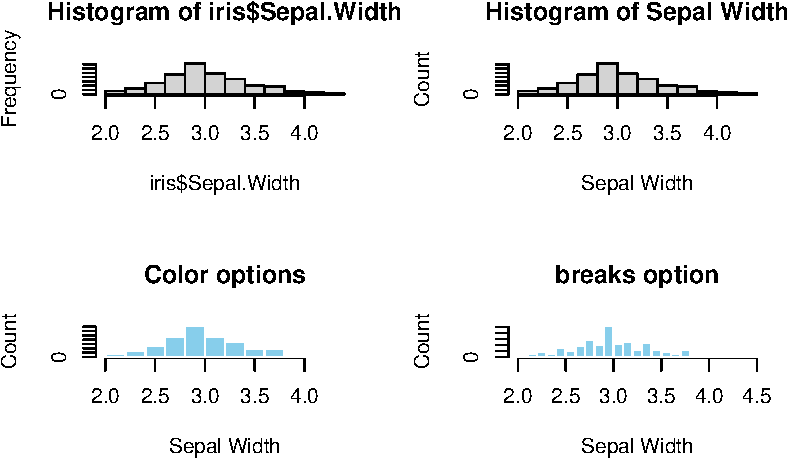
\includegraphics[keepaspectratio]{03_Data_Visualization_files/figure-pdf/fig-3-1-1.pdf}}

}

\caption{\label{fig-3-1}Base R Histogram. Top left: default. Top right:
Customized X-Y labels and the main title. Bottom left: change color of
bars and border. Bottom right: change the bin width (\texttt{breaks=})}

\end{figure}%

For the bottom-right graph, check out this line:
\texttt{breaks\ =\ seq(2,4.5,by=0.1)}. The aim is to customize the width
of the bars. The \texttt{seq()} function
(Section~\ref{sec-seq-function}) generates a list of numbers
(\texttt{2.0,\ 2.1\ ...\ 4.4,\ 4.5}) that represents the x-ticks.

Note: \texttt{par(mfrow=c(2,2))} splits the plotting area into a 2x2
grid such that multiple graphs can be displayed together. If you plot
contains only one graph, it can be ignored.

\subsubsection{Box Plot}\label{box-plot}

If robust statistics of the data is the message, the most appropriate
graph is a box plot. In a box plot, the y-axis represents the numeric
variable, and the x-axis has no meaning.

\begin{Shaded}
\begin{Highlighting}[]
\FunctionTok{par}\NormalTok{(}\AttributeTok{mfrow=}\FunctionTok{c}\NormalTok{(}\DecValTok{2}\NormalTok{,}\DecValTok{2}\NormalTok{))}

\CommentTok{\# Top left}
\FunctionTok{boxplot}\NormalTok{(iris}\SpecialCharTok{$}\NormalTok{Sepal.Width)}

\CommentTok{\# Top right}
\FunctionTok{boxplot}\NormalTok{(iris}\SpecialCharTok{$}\NormalTok{Sepal.Width,}
        \AttributeTok{ylab=}\StringTok{"Sepal Width"}\NormalTok{,}
        \AttributeTok{main=}\StringTok{"Box plot of Sepal Width"}\NormalTok{)}

\CommentTok{\# Bottom left}
\FunctionTok{boxplot}\NormalTok{(iris}\SpecialCharTok{$}\NormalTok{Sepal.Width,}
            \AttributeTok{col =} \StringTok{"skyblue"}\NormalTok{,}
            \AttributeTok{ylab=}\StringTok{"Sepal Width"}\NormalTok{,}
            \AttributeTok{outcol =} \StringTok{\textquotesingle{}red\textquotesingle{}}\NormalTok{,}
            \AttributeTok{outpch =} \DecValTok{19}\NormalTok{,}
            \AttributeTok{main=}\StringTok{"Color options"}\NormalTok{)}

\CommentTok{\# Bottom right}
\FunctionTok{boxplot}\NormalTok{(iris}\SpecialCharTok{$}\NormalTok{Sepal.Width, }
        \AttributeTok{horizontal =} \ConstantTok{TRUE}\NormalTok{, }
        \AttributeTok{xlab=}\StringTok{"Sepal Width"}\NormalTok{, }
        \AttributeTok{main=}\StringTok{"Horizontal Box plot"}\NormalTok{)}
\end{Highlighting}
\end{Shaded}

\begin{figure}[H]

\centering{

\pandocbounded{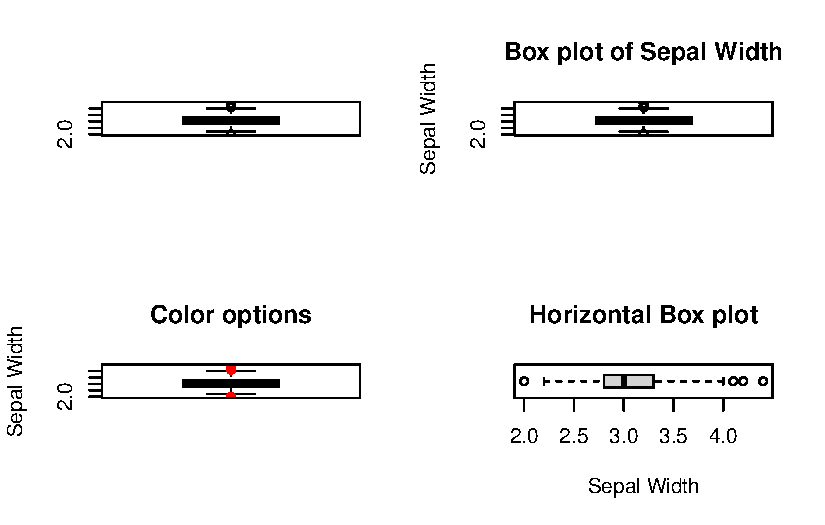
\includegraphics[keepaspectratio]{03_Data_Visualization_files/figure-pdf/fig-3-2-1.pdf}}

}

\caption{\label{fig-3-2}Base R Box plot. Top left: Default, Top right:
labels and main title. Bottom left: color options. Bottom right:
\texttt{horizontal\ =\ TRUE}}

\end{figure}%

\begin{figure}

\centering{

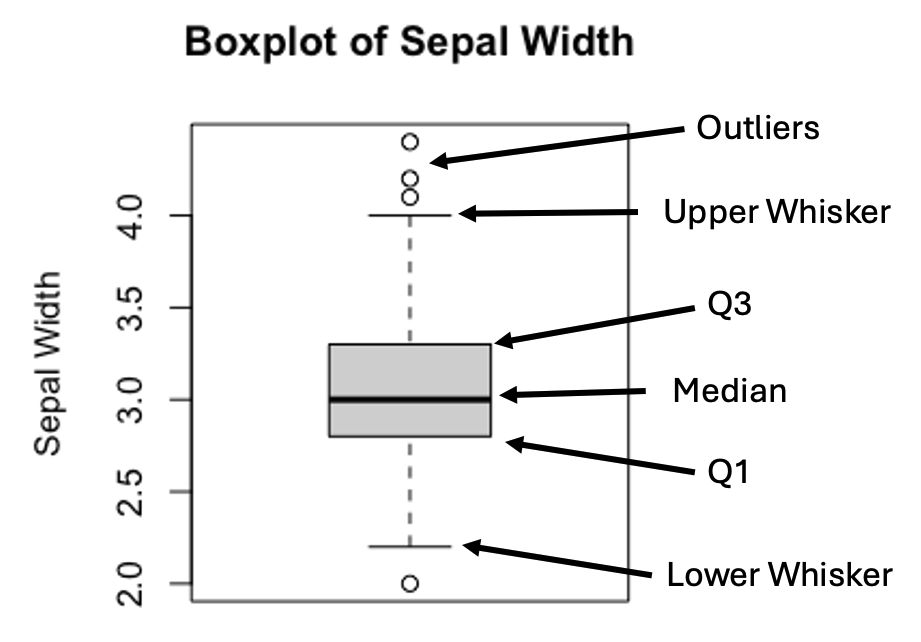
\includegraphics[width=0.6\linewidth,height=\textheight,keepaspectratio]{images/Figure_3.3.png}

}

\caption{\label{fig-3-3}Anatomy of a Box plot}

\end{figure}%

The upper and lower whiskers are defined as:

\[Upper\ Whisker = Q3 + 1.5 \times IQR\]
\[Lower\ Whisker = Q1 - 1.5 \times IQR\] , where \(IQR=(Q3-Q1)\).

As a practice, data points above the upper whisker or below the lower
whiskers are labeled as outliers.

While a box plot summarizes data into quartiles, a histogram portrays
the underlying distribution---such as peaks and symmetry---that is
otherwise difficult to spot. Is it a great idea to combine the best of
both plots in a single graph? To ensure that the combined plot makes
sense, we need to ensure that the axes of the two plots are in the same
range. Here's an example below:

\begin{Shaded}
\begin{Highlighting}[]
\FunctionTok{par}\NormalTok{(}\AttributeTok{mfrow=}\FunctionTok{c}\NormalTok{(}\DecValTok{2}\NormalTok{,}\DecValTok{1}\NormalTok{))}

\FunctionTok{hist}\NormalTok{(iris}\SpecialCharTok{$}\NormalTok{Sepal.Width, }
     \AttributeTok{breaks =} \FunctionTok{seq}\NormalTok{(}\DecValTok{2}\NormalTok{,}\FloatTok{4.5}\NormalTok{,}\AttributeTok{by=}\FloatTok{0.1}\NormalTok{), }
     \AttributeTok{col =} \StringTok{\textquotesingle{}skyblue\textquotesingle{}}\NormalTok{, }
     \AttributeTok{border =} \StringTok{\textquotesingle{}white\textquotesingle{}}\NormalTok{, }
     \AttributeTok{xlim =} \FunctionTok{c}\NormalTok{(}\DecValTok{2}\NormalTok{,}\FloatTok{4.5}\NormalTok{),}
     \AttributeTok{xlab =} \StringTok{""}\NormalTok{,}
     \AttributeTok{ylab =} \StringTok{"Count"}\NormalTok{, }
     \AttributeTok{main =} \StringTok{"Stacking Up Graphs"}\NormalTok{)}

\FunctionTok{boxplot}\NormalTok{(iris}\SpecialCharTok{$}\NormalTok{Sepal.Width, }
        \AttributeTok{horizontal =} \ConstantTok{TRUE}\NormalTok{, }
        \AttributeTok{ylim =} \FunctionTok{c}\NormalTok{(}\DecValTok{2}\NormalTok{,}\FloatTok{4.5}\NormalTok{),}
        \AttributeTok{xlab=}\StringTok{"Sepal Width"}\NormalTok{, }
        \AttributeTok{main=}\StringTok{""}\NormalTok{)}
\end{Highlighting}
\end{Shaded}

\begin{figure}[H]

\centering{

\pandocbounded{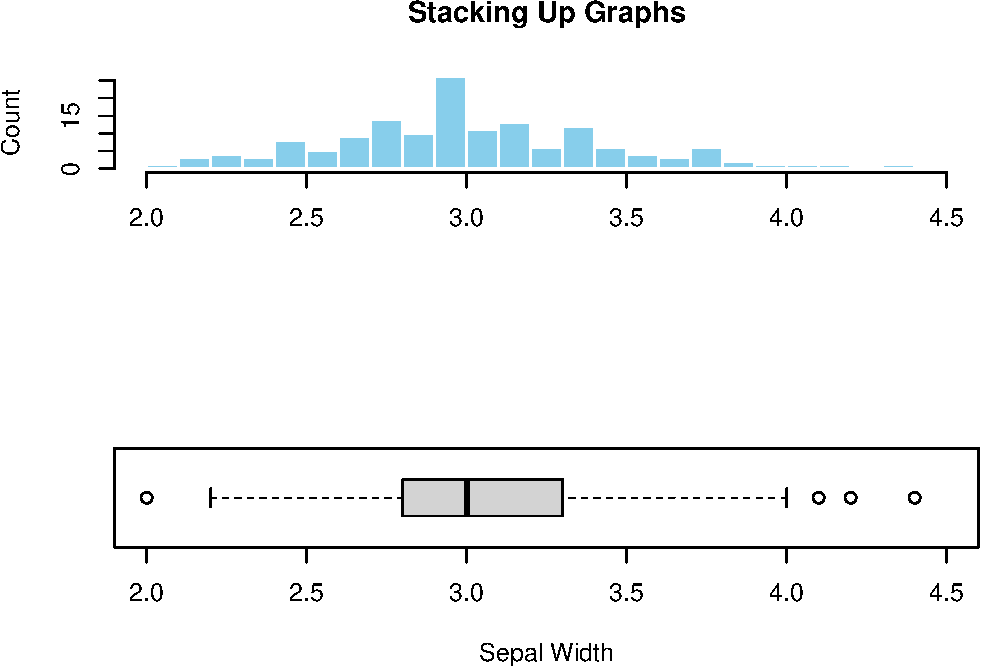
\includegraphics[keepaspectratio]{03_Data_Visualization_files/figure-pdf/fig-3-4-1.pdf}}

}

\caption{\label{fig-3-4}Stacking up a histogram and a box plot.}

\end{figure}%

The \texttt{ylim} of the histogram and the \texttt{xlim=} of the box
plot are the specific parameters used to align the two graphs in the
same scale.

Figure 3.4 illustrates the added advantage of combining graphs. It is
clear that the peak in the histogram is almost perfectly aligned with
the median shown in the box plot, suggesting the data distribution is
nearly symmetric. Additionally, the outliers, hardly visible in the
histogram, can easily be spotted in the box plot. This example
demonstrates the synergy offered by combining different types of graphs,
and the technique used to implement it.

\subsection{One Categorical Variable}\label{one-categorical-variable}

When it comes to categorical variables, we are usually interested in the
number of samples fall in each category of a categorical variable. As
discussed in Chapter~\ref{sec-02-data-wrangling}, the tallying can be
done using the \texttt{table()} function
(Section~\ref{sec-base-tabulation}) or \texttt{group\_by()} followed by
\texttt{summarize(n=n())} (Section~\ref{sec-tidyverse-tabulation}).

\subsubsection{Bar Plot}\label{bar-plot}

Bar plot is the standard choice for visualizing tallied data. The only
input to the R's \texttt{barplot()} graph function is a tabulated count
of the categorical variable. Here's an example:

\begin{Shaded}
\begin{Highlighting}[]
\FunctionTok{par}\NormalTok{(}\AttributeTok{mfrow=}\FunctionTok{c}\NormalTok{(}\DecValTok{2}\NormalTok{,}\DecValTok{2}\NormalTok{))}

\CommentTok{\# Top left}
\FunctionTok{barplot}\NormalTok{(}\FunctionTok{with}\NormalTok{(iris, }\FunctionTok{table}\NormalTok{(Species)))}

\CommentTok{\# Top right}
\FunctionTok{barplot}\NormalTok{(}\FunctionTok{with}\NormalTok{(iris, }\FunctionTok{table}\NormalTok{(Species)), }
        \AttributeTok{xlab=}\StringTok{"Species"}\NormalTok{, }
        \AttributeTok{ylab=}\StringTok{"Count"}\NormalTok{, }
        \AttributeTok{main=}\StringTok{"A Barplot of Species"}\NormalTok{)}

\CommentTok{\# Bottom left}
\FunctionTok{barplot}\NormalTok{(}\FunctionTok{with}\NormalTok{(iris, }\FunctionTok{table}\NormalTok{(Species)), }
        \AttributeTok{col=}\StringTok{\textquotesingle{}skyblue\textquotesingle{}}\NormalTok{, }
        \AttributeTok{border=}\StringTok{\textquotesingle{}blue\textquotesingle{}}\NormalTok{, }
        \AttributeTok{xlab=}\StringTok{"Species"}\NormalTok{, }
        \AttributeTok{ylab=}\StringTok{"Count"}\NormalTok{, }
        \AttributeTok{main=}\StringTok{"Color Options"}\NormalTok{)}

\CommentTok{\# Bottom right}
\FunctionTok{barplot}\NormalTok{(}\FunctionTok{with}\NormalTok{(iris, }\FunctionTok{table}\NormalTok{(Species)), }
        \AttributeTok{horiz =} \ConstantTok{TRUE}\NormalTok{, }
        \AttributeTok{col=}\StringTok{\textquotesingle{}skyblue\textquotesingle{}}\NormalTok{, }
        \AttributeTok{border=}\StringTok{\textquotesingle{}blue\textquotesingle{}}\NormalTok{, }
        \AttributeTok{xlab=}\StringTok{"Count"}\NormalTok{, }
        \AttributeTok{ylab=}\StringTok{"Species"}\NormalTok{, }
        \AttributeTok{main=}\StringTok{"A Horizontal Barplot"}\NormalTok{)}
\end{Highlighting}
\end{Shaded}

\begin{figure}[H]

\centering{

\pandocbounded{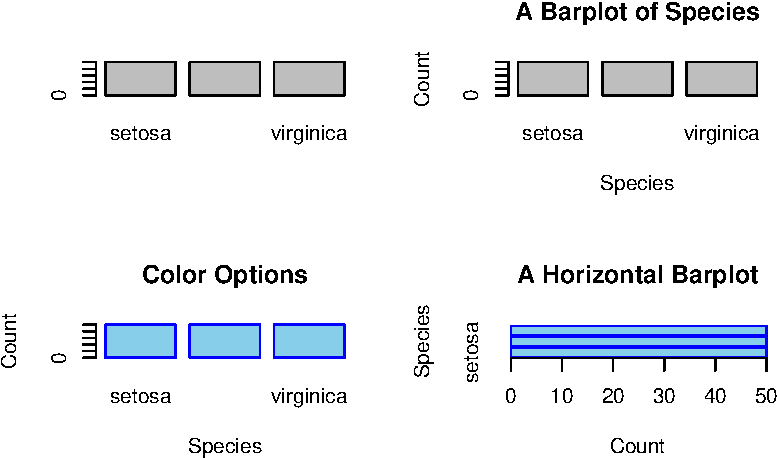
\includegraphics[keepaspectratio]{03_Data_Visualization_files/figure-pdf/fig-3-5-1.pdf}}

}

\caption{\label{fig-3-5}A simple bar plot. Top left: Default. Top right:
with tables}

\end{figure}%

Sometime you might want to reorder the categories along the x- or
y-axis. By default, \texttt{barplot()} places the bars from left to
right according to the order of the levels. E.g., show the levels of
\texttt{iris\$Species} by:

\begin{Shaded}
\begin{Highlighting}[]
\FunctionTok{levels}\NormalTok{(iris}\SpecialCharTok{$}\NormalTok{Species)}
\end{Highlighting}
\end{Shaded}

\begin{verbatim}
[1] "setosa"     "versicolor" "virginica" 
\end{verbatim}

You can change the order of the levels by updating the factor variable
using the \texttt{factor()} function (Section~\ref{sec-factor-levels}).
Suppose, the desired order is \texttt{virginica}, \texttt{setosa}, and
\texttt{veriscolor}. Here's the code:

\begin{Shaded}
\begin{Highlighting}[]
\NormalTok{iris}\SpecialCharTok{$}\NormalTok{Species }\OtherTok{\textless{}{-}} \FunctionTok{factor}\NormalTok{(iris}\SpecialCharTok{$}\NormalTok{Species, }
                       \AttributeTok{levels =} \FunctionTok{c}\NormalTok{(}\StringTok{"virginica"}\NormalTok{, }\StringTok{"setosa"}\NormalTok{, }\StringTok{"versicolor"}\NormalTok{), }
                       \AttributeTok{ordered =} \ConstantTok{TRUE}\NormalTok{)}
\FunctionTok{levels}\NormalTok{(iris}\SpecialCharTok{$}\NormalTok{Species)}
\end{Highlighting}
\end{Shaded}

\begin{verbatim}
[1] "virginica"  "setosa"     "versicolor"
\end{verbatim}

Here's the revised bar plot.

\begin{Shaded}
\begin{Highlighting}[]
\FunctionTok{barplot}\NormalTok{(}\FunctionTok{with}\NormalTok{(iris, }\FunctionTok{table}\NormalTok{(Species)), }
        \AttributeTok{col=}\StringTok{\textquotesingle{}skyblue\textquotesingle{}}\NormalTok{, }
        \AttributeTok{border=}\StringTok{\textquotesingle{}blue\textquotesingle{}}\NormalTok{, }
        \AttributeTok{xlab=}\StringTok{"Species"}\NormalTok{, }
        \AttributeTok{ylab=}\StringTok{"Count"}\NormalTok{, }
        \AttributeTok{main=}\StringTok{"Reordered Species"}\NormalTok{)}
\end{Highlighting}
\end{Shaded}

\begin{figure}[H]

\centering{

\pandocbounded{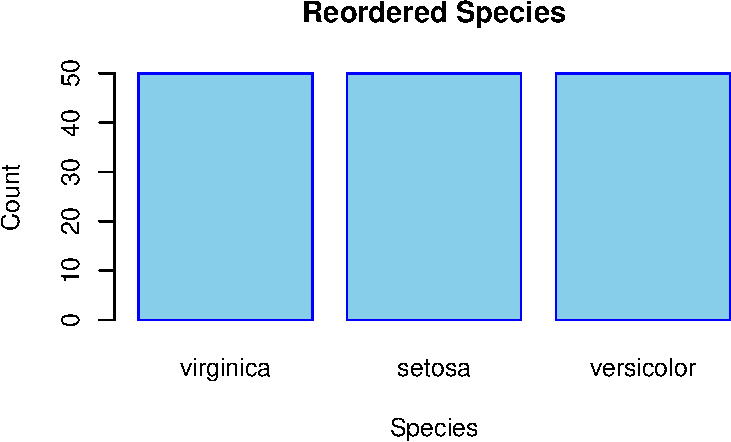
\includegraphics[keepaspectratio]{03_Data_Visualization_files/figure-pdf/fig-3-6-1.pdf}}

}

\caption{\label{fig-3-6}Reorder the Bars of a Barplot}

\end{figure}%

\subsubsection{Pie Chart}\label{pie-chart}

An alternative to bar plots is pie charts.

\begin{Shaded}
\begin{Highlighting}[]
\FunctionTok{par}\NormalTok{(}\AttributeTok{mfrow=}\FunctionTok{c}\NormalTok{(}\DecValTok{2}\NormalTok{,}\DecValTok{2}\NormalTok{))}

\CommentTok{\# Top left}
\FunctionTok{pie}\NormalTok{(}\FunctionTok{with}\NormalTok{(iris, }\FunctionTok{table}\NormalTok{(Species)))}

\CommentTok{\# Top left}
\FunctionTok{pie}\NormalTok{(}\FunctionTok{with}\NormalTok{(iris, }\FunctionTok{table}\NormalTok{(Species)), }
    \AttributeTok{col =} \FunctionTok{c}\NormalTok{(}\StringTok{\textquotesingle{}skyblue\textquotesingle{}}\NormalTok{, }\StringTok{\textquotesingle{}orange\textquotesingle{}}\NormalTok{, }\StringTok{\textquotesingle{}white\textquotesingle{}}\NormalTok{), }
    \AttributeTok{main=}\StringTok{"Species"}\NormalTok{)}

\CommentTok{\# Bottom right}
\NormalTok{counts }\OtherTok{\textless{}{-}} \FunctionTok{with}\NormalTok{(iris, }\FunctionTok{table}\NormalTok{(Species))}
\NormalTok{my\_labs }\OtherTok{\textless{}{-}} \FunctionTok{paste0}\NormalTok{(}\FunctionTok{names}\NormalTok{(counts),}\StringTok{"("}\NormalTok{,counts,}\StringTok{")"}\NormalTok{)}
\FunctionTok{pie}\NormalTok{(counts, }
    \AttributeTok{labels =}\NormalTok{ my\_labs, }
    \AttributeTok{col =} \FunctionTok{c}\NormalTok{(}\StringTok{\textquotesingle{}skyblue\textquotesingle{}}\NormalTok{, }\StringTok{\textquotesingle{}orange\textquotesingle{}}\NormalTok{, }\StringTok{\textquotesingle{}white\textquotesingle{}}\NormalTok{), }
    \AttributeTok{main =} \StringTok{"Species Counts"}\NormalTok{)}


\CommentTok{\# Bottom right}
\NormalTok{counts }\OtherTok{\textless{}{-}} \FunctionTok{with}\NormalTok{(iris, }\FunctionTok{table}\NormalTok{(Species))}
\NormalTok{fractions }\OtherTok{\textless{}{-}} \FunctionTok{round}\NormalTok{(counts}\SpecialCharTok{/}\FunctionTok{sum}\NormalTok{(counts),}\DecValTok{2}\NormalTok{)}
\NormalTok{my\_labs }\OtherTok{\textless{}{-}} \FunctionTok{paste0}\NormalTok{(}\FunctionTok{names}\NormalTok{(counts),}\StringTok{"("}\NormalTok{,fractions,}\StringTok{")"}\NormalTok{)}
\FunctionTok{pie}\NormalTok{(counts, }
    \AttributeTok{labels =}\NormalTok{ my\_labs, }
    \AttributeTok{col =} \FunctionTok{c}\NormalTok{(}\StringTok{\textquotesingle{}skyblue\textquotesingle{}}\NormalTok{, }\StringTok{\textquotesingle{}orange\textquotesingle{}}\NormalTok{, }\StringTok{\textquotesingle{}white\textquotesingle{}}\NormalTok{), }
    \AttributeTok{main =} \StringTok{"Species Fractions"}\NormalTok{)}
\end{Highlighting}
\end{Shaded}

\begin{figure}[H]

\centering{

\pandocbounded{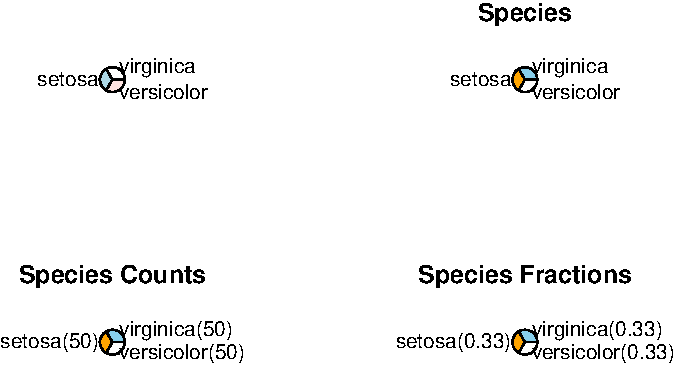
\includegraphics[keepaspectratio]{03_Data_Visualization_files/figure-pdf/fig-3-7-1.pdf}}

}

\caption{\label{fig-3-7}A simple pie chart. Top left: Default. Top
right: with tables. Bottom left: Add a title. Show count for each
category. Bottom right: Add a fraction or proportion for each category.}

\end{figure}%

\subsection{One Categorical and One Numeric
Variables}\label{one-categorical-and-one-numeric-variables}

The categorical variable in this situation is usually served as a group
identifier that splits the data into groups so the numerical variable
can be compared between groups. This kind of graph is generally named
\textbf{side-by-side plot}. You can choose a side-by-side box plot or a
side-by-side bar plot. For example, a side-by-side box plot that
visually compares the robust statistics of \texttt{Sepal.Length} between
different species of iris.

\subsubsection{Side-by-side box plot}\label{side-by-side-box-plot}

\begin{Shaded}
\begin{Highlighting}[]
\FunctionTok{par}\NormalTok{(}\AttributeTok{mfrow=}\FunctionTok{c}\NormalTok{(}\DecValTok{2}\NormalTok{,}\DecValTok{1}\NormalTok{))}

\FunctionTok{boxplot}\NormalTok{(Sepal.Length }\SpecialCharTok{\textasciitilde{}}\NormalTok{ Species,}
        \AttributeTok{data=}\NormalTok{iris, }
        \AttributeTok{main=}\StringTok{"A Side{-}by{-}Side Box plot"}\NormalTok{)}

\FunctionTok{boxplot}\NormalTok{(Sepal.Length }\SpecialCharTok{\textasciitilde{}}\NormalTok{ Species,}
        \AttributeTok{data=}\NormalTok{iris, }
        \AttributeTok{horizontal =} \ConstantTok{TRUE}\NormalTok{,}
        \AttributeTok{main=}\StringTok{"A Horizontal Side{-}by{-}Side Box plot"}\NormalTok{)}
\end{Highlighting}
\end{Shaded}

\begin{figure}[H]

\centering{

\pandocbounded{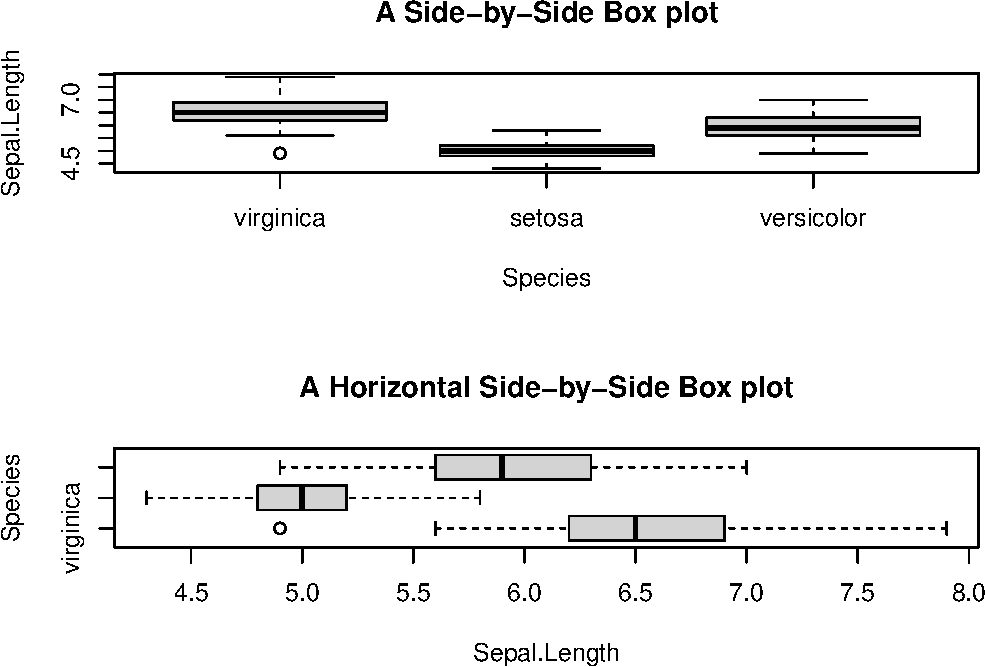
\includegraphics[keepaspectratio]{03_Data_Visualization_files/figure-pdf/fig-3-8-1.pdf}}

}

\caption{\label{fig-3-8}A side-by-side box plot}

\end{figure}%

\texttt{Sepal.Length\ \textasciitilde{}\ Species} is read as ``Sepal
length \textbf{by} species'', the tilde symbol
``\texttt{\textasciitilde{}}'' means ``by''.

However, there is glitch in the horizontal box plot (bottom): the
y-labels collide. It can be fixed by:

\begin{enumerate}
\def\labelenumi{\arabic{enumi}.}
\item
  Expand the left margin of the plotting area.
\item
  Add the \texttt{las=2} parameter to the \texttt{boxplot()} function,
  and disable the default \texttt{ylab=}.
\item
  Mannually add the y-label.
\end{enumerate}

\begin{Shaded}
\begin{Highlighting}[]
\CommentTok{\# Expand the left margin so the text doesn\textquotesingle{}t truncate}
\CommentTok{\# The numbers correspond to margins: c(bottom, left, top, right)}
\CommentTok{\# Default is c(5, 4, 4, 2). We are increasing the left margin from 4 to 7. }
\FunctionTok{par}\NormalTok{(}\AttributeTok{mar =} \FunctionTok{c}\NormalTok{(}\DecValTok{5}\NormalTok{, }\DecValTok{7}\NormalTok{, }\DecValTok{4}\NormalTok{, }\DecValTok{2}\NormalTok{) }\SpecialCharTok{+} \FloatTok{0.1}\NormalTok{)}

\CommentTok{\# Draw the plot, but explicitly tell R NOT to draw the y{-}axis label yet}
\FunctionTok{boxplot}\NormalTok{(Sepal.Length }\SpecialCharTok{\textasciitilde{}}\NormalTok{ Species,}
        \AttributeTok{data=}\NormalTok{iris, }
        \AttributeTok{horizontal =} \ConstantTok{TRUE}\NormalTok{,}
        \AttributeTok{las =} \DecValTok{2}\NormalTok{,}
        \AttributeTok{ylab =} \StringTok{""}\NormalTok{, }\CommentTok{\# This suppresses the default colliding label}
        \AttributeTok{main=}\StringTok{"Y{-}tick Labels Reorientated"}\NormalTok{)}

\CommentTok{\# Add the y{-}axis label manually, pushing it further away from the axis}
\CommentTok{\# The \textquotesingle{}line\textquotesingle{} argument controls how many text lines away from the axis it sits}
\FunctionTok{title}\NormalTok{(}\AttributeTok{ylab =} \StringTok{"Species"}\NormalTok{, }\AttributeTok{line =} \DecValTok{5}\NormalTok{)}
\end{Highlighting}
\end{Shaded}

\begin{figure}[H]

\centering{

\pandocbounded{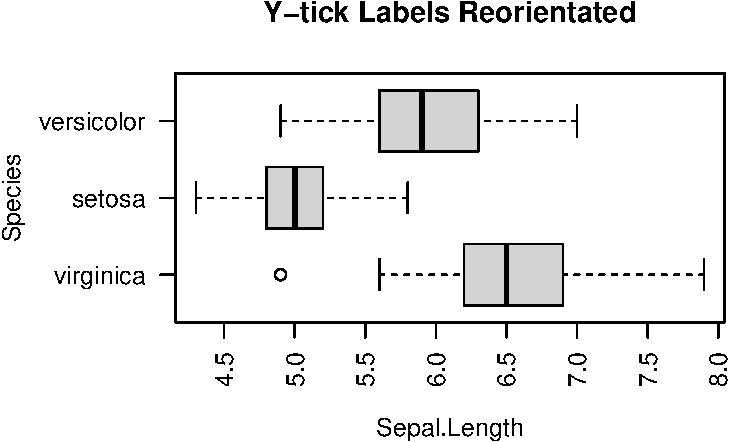
\includegraphics[keepaspectratio]{03_Data_Visualization_files/figure-pdf/fig-3-9-1.pdf}}

}

\caption{\label{fig-3-9}A Side-by-Side Box Plot with Horizontal
Y-Labels}

\end{figure}%

\subsubsection{Side-by-side Bar Plot}\label{side-by-side-bar-plot}

Suppose you want to visually compare the average sepal length among
different iris species. You will begin to feel the cumbersome of base R,
and appreciate the power of \texttt{tidyverse}. Anyway, you will see how
to make such a graph with a new function, \texttt{tapply()}, in two
steps.

First, make a table of average sepal length by species. Apparently, the
\texttt{table()} function may help. But it does not work for this case,
as it only tallies the number of samples by species. Hence, you need to
use a new function \texttt{tapply()}. Here's an example:

\begin{Shaded}
\begin{Highlighting}[]
\NormalTok{mean\_data }\OtherTok{\textless{}{-}} \FunctionTok{tapply}\NormalTok{(iris}\SpecialCharTok{$}\NormalTok{Sepal.Length, iris}\SpecialCharTok{$}\NormalTok{Species, }\AttributeTok{FUN =}\NormalTok{ mean)}
\NormalTok{mean\_data}
\end{Highlighting}
\end{Shaded}

\begin{verbatim}
 virginica     setosa versicolor 
     6.588      5.006      5.936 
\end{verbatim}

How does \texttt{tapply()} work? The ``\texttt{t}'' represents table.
The function applies the \texttt{mean} function to the input data
\texttt{iris\$Sepal.Length} grouped by \texttt{iris\$Species}. In other
words, the \texttt{mean()} is applied to the sepal lengths for each
species separately.

And then, pass the \texttt{mean\_data} object to \texttt{barplot()}.

\begin{Shaded}
\begin{Highlighting}[]
\FunctionTok{barplot}\NormalTok{(mean\_data,}
        \AttributeTok{xlab=}\StringTok{"Species"}\NormalTok{, }
        \AttributeTok{ylab=}\StringTok{"Average Sepal.Length"}\NormalTok{, }
        \AttributeTok{main=}\StringTok{"Side{-}by{-}side Barplot"}\NormalTok{)}
\end{Highlighting}
\end{Shaded}

\begin{figure}[H]

\centering{

\pandocbounded{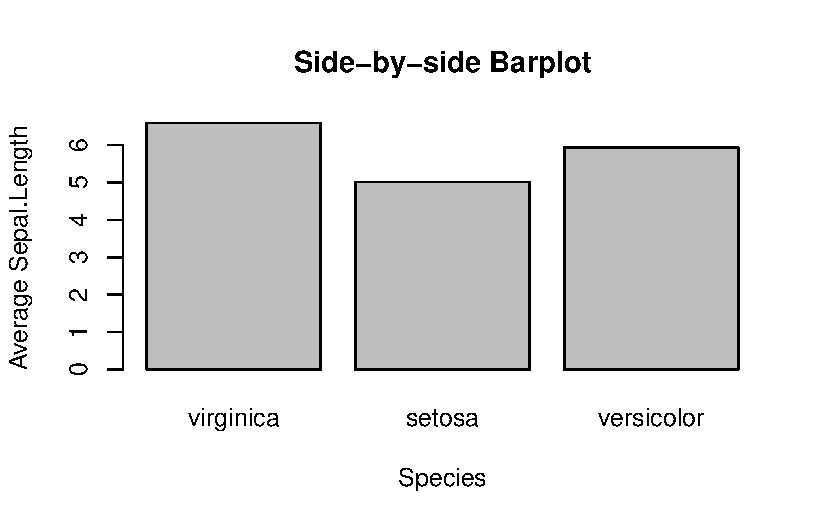
\includegraphics[keepaspectratio]{03_Data_Visualization_files/figure-pdf/fig-3-10-1.pdf}}

}

\caption{\label{fig-3-10}A Side-by-Side Bar Plot}

\end{figure}%

\subsubsection{Side-by-side Bar Plot with Error
Bar\^{}*}\label{side-by-side-bar-plot-with-error-bar}

\emph{This topic is slightly advanced. It is much easier to use
\texttt{ggplot2}. So, feel free to skip this or jump to
Section~\ref{sec-ggplot-error-bar}.}

The error bar represents the standard error of the mean (SEM). Here is
the formula:

\[\huge{\bar{x}\pm\frac{s}{\sqrt{n}}}\] , where \(s\) and \(n\) are the
standard deviation and sample size, respectively. In the bar plot you
are going to plot, the height of the bar is \(\bar{x}\), and the error
bars span above and below the bar's top by \(\frac{s}{\sqrt{n}}\) units.

First, calculate the mean and standard of errors using the
\texttt{tapply()} function.

\begin{Shaded}
\begin{Highlighting}[]
\NormalTok{mean\_data }\OtherTok{\textless{}{-}} \FunctionTok{tapply}\NormalTok{(iris}\SpecialCharTok{$}\NormalTok{Sepal.Length, iris}\SpecialCharTok{$}\NormalTok{Species, }\AttributeTok{FUN =}\NormalTok{ mean)}
\NormalTok{mean\_data}
\end{Highlighting}
\end{Shaded}

\begin{verbatim}
 virginica     setosa versicolor 
     6.588      5.006      5.936 
\end{verbatim}

\begin{Shaded}
\begin{Highlighting}[]
\NormalTok{sem }\OtherTok{\textless{}{-}} \ControlFlowTok{function}\NormalTok{(x) \{}\FunctionTok{sd}\NormalTok{(x)}\SpecialCharTok{/}\FunctionTok{sqrt}\NormalTok{(}\FunctionTok{length}\NormalTok{(x))\}}
\NormalTok{sem\_data }\OtherTok{\textless{}{-}} \FunctionTok{tapply}\NormalTok{(iris}\SpecialCharTok{$}\NormalTok{Sepal.Length, iris}\SpecialCharTok{$}\NormalTok{Species, }\AttributeTok{FUN =}\NormalTok{ sem)}
\NormalTok{sem\_data}
\end{Highlighting}
\end{Shaded}

\begin{verbatim}
 virginica     setosa versicolor 
0.08992695 0.04984957 0.07299762 
\end{verbatim}

First, create the bar plot and store the height of bars in the object
\texttt{bar\_midpoints}. Use the \texttt{arrows()} function to
create/add the error bars to the bar plot, where each error bar consists
of the upper whisker \((x_{1}, y_{1})\) and lower whisker
\((x_{0}, y_{0})\).

\begin{Shaded}
\begin{Highlighting}[]
\NormalTok{bar\_midpoints }\OtherTok{\textless{}{-}} \FunctionTok{barplot}\NormalTok{(mean\_data,}
                  \AttributeTok{xlab=}\StringTok{"Species"}\NormalTok{, }
                  \AttributeTok{ylab=}\StringTok{"Average Sepal.Length"}\NormalTok{, }
                  \AttributeTok{main=}\StringTok{"Side{-}by{-}side Barplot"}\NormalTok{)}

\FunctionTok{arrows}\NormalTok{(}\AttributeTok{x0 =}\NormalTok{ bar\_midpoints,}
       \AttributeTok{y0 =}\NormalTok{ mean\_data }\SpecialCharTok{{-}}\NormalTok{ sem\_data, }\CommentTok{\# Start of the bar}
       \AttributeTok{x1 =}\NormalTok{ bar\_midpoints,}
       \AttributeTok{y1 =}\NormalTok{ mean\_data }\SpecialCharTok{+}\NormalTok{ sem\_data, }\CommentTok{\# End of the bar}
       \AttributeTok{angle =} \DecValTok{90}\NormalTok{,                }\CommentTok{\# Makes the ends of the bars flat}
       \AttributeTok{code =} \DecValTok{3}\NormalTok{,                  }\CommentTok{\# Draws ticks at both ends}
       \AttributeTok{length =} \FloatTok{0.5}\NormalTok{, }\AttributeTok{col=}\StringTok{\textquotesingle{}red\textquotesingle{}}\NormalTok{)   }\CommentTok{\# Sets the length of the ticks}
\end{Highlighting}
\end{Shaded}

\begin{figure}[H]

\centering{

\pandocbounded{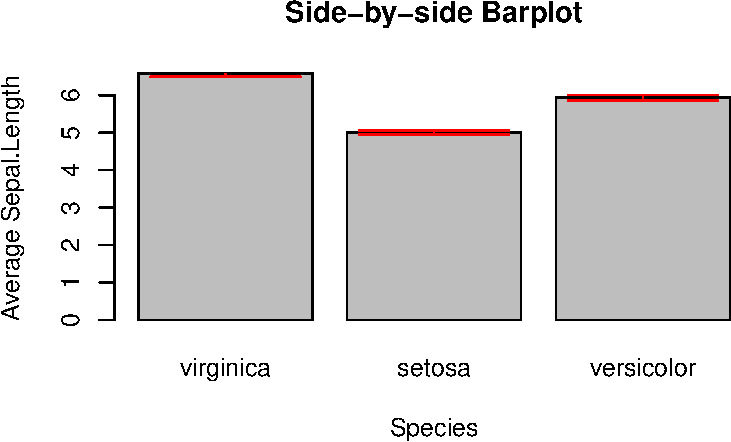
\includegraphics[keepaspectratio]{03_Data_Visualization_files/figure-pdf/fig-3-11-1.pdf}}

}

\caption{\label{fig-3-11}A Side-by-side Bar Plot with Error Bars}

\end{figure}%

Once again, if you found this confusing, see the \texttt{ggplot} version
of error bars (Section~\ref{sec-ggplot-error-bar}).

\subsubsection{Line Graph with Error
Bar}\label{line-graph-with-error-bar}

If your message is to show a trend from left to right, a line graph is
the default choice. Here is an example to create a line graph with solid
dots.

\begin{Shaded}
\begin{Highlighting}[]
\CommentTok{\# Default line plot}
\FunctionTok{plot}\NormalTok{(mean\_data,}
      \AttributeTok{type=}\StringTok{\textquotesingle{}b\textquotesingle{}}\NormalTok{,}
      \AttributeTok{pch=}\DecValTok{19}\NormalTok{,}
      \AttributeTok{xlab=}\StringTok{"Species"}\NormalTok{,}
      \AttributeTok{ylab=}\StringTok{"Average Sepal.Length"}\NormalTok{,}
      \AttributeTok{main=}\StringTok{"A Line Plot"}\NormalTok{)}
\end{Highlighting}
\end{Shaded}

\begin{figure}[H]

\centering{

\pandocbounded{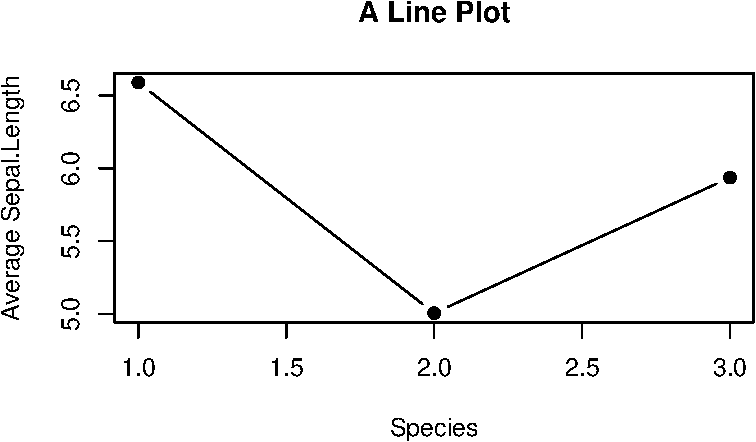
\includegraphics[keepaspectratio]{03_Data_Visualization_files/figure-pdf/fig-3-12-1.pdf}}

}

\caption{\label{fig-3-12}A Line Plot}

\end{figure}%

\begin{itemize}
\item
  Use \texttt{pch=19} to specify the shape of the data points.
  \texttt{pch} stands for \textbf{p}lotting \textbf{ch}aracter. The
  value \texttt{19} denotes a solid dot (\(\bullet\)).
\item
  To join the dots together in a line plot, specify
  \texttt{type=\textquotesingle{}b\textquotesingle{}}, the \texttt{b}
  means \textbf{both} dots and line are plotted. More options of
  \texttt{type} can be found using the help function:
  \texttt{help(plot)} documentation.
\end{itemize}

But, there is a glitch in the x-tick.The x-tick should show the actual
species names instead of number. It can be fixed in two steps: 1.
Suppress the default x-tick labeling feature of the \texttt{plot()}
function by setting the parameter \texttt{xaxt="n"}. And then, paste the
customized x-tick back by the \texttt{axis()} function. The species
names can be obtained by \texttt{names(mean\_data)}.

\begin{Shaded}
\begin{Highlighting}[]
\CommentTok{\# Fix x{-}tick labels}
\FunctionTok{plot}\NormalTok{(mean\_data,}
      \AttributeTok{type=}\StringTok{\textquotesingle{}b\textquotesingle{}}\NormalTok{,}
      \AttributeTok{pch=}\DecValTok{19}\NormalTok{,}
      \AttributeTok{xlab=}\StringTok{"Species"}\NormalTok{,}
      \AttributeTok{ylab=}\StringTok{"Average Sepal.Length"}\NormalTok{,}
      \AttributeTok{main=}\StringTok{"Change x{-}tick Labels"}\NormalTok{,}
      \AttributeTok{xaxt=}\StringTok{"n"}\NormalTok{)}
\FunctionTok{axis}\NormalTok{(}\AttributeTok{side=}\DecValTok{1}\NormalTok{, }\AttributeTok{at=}\DecValTok{1}\SpecialCharTok{:}\FunctionTok{length}\NormalTok{(mean\_data), }\AttributeTok{labels=}\FunctionTok{names}\NormalTok{(mean\_data))}
\end{Highlighting}
\end{Shaded}

\begin{figure}[H]

\centering{

\pandocbounded{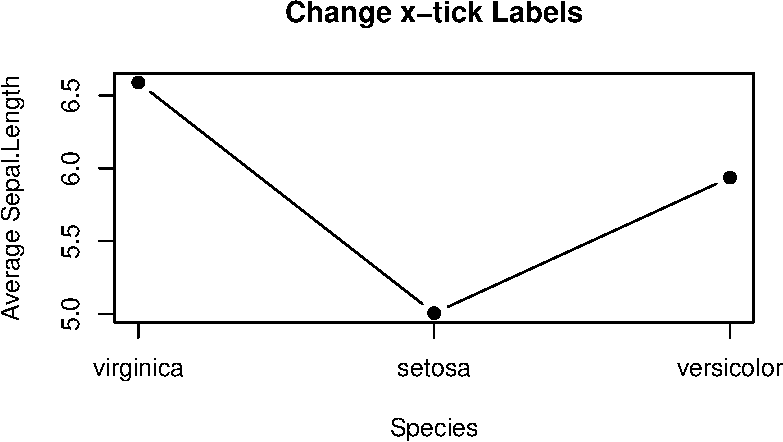
\includegraphics[keepaspectratio]{03_Data_Visualization_files/figure-pdf/fig-3-13-1.pdf}}

}

\caption{\label{fig-3-13}A Line plot with proper x-tick labels}

\end{figure}%

Now we can add error bars to the line plot. It is similar to the bar
plot above, except that \texttt{x0} and \texttt{x1} should take the
values \texttt{1,2,3}.

\begin{Shaded}
\begin{Highlighting}[]
\CommentTok{\# Add Error Bar}
\FunctionTok{plot}\NormalTok{(mean\_data,}
      \AttributeTok{type=}\StringTok{\textquotesingle{}b\textquotesingle{}}\NormalTok{,}
      \AttributeTok{pch=}\DecValTok{19}\NormalTok{,}
      \AttributeTok{xlab=}\StringTok{"Species"}\NormalTok{, }
      \AttributeTok{ylab=}\StringTok{"Average Sepal.Length"}\NormalTok{, }
      \AttributeTok{main=}\StringTok{"Change x{-}tick Labels"}\NormalTok{,}
      \AttributeTok{xaxt=}\StringTok{"n"}\NormalTok{)}
\FunctionTok{axis}\NormalTok{(}\AttributeTok{side=}\DecValTok{1}\NormalTok{, }\AttributeTok{at=}\DecValTok{1}\SpecialCharTok{:}\FunctionTok{length}\NormalTok{(mean\_data), }\AttributeTok{labels=}\FunctionTok{names}\NormalTok{(mean\_data))}

\FunctionTok{arrows}\NormalTok{(}\AttributeTok{x0 =} \FunctionTok{seq}\NormalTok{(}\FunctionTok{length}\NormalTok{(mean\_data)),}
       \AttributeTok{y0 =}\NormalTok{ mean\_data }\SpecialCharTok{{-}}\NormalTok{ sem\_data, }\CommentTok{\# Start of the bar}
       \AttributeTok{x1 =} \FunctionTok{seq}\NormalTok{(}\FunctionTok{length}\NormalTok{(mean\_data)),}
       \AttributeTok{y1 =}\NormalTok{ mean\_data }\SpecialCharTok{+}\NormalTok{ sem\_data, }\CommentTok{\# End of the bar}
       \AttributeTok{angle =} \DecValTok{90}\NormalTok{,                }\CommentTok{\# Makes the ends of the bars flat}
       \AttributeTok{code =} \DecValTok{3}\NormalTok{,                  }\CommentTok{\# Draws ticks at both ends}
       \AttributeTok{length =} \FloatTok{0.05}\NormalTok{, }\AttributeTok{col=}\StringTok{\textquotesingle{}red\textquotesingle{}}\NormalTok{)   }\CommentTok{\# Sets the length of the ticks}
\end{Highlighting}
\end{Shaded}

\begin{figure}[H]

\centering{

\pandocbounded{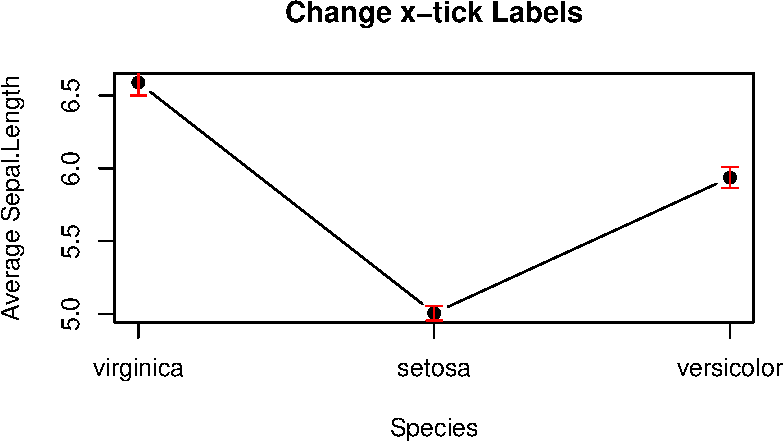
\includegraphics[keepaspectratio]{03_Data_Visualization_files/figure-pdf/fig-3-14-1.pdf}}

}

\caption{\label{fig-3-14}A Line plot with Error Bars}

\end{figure}%

\subsubsection{Overlapping Histogram}\label{overlapping-histogram}

\emph{The code for creating this plot can be convoluted. It is easier to
make it using \texttt{ggplot2}. Feel free to skip to
Section~\ref{sec-ggplot-overlapping-histogram}.}

Suppose you are interested in visualizing and comparing the distribution
of sepal lengths among the three iris species. Here are the steps to do
it:

\begin{enumerate}
\def\labelenumi{\arabic{enumi}.}
\item
  Split the data by individual species.
\item
  Calculate the range for the x- and y-axis so as to ensure the
  histograms are in the same scale.
\item
  Create a histogram in certain color for a species from step 1, and use
  it as a template.
\item
  Overlay the histograms from other species on top of each other.
\end{enumerate}

Let's do it step by step below:

\begin{Shaded}
\begin{Highlighting}[]
\CommentTok{\# Step 1: Split the data by individual species}

\NormalTok{setosa }\OtherTok{\textless{}{-}} \FunctionTok{subset}\NormalTok{(iris, Species }\SpecialCharTok{==} \StringTok{"setosa"}\NormalTok{)}
\NormalTok{versicolor }\OtherTok{\textless{}{-}} \FunctionTok{subset}\NormalTok{(iris, Species }\SpecialCharTok{==} \StringTok{"versicolor"}\NormalTok{)}
\NormalTok{virginica }\OtherTok{\textless{}{-}} \FunctionTok{subset}\NormalTok{(iris, Species }\SpecialCharTok{==} \StringTok{"virginica"}\NormalTok{)}
\end{Highlighting}
\end{Shaded}

\begin{Shaded}
\begin{Highlighting}[]
\CommentTok{\# Step 2: Set up the range for the x{-} and y{-}axis}

\NormalTok{x\_range }\OtherTok{\textless{}{-}} \FunctionTok{range}\NormalTok{(iris}\SpecialCharTok{$}\NormalTok{Sepal.Length)}
\NormalTok{y\_range }\OtherTok{\textless{}{-}} \FunctionTok{c}\NormalTok{(}\DecValTok{0}\NormalTok{, }\DecValTok{25}\NormalTok{) }\CommentTok{\# 25 is arbitrary.}
\end{Highlighting}
\end{Shaded}

Below is the code for plotting the template histogram, and how
additional histograms are added to it. To distinguish species, different
color is attributed to different species. It is done by
\texttt{col\ =\ rgb(...)}. The \texttt{rgb()} function stands for
\textbf{r}ed, \textbf{g}reen, and \textbf{b}lue. It takes four
parameters: the intensity of red, green, blue, and transparency. All are
in the range of 0 and 1. E.g., \texttt{rgb(1,\ 0,\ 0,\ 0.5)} means 100\%
red, no green and blue at all, and transparency is 50\%.

\begin{Shaded}
\begin{Highlighting}[]
\CommentTok{\# Step 3: Create a template}

\FunctionTok{hist}\NormalTok{(setosa}\SpecialCharTok{$}\NormalTok{Sepal.Length,}
     \AttributeTok{main =} \StringTok{"Overlapping Histogram of Sepal Length"}\NormalTok{,}
     \AttributeTok{xlab =} \StringTok{"Sepal Length"}\NormalTok{,}
     \AttributeTok{col =} \FunctionTok{rgb}\NormalTok{(}\DecValTok{1}\NormalTok{, }\DecValTok{0}\NormalTok{, }\DecValTok{0}\NormalTok{, }\FloatTok{0.5}\NormalTok{), }\CommentTok{\# Red with 50\% transparency}
     \AttributeTok{breaks =} \FunctionTok{seq}\NormalTok{(}\DecValTok{4}\NormalTok{,}\DecValTok{9}\NormalTok{,}\AttributeTok{by=}\FloatTok{0.25}\NormalTok{),}
     \AttributeTok{xlim =}\NormalTok{ x\_range,}
     \AttributeTok{ylim =}\NormalTok{ y\_range)}

\CommentTok{\# Step 4: Overlay histograms from other species}

\FunctionTok{hist}\NormalTok{(versicolor}\SpecialCharTok{$}\NormalTok{Sepal.Length, }\AttributeTok{col=}\FunctionTok{rgb}\NormalTok{(}\DecValTok{0}\NormalTok{, }\DecValTok{1}\NormalTok{, }\DecValTok{0}\NormalTok{, }\FloatTok{0.5}\NormalTok{), }\AttributeTok{add =} \ConstantTok{TRUE}\NormalTok{) }\CommentTok{\# green with 50\% transparency}
\FunctionTok{hist}\NormalTok{(virginica}\SpecialCharTok{$}\NormalTok{Sepal.Length, }\AttributeTok{col=}\FunctionTok{rgb}\NormalTok{(}\DecValTok{0}\NormalTok{, }\DecValTok{0}\NormalTok{, }\DecValTok{1}\NormalTok{, }\FloatTok{0.5}\NormalTok{), }\AttributeTok{add =} \ConstantTok{TRUE}\NormalTok{)  }\CommentTok{\# blue with 50\% transparency}
\end{Highlighting}
\end{Shaded}

\begin{figure}[H]

\centering{

\pandocbounded{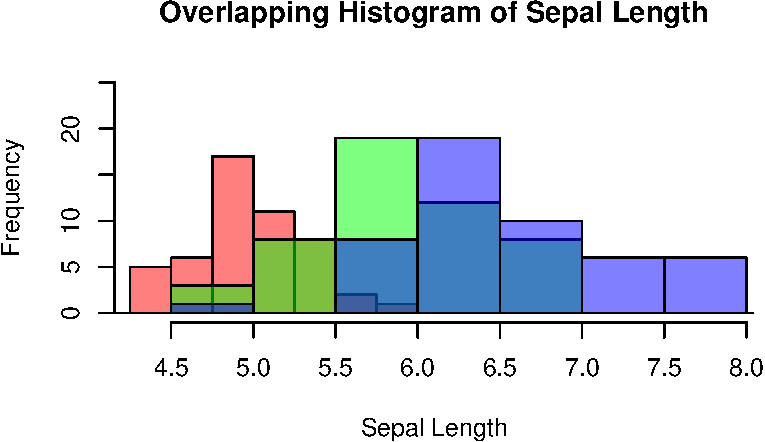
\includegraphics[keepaspectratio]{03_Data_Visualization_files/figure-pdf/fig-3-15-1.pdf}}

}

\caption{\label{fig-3-15}Overlapping histograms}

\end{figure}%

\subsection{Contingency Table}\label{contingency-table}

Here we deal with a data set that comprises two categorical variables. A
two-dimensional contingency table is used to tally the number of samples
for different combinations of categories of the two categorical
variables.

The distribution of the counts can reveal whether or not the two
categorical variables are dependent. To illustrate how to visualize a
contingency table, we will use the built-in data set \texttt{penguins}.
The data set contains two categorical variables: \texttt{species} and
\texttt{island}.

\begin{Shaded}
\begin{Highlighting}[]
\FunctionTok{summary}\NormalTok{(penguins)}
\end{Highlighting}
\end{Shaded}

\begin{verbatim}
      species          island       bill_len        bill_dep    
 Adelie   :152   Biscoe   :168   Min.   :32.10   Min.   :13.10  
 Chinstrap: 68   Dream    :124   1st Qu.:39.23   1st Qu.:15.60  
 Gentoo   :124   Torgersen: 52   Median :44.45   Median :17.30  
                                 Mean   :43.92   Mean   :17.15  
                                 3rd Qu.:48.50   3rd Qu.:18.70  
                                 Max.   :59.60   Max.   :21.50  
                                 NAs    :2       NAs    :2      
  flipper_len      body_mass        sex           year     
 Min.   :172.0   Min.   :2700   female:165   Min.   :2007  
 1st Qu.:190.0   1st Qu.:3550   male  :168   1st Qu.:2007  
 Median :197.0   Median :4050   NAs   : 11   Median :2008  
 Mean   :200.9   Mean   :4202                Mean   :2008  
 3rd Qu.:213.0   3rd Qu.:4750                3rd Qu.:2009  
 Max.   :231.0   Max.   :6300                Max.   :2009  
 NAs    :2       NAs    :2                                 
\end{verbatim}

Suppose you are interested to explore whether or not different species
has shown preference in habitat or geographical location
(\texttt{island}).

Let's begin with creating a 2D table as below:

\begin{Shaded}
\begin{Highlighting}[]
\NormalTok{mytab }\OtherTok{\textless{}{-}} \FunctionTok{with}\NormalTok{(penguins, }\FunctionTok{table}\NormalTok{(species, island))}
\NormalTok{mytab}
\end{Highlighting}
\end{Shaded}

\begin{verbatim}
           island
species     Biscoe Dream Torgersen
  Adelie        44    56        52
  Chinstrap      0    68         0
  Gentoo       124     0         0
\end{verbatim}

Obviously, \texttt{species} and \texttt{island} are not independent, as
you can see not all three species are present in all islands. If
\texttt{species} and \texttt{island} are independent, the counts in the
contingency table should be below:

\begin{Shaded}
\begin{Highlighting}[]
\NormalTok{indep\_tab}
\end{Highlighting}
\end{Shaded}

\begin{verbatim}
           island
species     Biscoe Dream Torgersen
  Adelie        74    55        23
  Chinstrap     33    25        10
  Gentoo        61    45        19
\end{verbatim}

Two popular graphs are suitable for visualizing a contingency table: a
side-by-side bar plot, or a mosaic plot.

\begin{Shaded}
\begin{Highlighting}[]
\FunctionTok{par}\NormalTok{(}\AttributeTok{mfrow=}\FunctionTok{c}\NormalTok{(}\DecValTok{3}\NormalTok{,}\DecValTok{1}\NormalTok{))}

\FunctionTok{barplot}\NormalTok{(mytab,}
        \AttributeTok{beside=}\NormalTok{T,}
        \AttributeTok{xlab =} \StringTok{"Island"}\NormalTok{,}
        \AttributeTok{ylab =} \StringTok{"Count"}\NormalTok{,}
        \AttributeTok{main =} \StringTok{"A 2D Table"}\NormalTok{,}
        \AttributeTok{col =} \FunctionTok{c}\NormalTok{(}\StringTok{"skyblue"}\NormalTok{, }\StringTok{"lightgreen"}\NormalTok{, }\StringTok{"lightcoral"}\NormalTok{),}
        \AttributeTok{legend.text =} \FunctionTok{rownames}\NormalTok{(mytab))}

\FunctionTok{mosaicplot}\NormalTok{(mytab, }\AttributeTok{main =} \StringTok{"Mosaic Plot of Two Dependent Variables"}\NormalTok{)}

\FunctionTok{mosaicplot}\NormalTok{(indep\_tab, }\AttributeTok{main =} \StringTok{"Mosaic Plot of Two Independent Variables"}\NormalTok{)}
\end{Highlighting}
\end{Shaded}

\begin{figure}[H]

\centering{

\pandocbounded{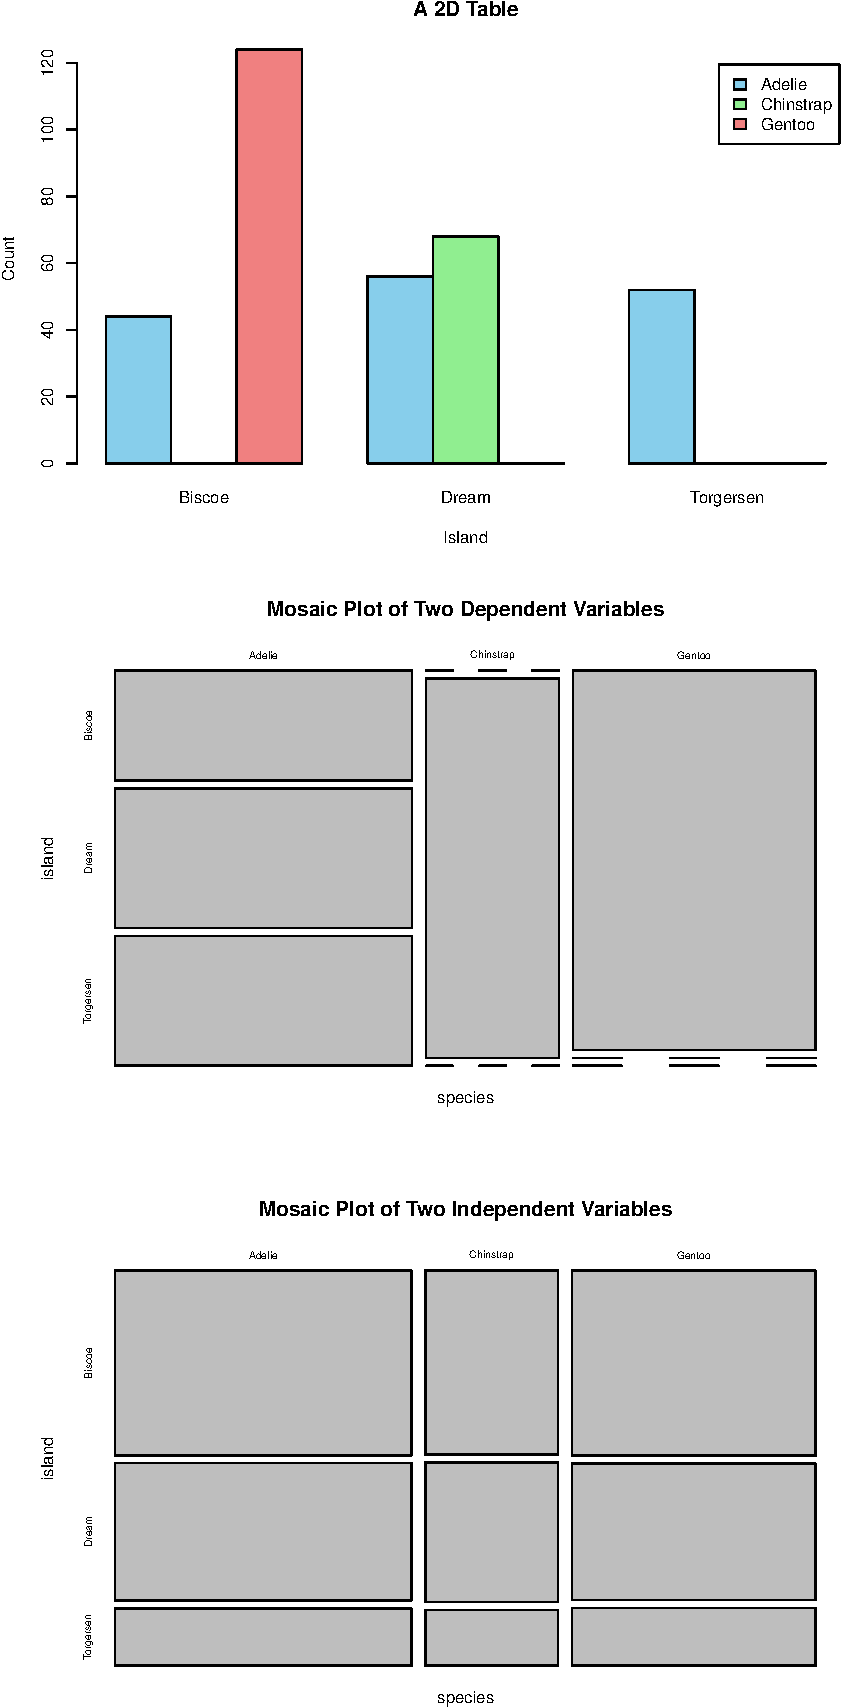
\includegraphics[keepaspectratio]{03_Data_Visualization_files/figure-pdf/fig-3-16-1.pdf}}

}

\caption{\label{fig-3-16}Visualization of a 2D Contingency Table. Top. A
side-by-side barplot. Middle. Mosaic plot. Bottom. Mosaic plot for
independent categorical variables}

\end{figure}%

\subsection{Two Numeric Variables}\label{two-numeric-variables}

A scatter plot is the default choice to visualize the relationship
between two numeric variables. The relationship can be manifold, ranging
from linear to cyclical. So, visualizing how the data points are
distributed in a 2D plan is an intuitive way to learn about there
relationship. Importantly, visualization should be done before
performing any statistical analysis, e.g., linear regression. Here is
how to create a scatter plot that shows the relationship between sepal
width and sepal length. Note that each point \((x_{i},y_{i})\) is a pair
of values from one sample.

\begin{Shaded}
\begin{Highlighting}[]
\FunctionTok{par}\NormalTok{(}\AttributeTok{mfrow=}\FunctionTok{c}\NormalTok{(}\DecValTok{1}\NormalTok{,}\DecValTok{2}\NormalTok{))}

\CommentTok{\# Top left}
\FunctionTok{plot}\NormalTok{(}\AttributeTok{x=}\NormalTok{iris}\SpecialCharTok{$}\NormalTok{Sepal.Width,}
     \AttributeTok{y=}\NormalTok{iris}\SpecialCharTok{$}\NormalTok{Sepal.Length,}
     \AttributeTok{xlab =} \StringTok{"Sepal Width"}\NormalTok{,}
     \AttributeTok{ylab =} \StringTok{"Sepal Length"}\NormalTok{,}
     \AttributeTok{main =} \StringTok{"Default"}\NormalTok{)}

\CommentTok{\# Top right}
\FunctionTok{plot}\NormalTok{(}\AttributeTok{x=}\NormalTok{iris}\SpecialCharTok{$}\NormalTok{Sepal.Width,}
     \AttributeTok{y=}\NormalTok{iris}\SpecialCharTok{$}\NormalTok{Sepal.Length,}
     \AttributeTok{pch=}\DecValTok{3}\NormalTok{,}
     \AttributeTok{xlab =} \StringTok{"Sepal Width"}\NormalTok{,}
     \AttributeTok{ylab =} \StringTok{"Sepal Length"}\NormalTok{,}
     \AttributeTok{main =} \StringTok{"Change the Point Style"}\NormalTok{)}
\end{Highlighting}
\end{Shaded}

\begin{figure}[H]

\centering{

\pandocbounded{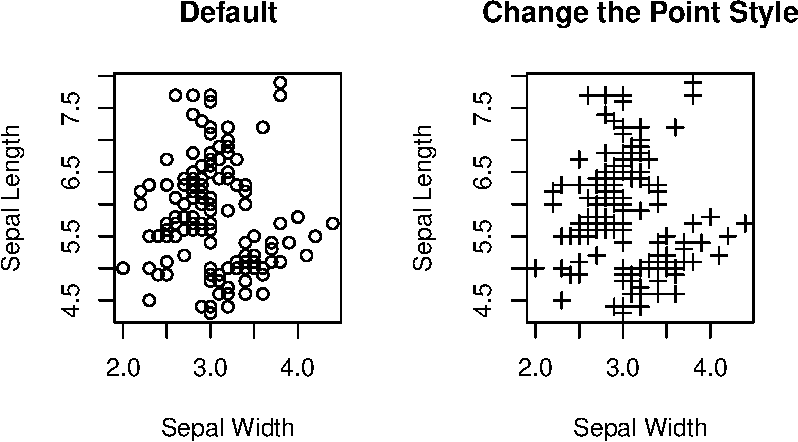
\includegraphics[keepaspectratio]{03_Data_Visualization_files/figure-pdf/fig-3-17-1.pdf}}

}

\caption{\label{fig-3-17}Visualizing the relationship between two
numeric variables.}

\end{figure}%

\begin{Shaded}
\begin{Highlighting}[]
\FunctionTok{plot}\NormalTok{(}\AttributeTok{x=}\NormalTok{iris}\SpecialCharTok{$}\NormalTok{Sepal.Width,}
     \AttributeTok{y=}\NormalTok{iris}\SpecialCharTok{$}\NormalTok{Sepal.Length,}
     \AttributeTok{pch=}\DecValTok{3}\NormalTok{,}
     \AttributeTok{xlab =} \StringTok{"Sepal Width"}\NormalTok{,}
     \AttributeTok{ylab =} \StringTok{"Sepal Length"}\NormalTok{,}
     \AttributeTok{main =} \StringTok{"Segregate Data Points by Color (Species)"}\NormalTok{,}
     \AttributeTok{col =} \FunctionTok{c}\NormalTok{(}\StringTok{"skyblue"}\NormalTok{, }\StringTok{"lightgreen"}\NormalTok{, }\StringTok{"lightcoral"}\NormalTok{)[}\FunctionTok{as.numeric}\NormalTok{(iris}\SpecialCharTok{$}\NormalTok{Species)])}

\FunctionTok{legend}\NormalTok{(}\StringTok{"topright"}\NormalTok{,}
       \AttributeTok{legend =} \FunctionTok{levels}\NormalTok{(iris}\SpecialCharTok{$}\NormalTok{Species),}
       \AttributeTok{col =} \FunctionTok{c}\NormalTok{(}\StringTok{"skyblue"}\NormalTok{, }\StringTok{"lightgreen"}\NormalTok{, }\StringTok{"lightcoral"}\NormalTok{),}
       \AttributeTok{pch =} \DecValTok{3}\NormalTok{,}
       \AttributeTok{title =} \StringTok{"Species"}\NormalTok{)}
\end{Highlighting}
\end{Shaded}

\begin{figure}[H]

\centering{

\pandocbounded{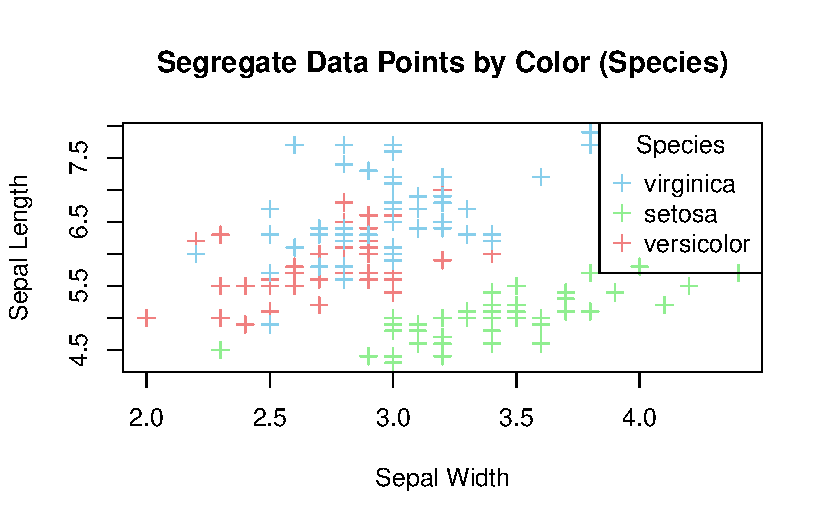
\includegraphics[keepaspectratio]{03_Data_Visualization_files/figure-pdf/fig-3-18-1.pdf}}

}

\caption{\label{fig-3-18}Color data points by species.}

\end{figure}%

If your aim is to explore linear relationship between the two variables,
it can be emphasized by addingg a regression line for the two variables
on top of the data points. Here is an example, regress
\texttt{Sepal.Length} (response) on \texttt{Sepal.Width} (independent).

\begin{Shaded}
\begin{Highlighting}[]
\NormalTok{lm\_model }\OtherTok{\textless{}{-}} \FunctionTok{lm}\NormalTok{(Sepal.Length }\SpecialCharTok{\textasciitilde{}}\NormalTok{ Sepal.Width, }\AttributeTok{data=}\NormalTok{iris)}

\CommentTok{\# intercept}
\NormalTok{intercept }\OtherTok{\textless{}{-}}\NormalTok{ lm\_model}\SpecialCharTok{$}\NormalTok{coefficients[}\DecValTok{1}\NormalTok{]}

\CommentTok{\# slope}
\NormalTok{slope }\OtherTok{=}\NormalTok{ lm\_model}\SpecialCharTok{$}\NormalTok{coefficients[}\DecValTok{2}\NormalTok{]}

\FunctionTok{print}\NormalTok{(}\FunctionTok{paste}\NormalTok{(}\StringTok{"Slope ="}\NormalTok{, slope, }\StringTok{"Intercept ="}\NormalTok{, intercept))}
\end{Highlighting}
\end{Shaded}

\begin{verbatim}
[1] "Slope = -0.2233610611299 Intercept = 6.52622255089448"
\end{verbatim}

\begin{Shaded}
\begin{Highlighting}[]
\FunctionTok{plot}\NormalTok{(}\AttributeTok{x=}\NormalTok{iris}\SpecialCharTok{$}\NormalTok{Sepal.Width,}
     \AttributeTok{y=}\NormalTok{iris}\SpecialCharTok{$}\NormalTok{Sepal.Length,}
     \AttributeTok{pch=}\DecValTok{3}\NormalTok{,}
     \AttributeTok{xlab =} \StringTok{"Sepal Width"}\NormalTok{,}
     \AttributeTok{ylab =} \StringTok{"Sepal Length"}\NormalTok{,}
     \AttributeTok{main =} \StringTok{"Add a Regression Line"}\NormalTok{,}
     \AttributeTok{col =} \FunctionTok{c}\NormalTok{(}\StringTok{"skyblue"}\NormalTok{, }\StringTok{"lightgreen"}\NormalTok{, }\StringTok{"lightcoral"}\NormalTok{)[}\FunctionTok{as.numeric}\NormalTok{(iris}\SpecialCharTok{$}\NormalTok{Species)])}

\FunctionTok{legend}\NormalTok{(}\StringTok{"topright"}\NormalTok{,}
       \AttributeTok{legend =} \FunctionTok{levels}\NormalTok{(iris}\SpecialCharTok{$}\NormalTok{Species),}
       \AttributeTok{col =} \FunctionTok{c}\NormalTok{(}\StringTok{"skyblue"}\NormalTok{, }\StringTok{"lightgreen"}\NormalTok{, }\StringTok{"lightcoral"}\NormalTok{),}
       \AttributeTok{pch =} \DecValTok{3}\NormalTok{,}
       \AttributeTok{title =} \StringTok{"Species"}\NormalTok{)}

\CommentTok{\# Add a line}
\FunctionTok{abline}\NormalTok{(}\AttributeTok{a=}\NormalTok{intercept, }\AttributeTok{b=}\NormalTok{slope, }\AttributeTok{col=}\StringTok{\textquotesingle{}red\textquotesingle{}}\NormalTok{)}
\end{Highlighting}
\end{Shaded}

\begin{figure}[H]

\centering{

\pandocbounded{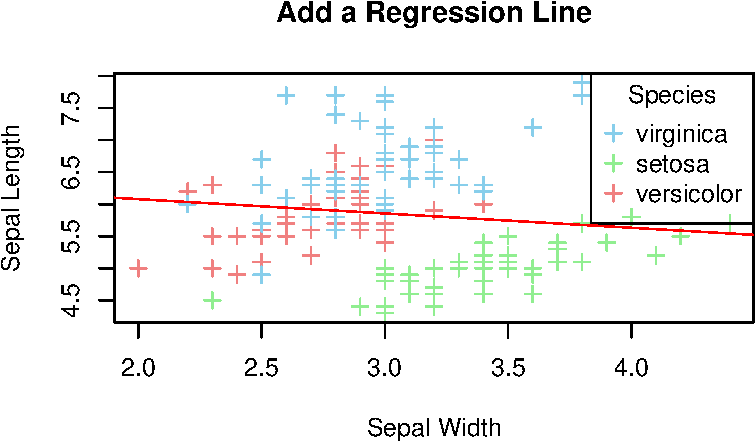
\includegraphics[keepaspectratio]{03_Data_Visualization_files/figure-pdf/fig-3-19-1.pdf}}

}

\caption{\label{fig-3-19}A scatter plot with a regression line.}

\end{figure}%

\subsection{Multipanel Scatter Plot}\label{multipanel-scatter-plot}

A multipanel scatter plot offers a glimpse of the relationship between
all possible pairs of numeric variables. Suppose, you are interested in
the pairwise relationship between all numeric variables in
\texttt{iris}. It can easily be done using the \texttt{pairs()} plot
function.

\begin{Shaded}
\begin{Highlighting}[]
\FunctionTok{pairs}\NormalTok{(iris[,}\DecValTok{1}\SpecialCharTok{:}\DecValTok{4}\NormalTok{], }\AttributeTok{main=}\StringTok{"A Multi{-}Panel Scatter Plot"}\NormalTok{)}
\end{Highlighting}
\end{Shaded}

\begin{figure}[H]

\centering{

\pandocbounded{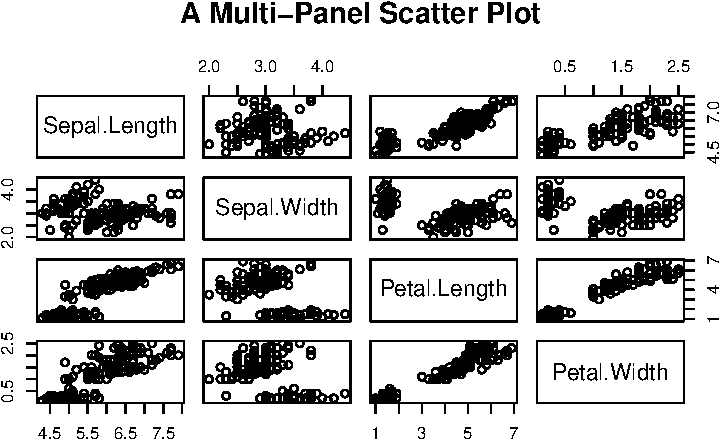
\includegraphics[keepaspectratio]{03_Data_Visualization_files/figure-pdf/fig-3-20-1.pdf}}

}

\caption{\label{fig-3-20}A Multipanel Scatter Plot}

\end{figure}%

Here it concludes our journey of data visualization using base R
functions. As you can see, some plots can be made easily using base R
(e.g., multipanel scatter plot), while others are less direct (e.g., bar
plot with error bars). There is no one system you should use, choose
whatever fits your requirements.

\section{\texorpdfstring{\texttt{ggplot2}}{ggplot2}}\label{ggplot2}

\texttt{ggplot2} is bundled in \texttt{tidyverse}. Once you have
activated \texttt{tidyverse}, \texttt{ggplot2} is available. Here, the
focus is on using \texttt{ggplot2} to plot the graphs that were created
using base R above. We will not repeat the discussion of strengths and
weaknesses of each graph in this section. Readers should refer to the
corresponding section above for the characteristics and functions of the
graphs.

If \texttt{tidyverse} has not been activated, load it into R before
using \texttt{ggplot2}.

\begin{Shaded}
\begin{Highlighting}[]
\FunctionTok{require}\NormalTok{(tidyverse)}
\end{Highlighting}
\end{Shaded}

\begin{verbatim}
Loading required package: tidyverse
\end{verbatim}

\begin{verbatim}
-- Attaching core tidyverse packages ------------------------ tidyverse 2.0.0 --
v dplyr     1.2.1     v readr     2.2.0
v forcats   1.0.1     v stringr   1.6.0
v ggplot2   4.0.3     v tibble    3.3.1
v lubridate 1.9.5     v tidyr     1.3.2
v purrr     1.2.2     
-- Conflicts ------------------------------------------ tidyverse_conflicts() --
x dplyr::filter() masks stats::filter()
x dplyr::lag()    masks stats::lag()
i Use the conflicted package (<http://conflicted.r-lib.org/>) to force all conflicts to become errors
\end{verbatim}

\subsection{\texorpdfstring{Grammar of
\texttt{ggplot2}}{Grammar of ggplot2}}\label{grammar-of-ggplot2}

The two '\texttt{g}'s of \texttt{ggplot2} stand for \textbf{Grammar of
Graphics}. In \texttt{ggplot2}, the graphical widgets are arranged in
layers. That idea gives developers the flexibility to decorate a graph
by adding layers to an existing graph. The \textbf{data} layer forms the
foundation of a graph. The \textbf{Aesthetics} defines the association
between data variable(s) and the axes. \textbf{Geometries} are the types
of graphs, e.g., line plot, histogram, etc. \textbf{Facets} split a
graph into multi-panels. \textbf{Statistics} defines how to aggregate
data, e.g., in proportion or take the face value in a barplot.
\textbf{Coordinates} supports an X-Y Cartesian coordinate system, and a
polar coordinate system. (See the Pie Chart section below)
\textbf{Themes} offers different color schemes, font type, font size,
etc.

\begin{figure}

\centering{

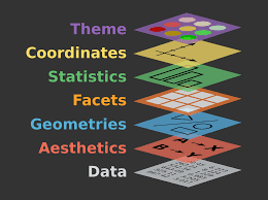
\includegraphics[width=0.5\linewidth,height=0.5\textheight]{images/Figure_3-21-ggplot-anatomy.png}

}

\caption{\label{fig-3-21}Anatomy of \texttt{ggplot2}}

\end{figure}%

\subsection{One Numeric Variable}\label{one-numeric-variable-1}

You can plot a histogram of the numeric variable to see its
distribution, such as the spread, the peak, symmetry, and flatness. If
your concern is robust statistics, make a box plot instead.

\subsubsection{Histogram}\label{histogram-1}

Let's redraw the histogram in Figure~\ref{fig-3-1} using
\texttt{ggplot2}. The first line is the \emph{data layer} that specifies
the data source, and it must be a data frame (or tibble), e.g.,
\texttt{iris}. The \emph{aesthetic} option designates the x-axis for
\texttt{Sepal.Width}. The second line is the \emph{geometry} of the
graph. For a histogram, the function name is \texttt{geom\_histogram()}.
Here is the bare minimum of a \texttt{ggplot2} histogram:

\begin{Shaded}
\begin{Highlighting}[]
\CommentTok{\# Default}
\FunctionTok{ggplot}\NormalTok{(}\AttributeTok{data=}\NormalTok{iris, }\FunctionTok{aes}\NormalTok{(}\AttributeTok{x=}\NormalTok{Sepal.Width)) }\SpecialCharTok{+}
  \FunctionTok{geom\_histogram}\NormalTok{()}
\end{Highlighting}
\end{Shaded}

\begin{verbatim}
`stat_bin()` using `bins = 30`. Pick better value `binwidth`.
\end{verbatim}

\begin{figure}[H]

\centering{

\pandocbounded{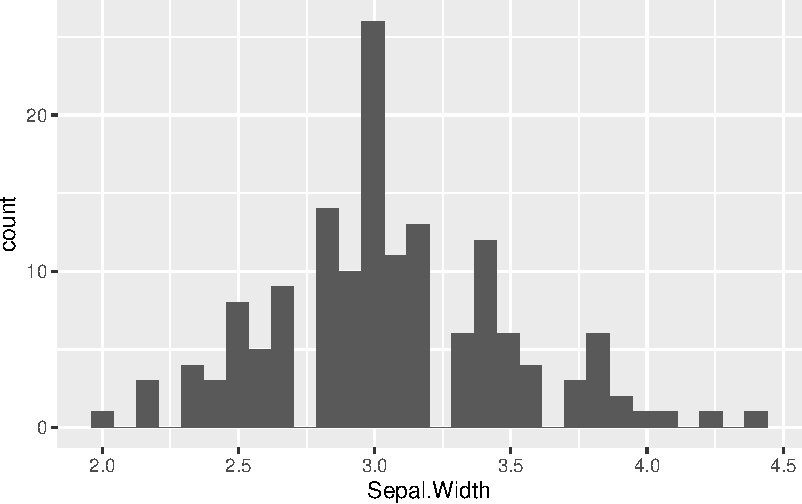
\includegraphics[keepaspectratio]{03_Data_Visualization_files/figure-pdf/fig-3-22-1.pdf}}

}

\caption{\label{fig-3-22}\texttt{ggplot2} Histogram.}

\end{figure}%

\emph{If you see this message: ``\texttt{stat\_bin()} using
\texttt{bins\ =\ 30}. Pick better value \texttt{binwidth}'', R just
informs you that 30 bins was used by default. You can ignore it or
specify a new \texttt{binwidth} value.}

It is always a good idea to give the graph a title at the top so people
know what the key message is. Equally important is the x- and y-labels.
This task can be done by the \texttt{labs()} function. By default, the
title is left-justified. To center it, see the last line and the comment
above it.

\begin{Shaded}
\begin{Highlighting}[]
\CommentTok{\# Overwrite default x{-}/y{-}label and title}
\FunctionTok{ggplot}\NormalTok{(}\AttributeTok{data=}\NormalTok{iris, }\FunctionTok{aes}\NormalTok{(}\AttributeTok{x=}\NormalTok{Sepal.Width)) }\SpecialCharTok{+}
  \FunctionTok{geom\_histogram}\NormalTok{() }\SpecialCharTok{+}
  \FunctionTok{labs}\NormalTok{(}\AttributeTok{x=}\StringTok{"Sepal Width"}\NormalTok{, }\AttributeTok{y=}\StringTok{"Count"}\NormalTok{, }\AttributeTok{title=}\StringTok{"Histogram of Sepal Width"}\NormalTok{) }\SpecialCharTok{+}
  \CommentTok{\# hjust = 0.5 means the horizontal adjustment is the midpoint.}
  \FunctionTok{theme}\NormalTok{(}\AttributeTok{plot.title =} \FunctionTok{element\_text}\NormalTok{(}\AttributeTok{hjust =} \FloatTok{0.5}\NormalTok{))}
\end{Highlighting}
\end{Shaded}

\begin{verbatim}
`stat_bin()` using `bins = 30`. Pick better value `binwidth`.
\end{verbatim}

\begin{figure}[H]

\centering{

\pandocbounded{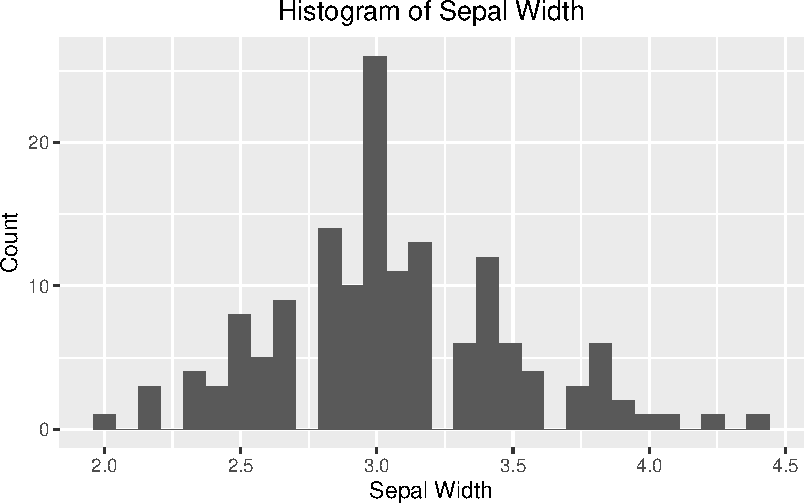
\includegraphics[keepaspectratio]{03_Data_Visualization_files/figure-pdf/fig-3-23-1.pdf}}

}

\caption{\label{fig-3-23}A \texttt{ggplot2} Histogram with customized
labels and title.}

\end{figure}%

Change the fill color and border color. It can be done by providing
additional parameters to the \texttt{geom\_histogram()}.

\begin{Shaded}
\begin{Highlighting}[]
\CommentTok{\# fill = filled color}
\CommentTok{\# color = border color}
\FunctionTok{ggplot}\NormalTok{(}\AttributeTok{data=}\NormalTok{iris, }\FunctionTok{aes}\NormalTok{(}\AttributeTok{x=}\NormalTok{Sepal.Width)) }\SpecialCharTok{+}
  \FunctionTok{geom\_histogram}\NormalTok{(}\AttributeTok{fill=}\StringTok{"skyblue"}\NormalTok{, }\AttributeTok{color =} \StringTok{"white"}\NormalTok{) }\SpecialCharTok{+}
  \FunctionTok{labs}\NormalTok{(}\AttributeTok{x=}\StringTok{"Sepal Width"}\NormalTok{, }\AttributeTok{y=}\StringTok{"Count"}\NormalTok{, }\AttributeTok{title=}\StringTok{"Color Options"}\NormalTok{) }\SpecialCharTok{+}
  \CommentTok{\# hjust = 0.5 means the horizontal adjustment is the midpoint.}
  \FunctionTok{theme}\NormalTok{(}\AttributeTok{plot.title =} \FunctionTok{element\_text}\NormalTok{(}\AttributeTok{hjust =} \FloatTok{0.5}\NormalTok{))}
\end{Highlighting}
\end{Shaded}

\begin{verbatim}
`stat_bin()` using `bins = 30`. Pick better value `binwidth`.
\end{verbatim}

\begin{figure}[H]

\centering{

\pandocbounded{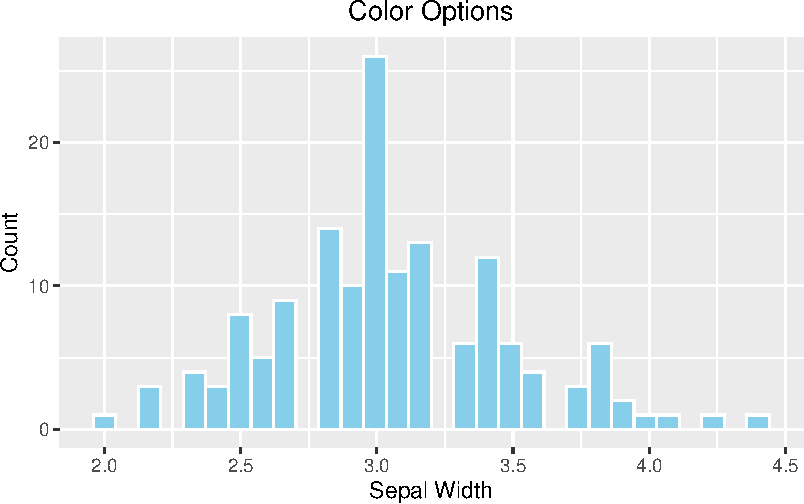
\includegraphics[keepaspectratio]{03_Data_Visualization_files/figure-pdf/fig-3-24-1.pdf}}

}

\caption{\label{fig-3-24}A \texttt{ggplot2} Histogram with a customized
color.}

\end{figure}%

The bin width of a histogram is calculated automatically by
\texttt{ggplot2} according to the range of x. You can use the
\texttt{breaks} parameter to overwrite it.

\begin{Shaded}
\begin{Highlighting}[]
\CommentTok{\# breaks}
\FunctionTok{ggplot}\NormalTok{(}\AttributeTok{data=}\NormalTok{iris, }\FunctionTok{aes}\NormalTok{(}\AttributeTok{x=}\NormalTok{Sepal.Width)) }\SpecialCharTok{+}
  \FunctionTok{geom\_histogram}\NormalTok{(}\AttributeTok{fill=}\StringTok{"skyblue"}\NormalTok{, }\AttributeTok{color =} \StringTok{"white"}\NormalTok{, }\AttributeTok{breaks=}\FunctionTok{seq}\NormalTok{(}\DecValTok{2}\NormalTok{,}\FloatTok{4.5}\NormalTok{,}\AttributeTok{by=}\FloatTok{0.1}\NormalTok{)) }\SpecialCharTok{+}
  \FunctionTok{labs}\NormalTok{(}\AttributeTok{x=}\StringTok{"Sepal Width"}\NormalTok{, }\AttributeTok{y=}\StringTok{"Count"}\NormalTok{, }\AttributeTok{title=}\StringTok{"\textasciigrave{}breaks\textasciigrave{} option"}\NormalTok{) }\SpecialCharTok{+}
  \CommentTok{\# hjust = 0.5 means the horizontal adjustment is the midpoint.}
  \FunctionTok{theme}\NormalTok{(}\AttributeTok{plot.title =} \FunctionTok{element\_text}\NormalTok{(}\AttributeTok{hjust =} \FloatTok{0.5}\NormalTok{))}
\end{Highlighting}
\end{Shaded}

\begin{figure}[H]

\centering{

\pandocbounded{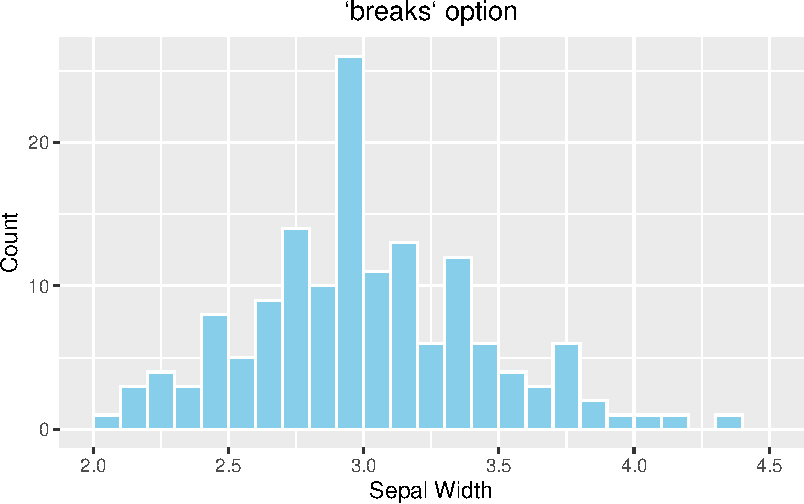
\includegraphics[keepaspectratio]{03_Data_Visualization_files/figure-pdf/fig-3-25-1.pdf}}

}

\caption{\label{fig-3-25}A \texttt{ggplot2} Histogram with a non-default
bin width.}

\end{figure}%

\textbf{Optional topic}

As you might notice that each of the four histograms occupies the entire
plotting area instead of displaying in a 2x2 grid as
Figure~\ref{fig-3-1}. It is because \texttt{ggolot2} does not work with
\texttt{par(mfrow(2,2))}. To divide the plotting area into a grid that
is compatible with \texttt{ggplot2}, use the \texttt{patchwork} package.
Use the menu option \textbf{Tools} \(\rightarrow\) Install Packages to
install it.

Another new concept is that a graph can be stored in a variable so it
can be displayed later in the grid. In the example below, the four
histograms above are initially stored in variables \texttt{p1},
\texttt{p2}, \texttt{p3}, and \texttt{p4}. See the example below:

\begin{Shaded}
\begin{Highlighting}[]
\FunctionTok{require}\NormalTok{(patchwork)}

\CommentTok{\# Default}
\NormalTok{p1 }\OtherTok{\textless{}{-}} \FunctionTok{ggplot}\NormalTok{(}\AttributeTok{data=}\NormalTok{iris, }\FunctionTok{aes}\NormalTok{(}\AttributeTok{x=}\NormalTok{Sepal.Width)) }\SpecialCharTok{+}
        \FunctionTok{geom\_histogram}\NormalTok{()}

\CommentTok{\# With labels and title}
\NormalTok{p2 }\OtherTok{\textless{}{-}} \FunctionTok{ggplot}\NormalTok{(}\AttributeTok{data=}\NormalTok{iris, }\FunctionTok{aes}\NormalTok{(}\AttributeTok{x=}\NormalTok{Sepal.Width)) }\SpecialCharTok{+}
        \FunctionTok{geom\_histogram}\NormalTok{() }\SpecialCharTok{+}
        \FunctionTok{labs}\NormalTok{(}\AttributeTok{x=}\StringTok{"Sepal Width"}\NormalTok{, }\AttributeTok{y=}\StringTok{"Count"}\NormalTok{, }\AttributeTok{title=}\StringTok{"Histogram of Sepal Width"}\NormalTok{) }\SpecialCharTok{+}
        \CommentTok{\# hjust = 0.5 means the horizontal adjustment is the midpoint.}
        \FunctionTok{theme}\NormalTok{(}\AttributeTok{plot.title =} \FunctionTok{element\_text}\NormalTok{(}\AttributeTok{hjust =} \FloatTok{0.5}\NormalTok{))}

\CommentTok{\# fill = filled color}
\CommentTok{\# colour = border color}
\NormalTok{p3 }\OtherTok{\textless{}{-}} \FunctionTok{ggplot}\NormalTok{(}\AttributeTok{data=}\NormalTok{iris, }\FunctionTok{aes}\NormalTok{(}\AttributeTok{x=}\NormalTok{Sepal.Width)) }\SpecialCharTok{+}
        \FunctionTok{geom\_histogram}\NormalTok{(}\AttributeTok{fill=}\StringTok{"skyblue"}\NormalTok{, }\AttributeTok{color =} \StringTok{"white"}\NormalTok{) }\SpecialCharTok{+}
        \FunctionTok{labs}\NormalTok{(}\AttributeTok{x=}\StringTok{"Sepal Width"}\NormalTok{, }\AttributeTok{y=}\StringTok{"Count"}\NormalTok{, }\AttributeTok{title=}\StringTok{"Color Options"}\NormalTok{) }\SpecialCharTok{+}
        \CommentTok{\# hjust = 0.5 means the horizontal adjustment is the midpoint.}
        \FunctionTok{theme}\NormalTok{(}\AttributeTok{plot.title =} \FunctionTok{element\_text}\NormalTok{(}\AttributeTok{hjust =} \FloatTok{0.5}\NormalTok{))}

\CommentTok{\# Change the number of bins}
\NormalTok{p4 }\OtherTok{\textless{}{-}} \FunctionTok{ggplot}\NormalTok{(}\AttributeTok{data=}\NormalTok{iris, }\FunctionTok{aes}\NormalTok{(}\AttributeTok{x=}\NormalTok{Sepal.Width)) }\SpecialCharTok{+}
        \FunctionTok{geom\_histogram}\NormalTok{(}\AttributeTok{fill=}\StringTok{"skyblue"}\NormalTok{, }\AttributeTok{color =} \StringTok{"white"}\NormalTok{, }\AttributeTok{breaks=}\FunctionTok{seq}\NormalTok{(}\DecValTok{2}\NormalTok{,}\FloatTok{4.5}\NormalTok{,}\AttributeTok{by=}\FloatTok{0.1}\NormalTok{)) }\SpecialCharTok{+}
        \FunctionTok{labs}\NormalTok{(}\AttributeTok{x=}\StringTok{"Sepal Width"}\NormalTok{, }\AttributeTok{y=}\StringTok{"Count"}\NormalTok{, }\AttributeTok{title=}\StringTok{"\textasciigrave{}breaks\textasciigrave{} option"}\NormalTok{) }\SpecialCharTok{+}
        \CommentTok{\# hjust = 0.5 means the horizontal adjustment is the midpoint.}
        \FunctionTok{theme}\NormalTok{(}\AttributeTok{plot.title =} \FunctionTok{element\_text}\NormalTok{(}\AttributeTok{hjust =} \FloatTok{0.5}\NormalTok{))}

\CommentTok{\# Arrange them in a 2x2 grid}
\CommentTok{\# \textquotesingle{}+\textquotesingle{} places plots next to each other, \textquotesingle{}/\textquotesingle{} stacks them}
\NormalTok{(p1 }\SpecialCharTok{+}\NormalTok{ p2) }\SpecialCharTok{/}\NormalTok{ (p3 }\SpecialCharTok{+}\NormalTok{ p4)}
\end{Highlighting}
\end{Shaded}

\begin{figure}[H]

\centering{

\pandocbounded{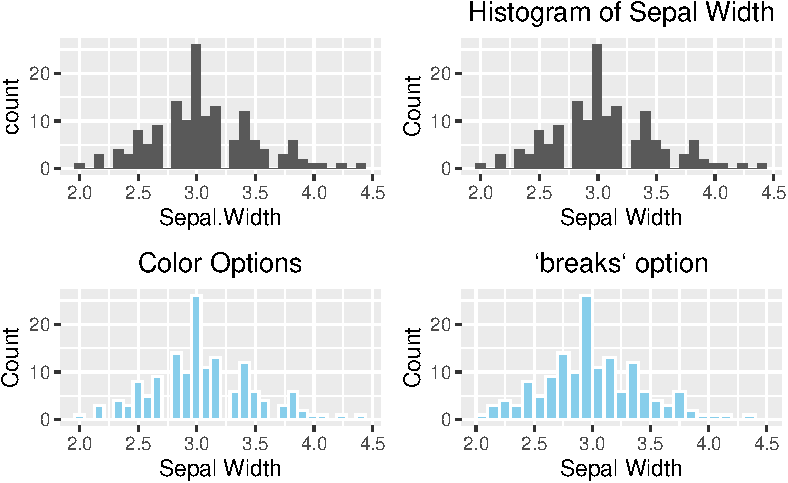
\includegraphics[keepaspectratio]{03_Data_Visualization_files/figure-pdf/fig-3-26-1.pdf}}

}

\caption{\label{fig-3-26}\texttt{ggplot2} Grid System by
\texttt{patchwork}. Top left: Default (bare minimum). Top right: with
labels and title. Bottom left: change the color. Bottom right: change
the number of bins.}

\end{figure}%

\subsubsection{Box plot}\label{box-plot-1}

The anatomy of a box plot can be found in Figure~\ref{fig-3-3}. The
geometry function of a box plot is \texttt{geom\_boxplot()}. Unlike a
histogram, the numeric variable is mapped to the y-axis for a vertical
box plot. If you want a horizontal box plot, map the numeric variable to
the x-axis, and don't forget to specify the label for the x-axis.

\begin{Shaded}
\begin{Highlighting}[]
\FunctionTok{require}\NormalTok{(patchwork)}

\CommentTok{\# Default}
\NormalTok{p1 }\OtherTok{\textless{}{-}} \FunctionTok{ggplot}\NormalTok{(}\AttributeTok{data=}\NormalTok{iris, }\FunctionTok{aes}\NormalTok{(}\AttributeTok{y=}\NormalTok{Sepal.Width)) }\SpecialCharTok{+}
        \FunctionTok{geom\_boxplot}\NormalTok{()}

\CommentTok{\# Add y{-}label and title}
\NormalTok{p2 }\OtherTok{\textless{}{-}} \FunctionTok{ggplot}\NormalTok{(}\AttributeTok{data=}\NormalTok{iris, }\FunctionTok{aes}\NormalTok{(}\AttributeTok{y=}\NormalTok{Sepal.Width)) }\SpecialCharTok{+}
        \FunctionTok{geom\_boxplot}\NormalTok{() }\SpecialCharTok{+}
        \FunctionTok{labs}\NormalTok{(}\AttributeTok{y=}\StringTok{"Sepal Width"}\NormalTok{, }\AttributeTok{title =} \StringTok{"box plot of Sepal Width"}\NormalTok{) }\SpecialCharTok{+}
        \FunctionTok{theme}\NormalTok{(}\AttributeTok{plot.title =} \FunctionTok{element\_text}\NormalTok{(}\AttributeTok{hjust =} \FloatTok{0.5}\NormalTok{))}

\CommentTok{\# Change color}
\NormalTok{p3 }\OtherTok{\textless{}{-}} \FunctionTok{ggplot}\NormalTok{(}\AttributeTok{data=}\NormalTok{iris, }\FunctionTok{aes}\NormalTok{(}\AttributeTok{y=}\NormalTok{Sepal.Width)) }\SpecialCharTok{+}
        \FunctionTok{geom\_boxplot}\NormalTok{(}\AttributeTok{fill=}\StringTok{"skyblue"}\NormalTok{, }\AttributeTok{outlier.color =} \StringTok{"red"}\NormalTok{) }\SpecialCharTok{+}
        \FunctionTok{labs}\NormalTok{(}\AttributeTok{y=}\StringTok{"Sepal Width"}\NormalTok{, }\AttributeTok{title =} \StringTok{"Color options"}\NormalTok{) }\SpecialCharTok{+}
        \FunctionTok{theme}\NormalTok{(}\AttributeTok{plot.title =} \FunctionTok{element\_text}\NormalTok{(}\AttributeTok{hjust =} \FloatTok{0.5}\NormalTok{))}

\CommentTok{\# Horizontal box plot}
\NormalTok{p4 }\OtherTok{\textless{}{-}} \FunctionTok{ggplot}\NormalTok{(}\AttributeTok{data=}\NormalTok{iris, }\FunctionTok{aes}\NormalTok{(}\AttributeTok{x=}\NormalTok{Sepal.Width)) }\SpecialCharTok{+}
        \FunctionTok{geom\_boxplot}\NormalTok{() }\SpecialCharTok{+}
        \FunctionTok{labs}\NormalTok{(}\AttributeTok{x=}\StringTok{"Sepal Width"}\NormalTok{, }\AttributeTok{title =} \StringTok{"Horizontal box plot"}\NormalTok{) }\SpecialCharTok{+}
        \FunctionTok{theme}\NormalTok{(}\AttributeTok{plot.title =} \FunctionTok{element\_text}\NormalTok{(}\AttributeTok{hjust =} \FloatTok{0.5}\NormalTok{))}

\NormalTok{(p1 }\SpecialCharTok{+}\NormalTok{ p2)}\SpecialCharTok{/}\NormalTok{(p3 }\SpecialCharTok{+}\NormalTok{ p4)}
\end{Highlighting}
\end{Shaded}

\begin{figure}[H]

\centering{

\pandocbounded{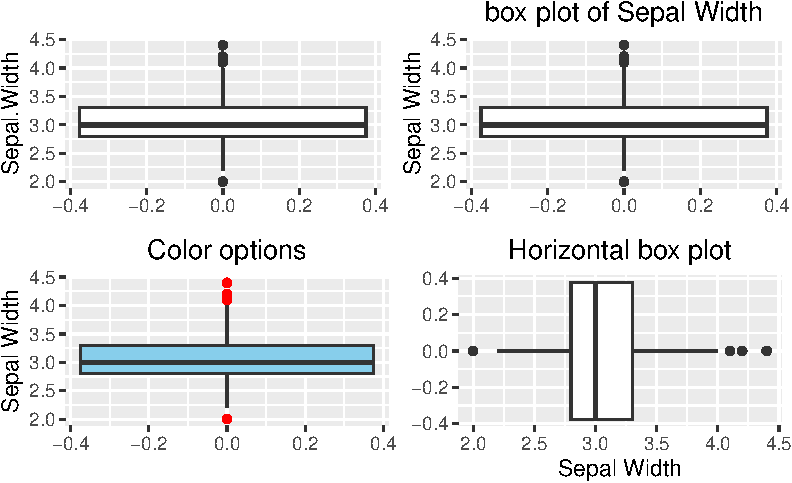
\includegraphics[keepaspectratio]{03_Data_Visualization_files/figure-pdf/fig-3-27-1.pdf}}

}

\caption{\label{fig-3-27}box plot using \texttt{ggplot2}. Top left:
default (bare minimum). Top right: with y-label and title. Bottom left:
change color. Bottom right: horizontal box plot.}

\end{figure}%

\subsection{One Categorical Variable}\label{one-categorical-variable-1}

\subsubsection{Bar Plot}\label{bar-plot-1}

Here we will show how to make a bar plot and a pie chart using
\texttt{ggplot2}.

\begin{Shaded}
\begin{Highlighting}[]
\FunctionTok{require}\NormalTok{(patchwork)}

\CommentTok{\# Default}
\NormalTok{p1 }\OtherTok{\textless{}{-}} \FunctionTok{ggplot}\NormalTok{(}\AttributeTok{data=}\NormalTok{iris, }\FunctionTok{aes}\NormalTok{(}\AttributeTok{x=}\NormalTok{Species)) }\SpecialCharTok{+}
        \FunctionTok{geom\_bar}\NormalTok{()}

\CommentTok{\# With labels and title}
\NormalTok{p2 }\OtherTok{\textless{}{-}} \FunctionTok{ggplot}\NormalTok{(}\AttributeTok{data=}\NormalTok{iris, }\FunctionTok{aes}\NormalTok{(}\AttributeTok{x=}\NormalTok{Species)) }\SpecialCharTok{+}
        \FunctionTok{geom\_bar}\NormalTok{() }\SpecialCharTok{+}
        \FunctionTok{labs}\NormalTok{(}\AttributeTok{x=}\StringTok{"Species"}\NormalTok{, }\AttributeTok{y=}\StringTok{"Count"}\NormalTok{, }\AttributeTok{title =} \StringTok{"A Barplot of Species"}\NormalTok{) }\SpecialCharTok{+}
        \FunctionTok{theme}\NormalTok{(}\AttributeTok{plot.title =} \FunctionTok{element\_text}\NormalTok{(}\AttributeTok{hjust =} \FloatTok{0.5}\NormalTok{))}

\CommentTok{\# Color option}
\NormalTok{p3 }\OtherTok{\textless{}{-}} \FunctionTok{ggplot}\NormalTok{(}\AttributeTok{data=}\NormalTok{iris, }\FunctionTok{aes}\NormalTok{(}\AttributeTok{x=}\NormalTok{Species)) }\SpecialCharTok{+}
        \FunctionTok{geom\_bar}\NormalTok{(}\AttributeTok{fill=}\StringTok{"skyblue"}\NormalTok{, }\AttributeTok{color=}\StringTok{"blue"}\NormalTok{) }\SpecialCharTok{+}
        \FunctionTok{labs}\NormalTok{(}\AttributeTok{x=}\StringTok{"Species"}\NormalTok{, }\AttributeTok{y=}\StringTok{"Count"}\NormalTok{, }\AttributeTok{title =} \StringTok{"A Barplot of Species"}\NormalTok{) }\SpecialCharTok{+}
        \FunctionTok{theme}\NormalTok{(}\AttributeTok{plot.title =} \FunctionTok{element\_text}\NormalTok{(}\AttributeTok{hjust =} \FloatTok{0.5}\NormalTok{))}

\CommentTok{\# Horizontal barplot}
\NormalTok{p4 }\OtherTok{\textless{}{-}} \FunctionTok{ggplot}\NormalTok{(}\AttributeTok{data=}\NormalTok{iris, }\FunctionTok{aes}\NormalTok{(}\AttributeTok{y=}\NormalTok{Species)) }\SpecialCharTok{+}
        \FunctionTok{geom\_bar}\NormalTok{(}\AttributeTok{fill=}\StringTok{"skyblue"}\NormalTok{, }\AttributeTok{color=}\StringTok{"blue"}\NormalTok{) }\SpecialCharTok{+}
        \FunctionTok{labs}\NormalTok{(}\AttributeTok{y=}\StringTok{"Species"}\NormalTok{, }\AttributeTok{x=}\StringTok{"Count"}\NormalTok{, }\AttributeTok{title =} \StringTok{"A Horizontal Barplot of Species"}\NormalTok{) }\SpecialCharTok{+}
        \FunctionTok{theme}\NormalTok{(}\AttributeTok{plot.title =} \FunctionTok{element\_text}\NormalTok{(}\AttributeTok{hjust =} \FloatTok{0.5}\NormalTok{))}

\NormalTok{(p1 }\SpecialCharTok{+}\NormalTok{ p2)}\SpecialCharTok{/}\NormalTok{(p3 }\SpecialCharTok{+}\NormalTok{ p4)}
\end{Highlighting}
\end{Shaded}

\begin{figure}[H]

\centering{

\pandocbounded{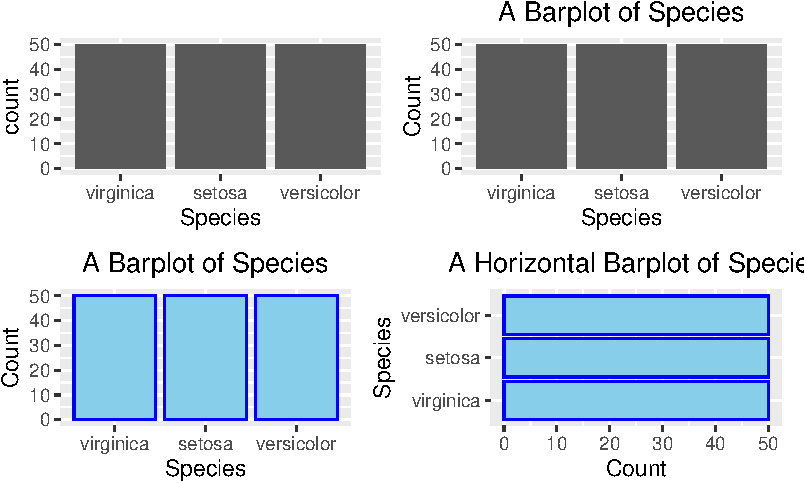
\includegraphics[keepaspectratio]{03_Data_Visualization_files/figure-pdf/fig-3-28-1.pdf}}

}

\caption{\label{fig-3-28}Barplot using \texttt{ggplot2}. Top left:
default (bare minimum).}

\end{figure}%

\subsubsection{Pie Chart}\label{pie-chart-1}

Here's a curve ball. You may give an impression that \texttt{ggplots} is
an upgrade. Plotting a pie chart should be a piece of cake. The fact is
NO.

Despite the the disappointment, it is worth to see how a pie chart can
be plotted using the foundational building-block functions. To give you
a heads-up, \texttt{ggplot2} views a pie chart as a twisted bar plot.
There is an internal logic to justify such a view but we will not
discuss it in detail.

Suppose we want to create a pie chart like the one below:

\begin{figure}

\centering{

\pandocbounded{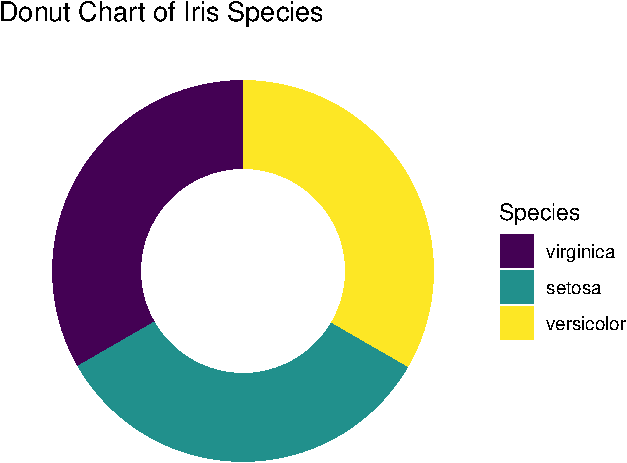
\includegraphics[keepaspectratio]{03_Data_Visualization_files/figure-pdf/fig-3-29-1.pdf}}

}

\caption{\label{fig-3-29}Pie chart or a donut chart}

\end{figure}%

Here we will walk through each of the intermediate steps until getting
the final pie chart.

Let's begin with a stacked barplot, where the bars are stacked up into a
single column, and the fill-color is an attribute to distinguish
different iris species (\texttt{fill=Species}). The stacked bar is
placed at the position 2 units on the right from the origin
(\texttt{aes(x=2)}), but the exact position does not matter.

\begin{Shaded}
\begin{Highlighting}[]
\FunctionTok{ggplot}\NormalTok{(}\AttributeTok{data=}\NormalTok{iris, }\FunctionTok{aes}\NormalTok{(}\AttributeTok{x=}\DecValTok{2}\NormalTok{, }\AttributeTok{fill=}\NormalTok{Species)) }\SpecialCharTok{+}
  \FunctionTok{geom\_bar}\NormalTok{()}
\end{Highlighting}
\end{Shaded}

\begin{figure}[H]

\centering{

\pandocbounded{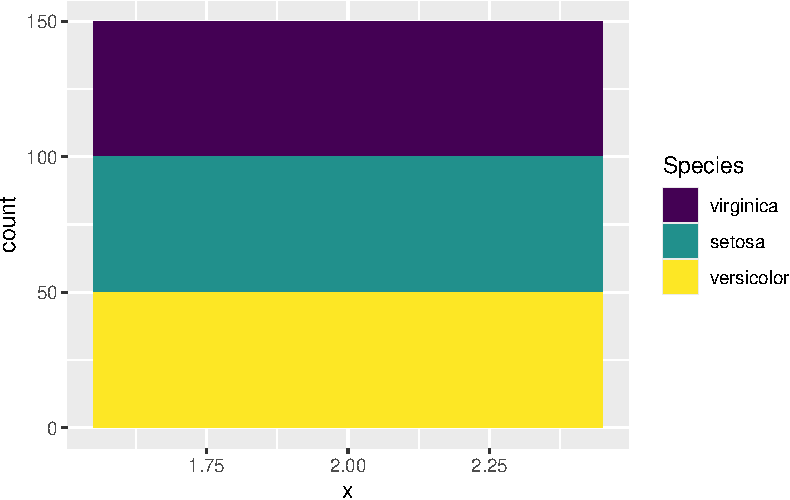
\includegraphics[keepaspectratio]{03_Data_Visualization_files/figure-pdf/fig-3-30-1.pdf}}

}

\caption{\label{fig-3-30}A stacked barplot}

\end{figure}%

Now, use your imagination to picture that the stacked bar is bent into a
ring. Does it look like the pie chart in Figure~\ref{fig-3-30}? To way
to ``bend'' it in \texttt{ggplot2} is to change the x-y Cartesian
coordinate system to the polar (circular) coordinate system in which a
point is characterized by two parameters: the distance from the origin
(\(r\)), and the angle (\(\theta\)) from the horizontal \textbf{polar
axis} in an counter-clockwise direction.

\begin{figure}

\centering{

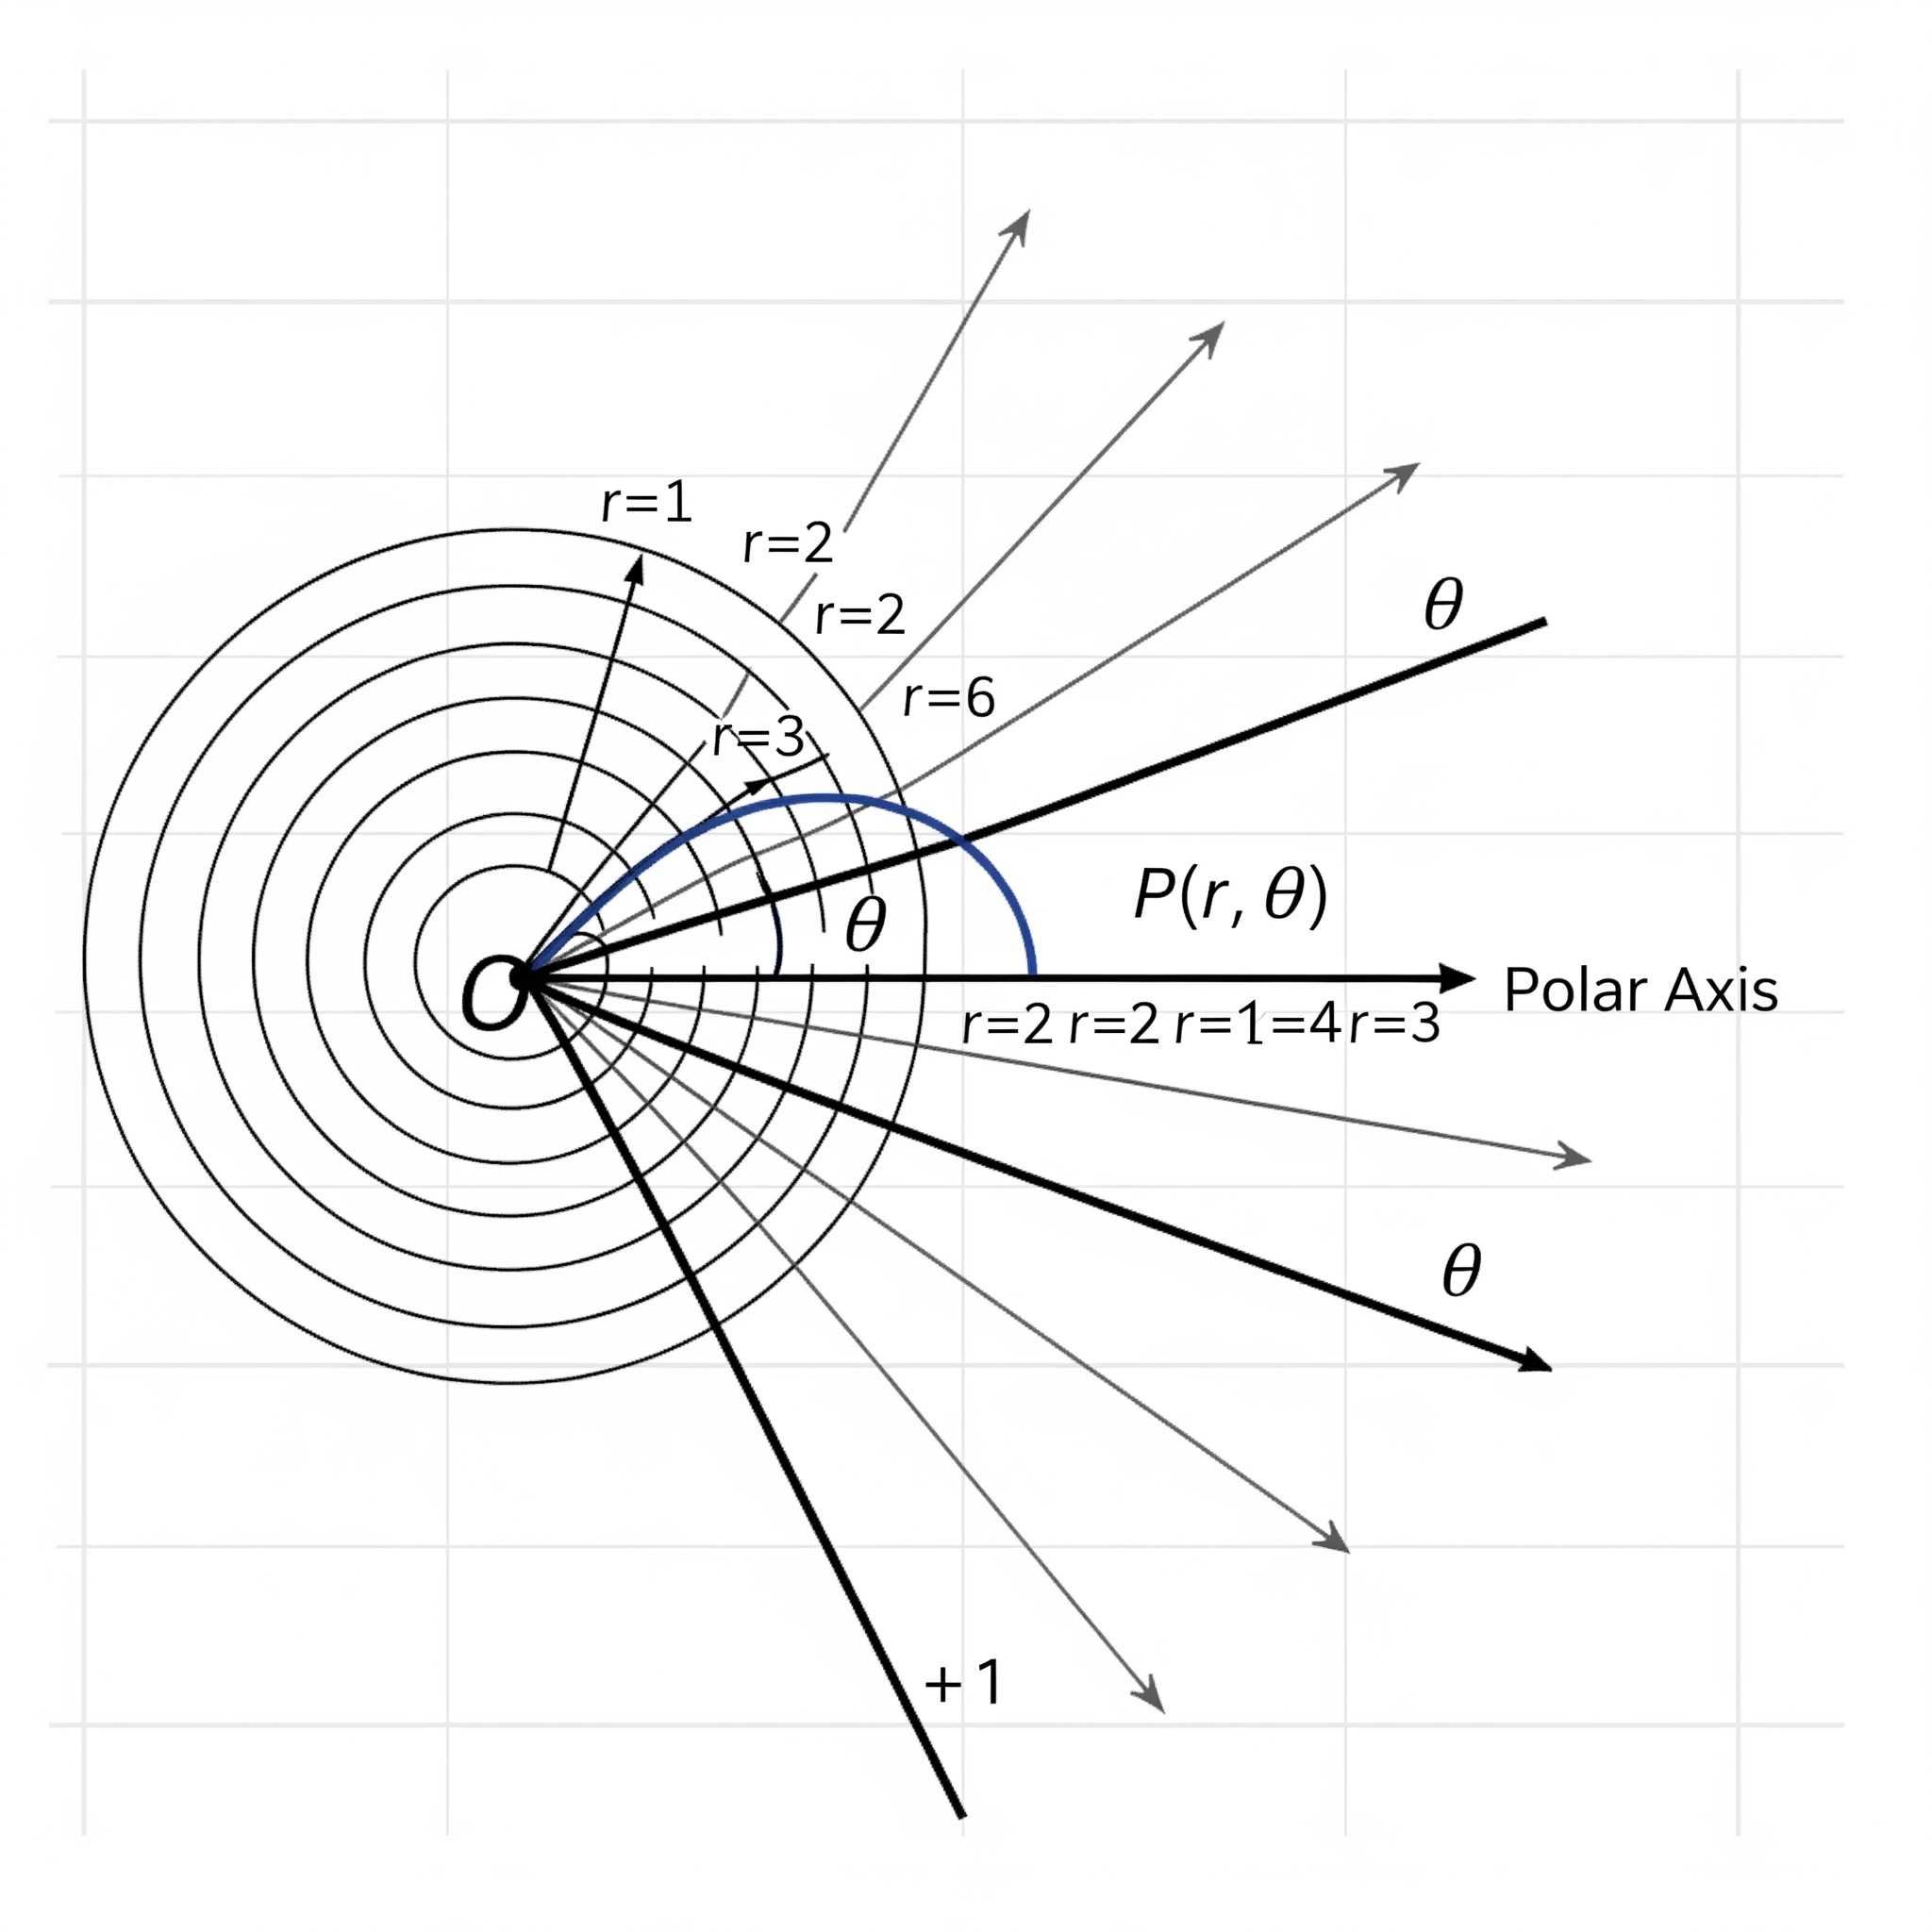
\includegraphics[width=0.5\linewidth,height=0.5\textheight]{images/Figure_3-25-polar-coords.png}

}

\caption{\label{fig-3-31}Polar Coordinate. (generated by Gemini)}

\end{figure}%

By adding this line \texttt{coord\_polar(theta="y",\ start\ =\ 0)} in
the code below, it transforms the height of the bar for each species
into an angle (\(\theta\)) in the polar coordinate, where the zero
position is the 12 o'clock (\texttt{start\ =\ 0}). In this example, one
third of the samples is \texttt{setosa}. As such, the angle \(\theta\)
is \(360^{\circ}\times\frac{1}{3}=120^{\circ}\). If the proportion is a
quarter, the angle \(\theta=360^{\circ}\times\frac{1}{4}=90^{\circ}\).

\begin{Shaded}
\begin{Highlighting}[]
\FunctionTok{ggplot}\NormalTok{(}\AttributeTok{data=}\NormalTok{iris, }\FunctionTok{aes}\NormalTok{(}\AttributeTok{x=}\StringTok{""}\NormalTok{, }\AttributeTok{fill=}\NormalTok{Species)) }\SpecialCharTok{+}
  \FunctionTok{geom\_bar}\NormalTok{() }\SpecialCharTok{+} 
  \FunctionTok{coord\_polar}\NormalTok{(}\AttributeTok{theta=}\StringTok{"y"}\NormalTok{, }\AttributeTok{start =} \DecValTok{0}\NormalTok{)}
\end{Highlighting}
\end{Shaded}

\begin{figure}[H]

\centering{

\pandocbounded{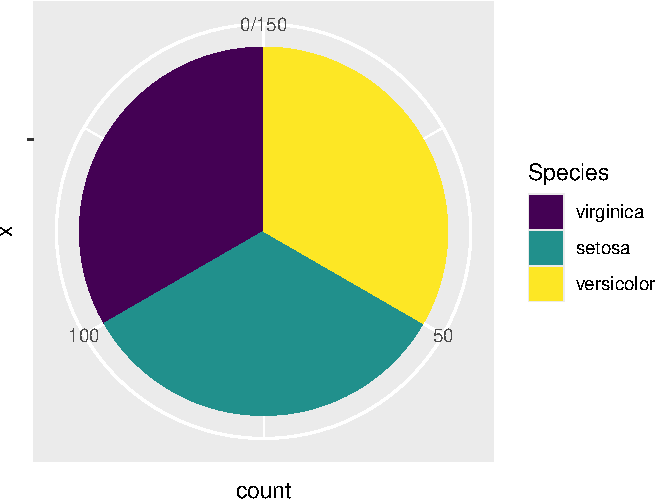
\includegraphics[keepaspectratio]{03_Data_Visualization_files/figure-pdf/fig-3-32-1.pdf}}

}

\caption{\label{fig-3-32}A Piechart by changing to the polar coordinate
system.}

\end{figure}%

The final step is to open a hole in the pie chart if you like, for
aesthetic reasons. But this modification is optional.

\begin{Shaded}
\begin{Highlighting}[]
\FunctionTok{ggplot}\NormalTok{(iris, }\FunctionTok{aes}\NormalTok{(}\AttributeTok{x =} \DecValTok{2}\NormalTok{, }\AttributeTok{fill =}\NormalTok{ Species)) }\SpecialCharTok{+}
  \FunctionTok{geom\_bar}\NormalTok{(}\AttributeTok{width =} \DecValTok{1}\NormalTok{, }\AttributeTok{stat =} \StringTok{"count"}\NormalTok{) }\SpecialCharTok{+}
  \FunctionTok{coord\_polar}\NormalTok{(}\AttributeTok{theta =} \StringTok{"y"}\NormalTok{, }\AttributeTok{start =} \DecValTok{0}\NormalTok{) }\SpecialCharTok{+}
  \CommentTok{\# This is the key part that creates the hole}
  \FunctionTok{xlim}\NormalTok{(}\FloatTok{0.5}\NormalTok{, }\FloatTok{2.5}\NormalTok{) }\SpecialCharTok{+}
  \FunctionTok{labs}\NormalTok{(}\AttributeTok{title =} \StringTok{"Donut Chart of Iris Species"}\NormalTok{)}
\end{Highlighting}
\end{Shaded}

\begin{figure}[H]

\centering{

\pandocbounded{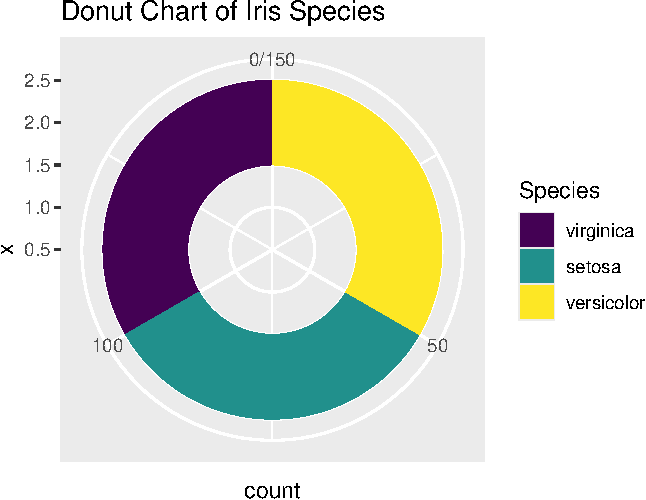
\includegraphics[keepaspectratio]{03_Data_Visualization_files/figure-pdf/fig-3-33-1.pdf}}

}

\caption{\label{fig-3-33}A Piechart using \texttt{ggplot2}.}

\end{figure}%

If you prefer to have a clean background, add the line
\texttt{theme\_void()}. Finally, here's the desired pie chart. What a
journey!

\begin{Shaded}
\begin{Highlighting}[]
\FunctionTok{ggplot}\NormalTok{(iris, }\FunctionTok{aes}\NormalTok{(}\AttributeTok{x =} \DecValTok{2}\NormalTok{, }\AttributeTok{fill =}\NormalTok{ Species)) }\SpecialCharTok{+}
  \FunctionTok{geom\_bar}\NormalTok{(}\AttributeTok{width =} \DecValTok{1}\NormalTok{, }\AttributeTok{stat =} \StringTok{"count"}\NormalTok{) }\SpecialCharTok{+}
  \FunctionTok{coord\_polar}\NormalTok{(}\AttributeTok{theta =} \StringTok{"y"}\NormalTok{, }\AttributeTok{start =} \DecValTok{0}\NormalTok{) }\SpecialCharTok{+}
  \CommentTok{\# This is the key part that creates the hole}
  \FunctionTok{xlim}\NormalTok{(}\FloatTok{0.5}\NormalTok{, }\FloatTok{2.5}\NormalTok{) }\SpecialCharTok{+}
  \FunctionTok{theme\_void}\NormalTok{() }\SpecialCharTok{+}
  \FunctionTok{labs}\NormalTok{(}\AttributeTok{title =} \StringTok{"Donut Chart of Iris Species"}\NormalTok{)}
\end{Highlighting}
\end{Shaded}

\begin{figure}[H]

\centering{

\pandocbounded{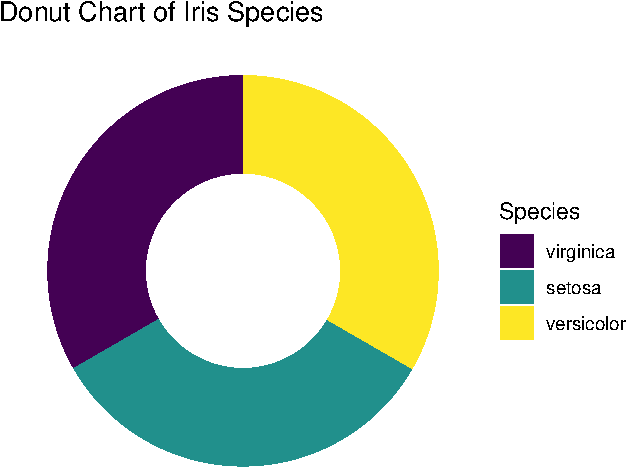
\includegraphics[keepaspectratio]{03_Data_Visualization_files/figure-pdf/fig-3-34-1.pdf}}

}

\caption{\label{fig-3-34}Piechart using \texttt{ggplot2} without no
background.}

\end{figure}%

\subsection{One Categorical and One Numeric
Variables}\label{one-categorical-and-one-numeric-variables-1}

\subsubsection{Side-by-side Box Plot}\label{side-by-side-box-plot-1}

Here you want to compare the robust statistics among different species.

\begin{Shaded}
\begin{Highlighting}[]
\FunctionTok{require}\NormalTok{(patchwork)}

\NormalTok{p1 }\OtherTok{\textless{}{-}} \FunctionTok{ggplot}\NormalTok{(}\AttributeTok{data=}\NormalTok{iris, }\FunctionTok{aes}\NormalTok{(}\AttributeTok{x=}\NormalTok{Species, }\AttributeTok{y=}\NormalTok{Sepal.Length)) }\SpecialCharTok{+}
        \FunctionTok{geom\_boxplot}\NormalTok{() }\SpecialCharTok{+}
        \FunctionTok{labs}\NormalTok{(}\AttributeTok{title =} \StringTok{"A Side{-}by{-}Side box plot"}\NormalTok{) }\SpecialCharTok{+}
        \FunctionTok{theme}\NormalTok{(}\AttributeTok{plot.title =} \FunctionTok{element\_text}\NormalTok{(}\AttributeTok{hjust =} \FloatTok{0.5}\NormalTok{))}

\NormalTok{p2 }\OtherTok{\textless{}{-}} \FunctionTok{ggplot}\NormalTok{(}\AttributeTok{data=}\NormalTok{iris, }\FunctionTok{aes}\NormalTok{(}\AttributeTok{x=}\NormalTok{Sepal.Length, }\AttributeTok{y=}\NormalTok{Species)) }\SpecialCharTok{+}
        \FunctionTok{geom\_boxplot}\NormalTok{() }\SpecialCharTok{+}
        \FunctionTok{labs}\NormalTok{(}\AttributeTok{title =} \StringTok{"A Horizontal Side{-}by{-}Side box plot"}\NormalTok{) }\SpecialCharTok{+}
        \FunctionTok{theme}\NormalTok{(}\AttributeTok{plot.title =} \FunctionTok{element\_text}\NormalTok{(}\AttributeTok{hjust =} \FloatTok{0.5}\NormalTok{))}

\NormalTok{p1}\SpecialCharTok{/}\NormalTok{p2}
\end{Highlighting}
\end{Shaded}

\begin{figure}[H]

\centering{

\pandocbounded{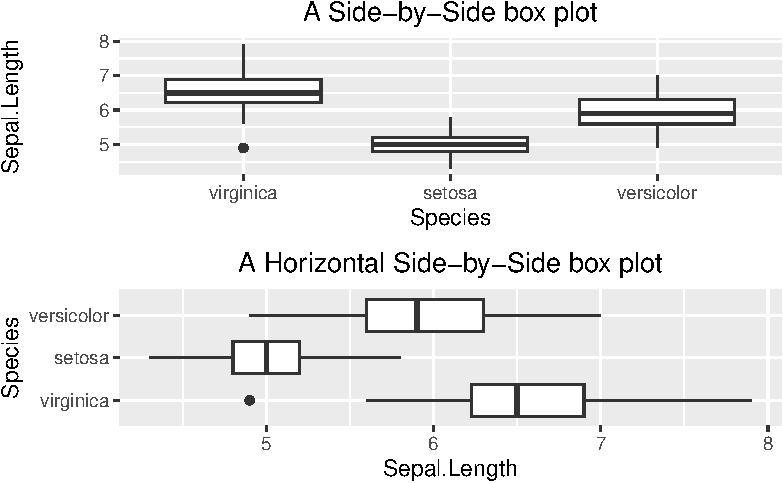
\includegraphics[keepaspectratio]{03_Data_Visualization_files/figure-pdf/fig-3-35-1.pdf}}

}

\caption{\label{fig-3-35}A side-by-side box plot}

\end{figure}%

\subsubsection{Side-by-side Bar Plot}\label{side-by-side-bar-plot-1}

Here, you want to compare the average \texttt{Sepal.Length} among iris
species. As discussed above, you calculate the averages and store them
in a separate table. It makes use of pipe, group by, and summarize
concepts discussed in Section~\ref{sec-tidyverse-tabulation}.

\begin{Shaded}
\begin{Highlighting}[]
\NormalTok{iris\_summary1 }\OtherTok{\textless{}{-}}\NormalTok{ iris }\SpecialCharTok{\%\textgreater{}\%}
                  \FunctionTok{group\_by}\NormalTok{(Species) }\SpecialCharTok{\%\textgreater{}\%}
                  \FunctionTok{summarize}\NormalTok{(}\AttributeTok{mean\_sepal\_length =} \FunctionTok{mean}\NormalTok{(Sepal.Length))}
\NormalTok{iris\_summary1}
\end{Highlighting}
\end{Shaded}

\begin{verbatim}
# A tibble: 3 x 2
  Species    mean_sepal_length
  <ord>                  <dbl>
1 virginica               6.59
2 setosa                  5.01
3 versicolor              5.94
\end{verbatim}

And then, you can plot the summary table. The geometry function is
\texttt{geom\_bar(stat\ =\ "identity")}. The
\texttt{stat\ =\ "identity"} parameter tells the \texttt{geom\_bar()}
function to set up the height of the bars according to the face value of
\texttt{mean\_sepal\_length}.

\begin{Shaded}
\begin{Highlighting}[]
\FunctionTok{ggplot}\NormalTok{(}\AttributeTok{data=}\NormalTok{iris\_summary1, }\FunctionTok{aes}\NormalTok{(}\AttributeTok{x=}\NormalTok{Species, }\AttributeTok{y=}\NormalTok{mean\_sepal\_length)) }\SpecialCharTok{+}
  \FunctionTok{geom\_bar}\NormalTok{(}\AttributeTok{stat =} \StringTok{"identity"}\NormalTok{) }\SpecialCharTok{+}
  \FunctionTok{labs}\NormalTok{(}\AttributeTok{x=}\StringTok{"Species"}\NormalTok{, }\AttributeTok{y=}\StringTok{"Average Sepal Length"}\NormalTok{, }\AttributeTok{title =} \StringTok{"Side{-}by{-}side Barplot"}\NormalTok{) }\SpecialCharTok{+}
  \FunctionTok{theme}\NormalTok{(}\AttributeTok{plot.title =} \FunctionTok{element\_text}\NormalTok{(}\AttributeTok{hjust =} \FloatTok{0.5}\NormalTok{))}
\end{Highlighting}
\end{Shaded}

\begin{figure}[H]

\centering{

\pandocbounded{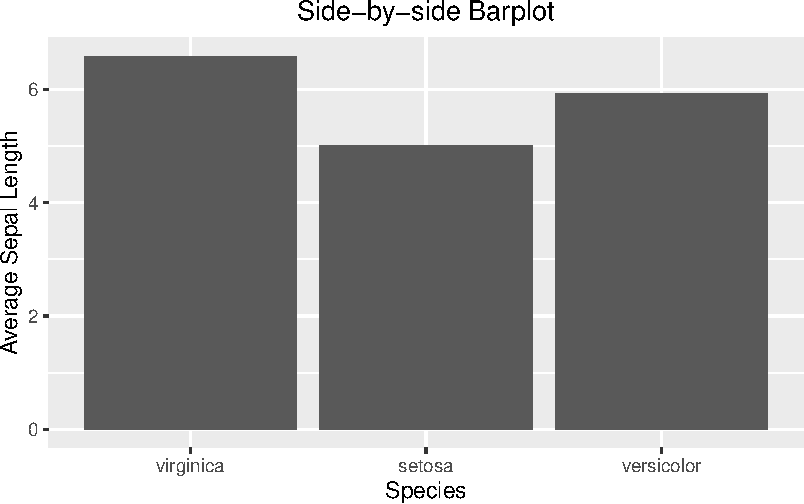
\includegraphics[keepaspectratio]{03_Data_Visualization_files/figure-pdf/fig-3-36-1.pdf}}

}

\caption{\label{fig-3-36}A side-by-side bar plot}

\end{figure}%

\subsubsection{Side-by-side Bar Plot with Error
Bar}\label{sec-ggplot-error-bar}

The calculation of the error bar (i.e., the standard error \texttt{se})
requires standard deviation and sample size. Once \texttt{se} is
calculated, it can be used to calculate the minimum (lower) and maximum
(upper) of the error bar.

\begin{Shaded}
\begin{Highlighting}[]
\NormalTok{iris\_summary2 }\OtherTok{\textless{}{-}}\NormalTok{ iris }\SpecialCharTok{\%\textgreater{}\%}
                  \FunctionTok{group\_by}\NormalTok{(Species) }\SpecialCharTok{\%\textgreater{}\%}
                  \FunctionTok{summarize}\NormalTok{(}\AttributeTok{mean\_sepal\_length =} \FunctionTok{mean}\NormalTok{(Sepal.Length),}
                            \AttributeTok{N=}\FunctionTok{n}\NormalTok{(),}
                            \AttributeTok{se=}\FunctionTok{sd}\NormalTok{(Sepal.Length)}\SpecialCharTok{/}\FunctionTok{sqrt}\NormalTok{(N)) }\SpecialCharTok{\%\textgreater{}\%}
                  \CommentTok{\# add the y minimum and y maximum columns}
                  \FunctionTok{mutate}\NormalTok{(}\AttributeTok{ymin =}\NormalTok{ mean\_sepal\_length }\SpecialCharTok{{-}}\NormalTok{ se,}
                         \AttributeTok{ymax =}\NormalTok{ mean\_sepal\_length }\SpecialCharTok{+}\NormalTok{ se)}
\NormalTok{iris\_summary2}
\end{Highlighting}
\end{Shaded}

\begin{verbatim}
# A tibble: 3 x 6
  Species    mean_sepal_length     N     se  ymin  ymax
  <ord>                  <dbl> <int>  <dbl> <dbl> <dbl>
1 virginica               6.59    50 0.0899  6.50  6.68
2 setosa                  5.01    50 0.0498  4.96  5.06
3 versicolor              5.94    50 0.0730  5.86  6.01
\end{verbatim}

\begin{Shaded}
\begin{Highlighting}[]
\FunctionTok{ggplot}\NormalTok{(}\AttributeTok{data=}\NormalTok{iris\_summary2, }\FunctionTok{aes}\NormalTok{(}\AttributeTok{x=}\NormalTok{Species, }\AttributeTok{y=}\NormalTok{mean\_sepal\_length)) }\SpecialCharTok{+}
  \FunctionTok{geom\_bar}\NormalTok{(}\AttributeTok{stat =} \StringTok{"identity"}\NormalTok{) }\SpecialCharTok{+}
  \FunctionTok{geom\_errorbar}\NormalTok{(}\FunctionTok{aes}\NormalTok{(}\AttributeTok{ymin =}\NormalTok{ ymin, }\AttributeTok{ymax =}\NormalTok{ ymax), }\AttributeTok{width =} \FloatTok{0.2}\NormalTok{, }\AttributeTok{color=}\StringTok{\textquotesingle{}red\textquotesingle{}}\NormalTok{) }\SpecialCharTok{+}
  \FunctionTok{labs}\NormalTok{(}\AttributeTok{x=}\StringTok{"Species"}\NormalTok{, }\AttributeTok{y=}\StringTok{"Average Sepal Length"}\NormalTok{, }\AttributeTok{title =} \StringTok{"Side{-}by{-}side Barplot"}\NormalTok{) }\SpecialCharTok{+}
  \FunctionTok{theme}\NormalTok{(}\AttributeTok{plot.title =} \FunctionTok{element\_text}\NormalTok{(}\AttributeTok{hjust =} \FloatTok{0.5}\NormalTok{))}
\end{Highlighting}
\end{Shaded}

\begin{figure}[H]

\centering{

\pandocbounded{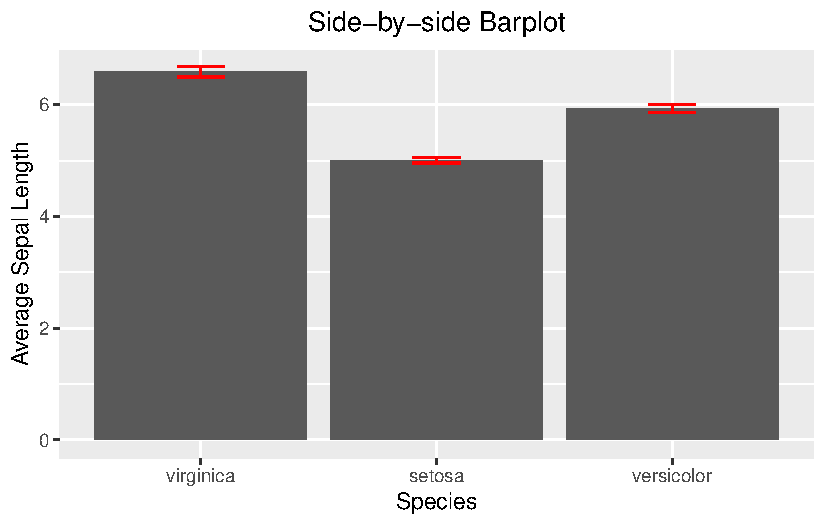
\includegraphics[keepaspectratio]{03_Data_Visualization_files/figure-pdf/fig-3-37-1.pdf}}

}

\caption{\label{fig-3-37}A side-by-side bar plot with error bar.}

\end{figure}%

\subsubsection{Line Graph with Error
Bar}\label{line-graph-with-error-bar-1}

Calculate the SE as above:

\begin{Shaded}
\begin{Highlighting}[]
\NormalTok{iris\_summary3 }\OtherTok{\textless{}{-}}\NormalTok{ iris }\SpecialCharTok{\%\textgreater{}\%}
                  \FunctionTok{group\_by}\NormalTok{(Species) }\SpecialCharTok{\%\textgreater{}\%}
                  \FunctionTok{summarize}\NormalTok{(}\AttributeTok{mean\_sepal\_length =} \FunctionTok{mean}\NormalTok{(Sepal.Length),}
                            \AttributeTok{N=}\FunctionTok{n}\NormalTok{(),}
                            \AttributeTok{se=}\FunctionTok{sd}\NormalTok{(Sepal.Length)}\SpecialCharTok{/}\FunctionTok{sqrt}\NormalTok{(N)) }\SpecialCharTok{\%\textgreater{}\%}
                  \FunctionTok{mutate}\NormalTok{(}\AttributeTok{ymin=}\NormalTok{mean\_sepal\_length}\SpecialCharTok{{-}}\NormalTok{se,}
                         \AttributeTok{ymax=}\NormalTok{mean\_sepal\_length}\SpecialCharTok{+}\NormalTok{se)}
\NormalTok{iris\_summary3}
\end{Highlighting}
\end{Shaded}

\begin{verbatim}
# A tibble: 3 x 6
  Species    mean_sepal_length     N     se  ymin  ymax
  <ord>                  <dbl> <int>  <dbl> <dbl> <dbl>
1 virginica               6.59    50 0.0899  6.50  6.68
2 setosa                  5.01    50 0.0498  4.96  5.06
3 versicolor              5.94    50 0.0730  5.86  6.01
\end{verbatim}

Incorporate the SE into a line plot.

\begin{Shaded}
\begin{Highlighting}[]
\FunctionTok{ggplot}\NormalTok{(iris\_summary3, }\FunctionTok{aes}\NormalTok{(}\AttributeTok{x=}\NormalTok{Species, }\AttributeTok{y=}\NormalTok{mean\_sepal\_length, }\AttributeTok{group =} \DecValTok{1}\NormalTok{)) }\SpecialCharTok{+}
  \FunctionTok{geom\_line}\NormalTok{(}\AttributeTok{color =} \StringTok{\textquotesingle{}skyblue\textquotesingle{}}\NormalTok{) }\SpecialCharTok{+}
  \FunctionTok{geom\_point}\NormalTok{(}\AttributeTok{size =} \DecValTok{3}\NormalTok{, }\AttributeTok{color =} \StringTok{\textquotesingle{}skyblue\textquotesingle{}}\NormalTok{) }\SpecialCharTok{+}
  \FunctionTok{geom\_errorbar}\NormalTok{(}\FunctionTok{aes}\NormalTok{(}\AttributeTok{ymin =}\NormalTok{ ymin, }\AttributeTok{ymax =}\NormalTok{ ymax), }\AttributeTok{width =} \FloatTok{0.1}\NormalTok{, }\AttributeTok{linewidth =} \DecValTok{1}\NormalTok{) }\SpecialCharTok{+}
  \FunctionTok{labs}\NormalTok{(}\AttributeTok{x=}\StringTok{"Species"}\NormalTok{, }\AttributeTok{y=}\StringTok{"Sepal Length"}\NormalTok{, }\AttributeTok{title =} \StringTok{"Line Plot with Erorr Bar"}\NormalTok{) }\SpecialCharTok{+}
  \FunctionTok{theme}\NormalTok{(}\AttributeTok{plot.title =} \FunctionTok{element\_text}\NormalTok{(}\AttributeTok{hjust =} \FloatTok{0.5}\NormalTok{))}
\end{Highlighting}
\end{Shaded}

\begin{figure}[H]

\centering{

\pandocbounded{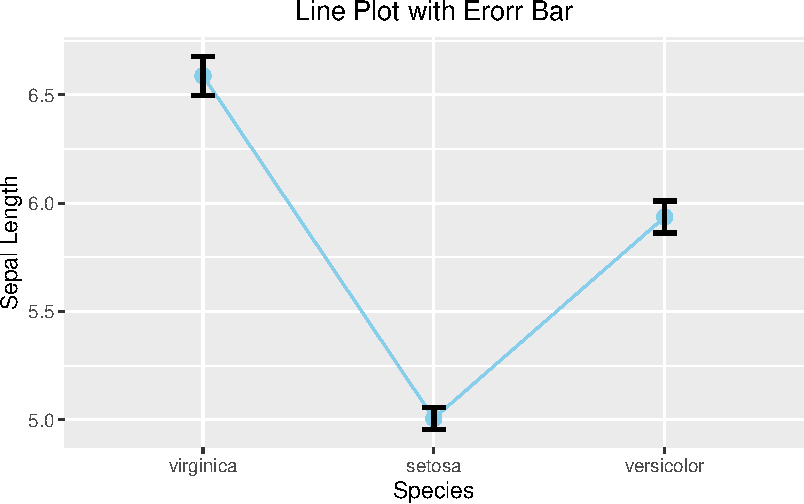
\includegraphics[keepaspectratio]{03_Data_Visualization_files/figure-pdf/fig-3-38-1.pdf}}

}

\caption{\label{fig-3-38}A line plot with error bar.}

\end{figure}%

\subsubsection{Overlapping
Histogram}\label{sec-ggplot-overlapping-histogram}

Like the base R side-by-side histogram, you will set the transparency to
0.5 and bin width to 0.25. Note that there is no need to care about the
x- and y-limit in \texttt{ggplot2}.

\begin{Shaded}
\begin{Highlighting}[]
\FunctionTok{ggplot}\NormalTok{(}\AttributeTok{data=}\NormalTok{iris, }\FunctionTok{aes}\NormalTok{(}\AttributeTok{x=}\NormalTok{Sepal.Length, }\AttributeTok{fill=}\NormalTok{Species)) }\SpecialCharTok{+}
  \FunctionTok{geom\_histogram}\NormalTok{(}\AttributeTok{alpha=}\FloatTok{0.5}\NormalTok{, }\AttributeTok{binwidth =} \FloatTok{0.25}\NormalTok{) }\SpecialCharTok{+}
  \FunctionTok{labs}\NormalTok{(}\AttributeTok{x=}\StringTok{"Sepal Length"}\NormalTok{, }\AttributeTok{title =} \StringTok{"Overlapping Histogram"}\NormalTok{) }\SpecialCharTok{+}
  \FunctionTok{theme}\NormalTok{(}\AttributeTok{plot.title =} \FunctionTok{element\_text}\NormalTok{(}\AttributeTok{hjust =} \FloatTok{0.5}\NormalTok{))}
\end{Highlighting}
\end{Shaded}

\begin{figure}[H]

\centering{

\pandocbounded{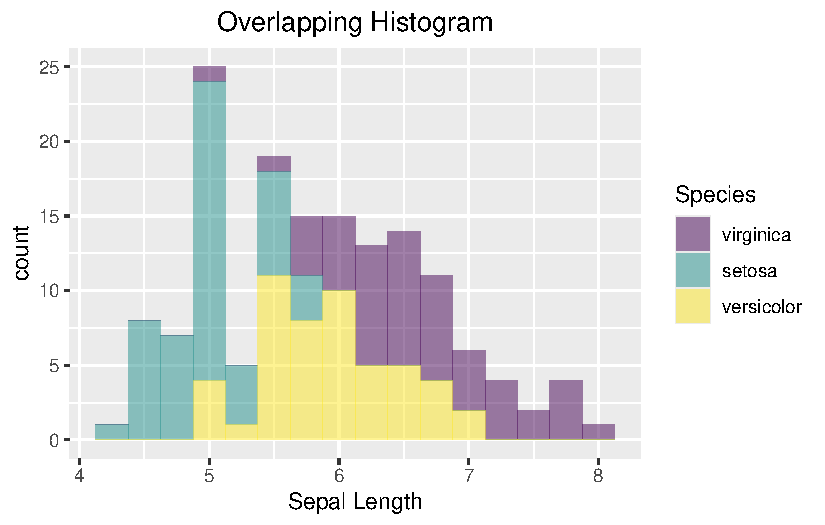
\includegraphics[keepaspectratio]{03_Data_Visualization_files/figure-pdf/fig-3-39-1.pdf}}

}

\caption{\label{fig-3-39}A side-by-side histogram.}

\end{figure}%

\subsection{Contingency Table}\label{contingency-table-1}

The \texttt{penguins} data set is used to illustrate how to create a
side-by-side bar plot or a mosaic plot for displaying count data.

First, let's create a contingency table as below:

\begin{Shaded}
\begin{Highlighting}[]
\NormalTok{mytab }\OtherTok{\textless{}{-}} \FunctionTok{with}\NormalTok{(penguins, }\FunctionTok{table}\NormalTok{(species, island))}
\NormalTok{mytab}
\end{Highlighting}
\end{Shaded}

\begin{verbatim}
           island
species     Biscoe Dream Torgersen
  Adelie        44    56        52
  Chinstrap      0    68         0
  Gentoo       124     0         0
\end{verbatim}

As \texttt{ggplot2} only works with data frames, \texttt{mytab} is
\textbf{not} a data frame. Therefore, the first step is to convert the
contingency table into a data frame.

\begin{Shaded}
\begin{Highlighting}[]
\NormalTok{mydf }\OtherTok{\textless{}{-}} \FunctionTok{as.data.frame}\NormalTok{(mytab)}
\FunctionTok{colnames}\NormalTok{(mydf) }\OtherTok{\textless{}{-}} \FunctionTok{c}\NormalTok{(}\StringTok{"species"}\NormalTok{,}\StringTok{"island"}\NormalTok{,}\StringTok{"Count"}\NormalTok{)}
\NormalTok{mydf}
\end{Highlighting}
\end{Shaded}

\begin{verbatim}
    species    island Count
1    Adelie    Biscoe    44
2 Chinstrap    Biscoe     0
3    Gentoo    Biscoe   124
4    Adelie     Dream    56
5 Chinstrap     Dream    68
6    Gentoo     Dream     0
7    Adelie Torgersen    52
8 Chinstrap Torgersen     0
9    Gentoo Torgersen     0
\end{verbatim}

Now we can plot \texttt{mydf}.

\begin{Shaded}
\begin{Highlighting}[]
\FunctionTok{ggplot}\NormalTok{(}\AttributeTok{data=}\NormalTok{mydf, }\FunctionTok{aes}\NormalTok{(}\AttributeTok{x=}\NormalTok{island, }\AttributeTok{y=}\NormalTok{Count, }\AttributeTok{fill=}\NormalTok{species)) }\SpecialCharTok{+}
  \FunctionTok{geom\_col}\NormalTok{(}\AttributeTok{position =} \StringTok{"dodge"}\NormalTok{) }\SpecialCharTok{+}
  \FunctionTok{labs}\NormalTok{(}\AttributeTok{title =} \StringTok{"Side{-}by{-}side Barplot"}\NormalTok{, }\AttributeTok{x =} \StringTok{"Island"}\NormalTok{, }\AttributeTok{y =} \StringTok{"Count"}\NormalTok{)}
\end{Highlighting}
\end{Shaded}

\begin{figure}[H]

\centering{

\pandocbounded{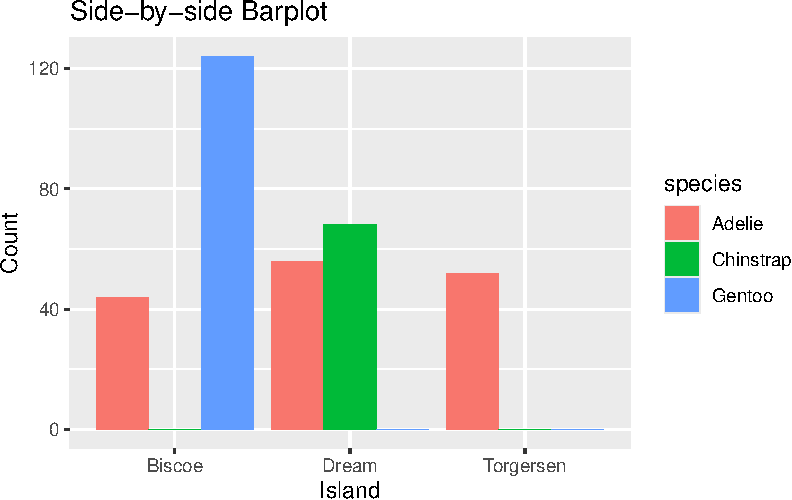
\includegraphics[keepaspectratio]{03_Data_Visualization_files/figure-pdf/fig-3-40-1.pdf}}

}

\caption{\label{fig-3-40}Plotting a contingency table using a
side-by-side bar plot.}

\end{figure}%

\subsection{Two Numeric Variables}\label{two-numeric-variables-1}

Use a scatter plot to visualize the relationship between two numeric
variables. As said above, the revealed relationship can be linear and
non-linear.

\begin{Shaded}
\begin{Highlighting}[]
\FunctionTok{ggplot}\NormalTok{(iris, }\FunctionTok{aes}\NormalTok{(}\AttributeTok{x=}\NormalTok{Sepal.Width, }\AttributeTok{y=}\NormalTok{Sepal.Length)) }\SpecialCharTok{+}
  \FunctionTok{geom\_point}\NormalTok{() }\SpecialCharTok{+}
  \FunctionTok{labs}\NormalTok{(}\AttributeTok{x=}\StringTok{"Sepal Width"}\NormalTok{, }\AttributeTok{y=}\StringTok{"Sepal Length"}\NormalTok{, }\AttributeTok{title =} \StringTok{"A Scatter Plot"}\NormalTok{) }\SpecialCharTok{+}
  \FunctionTok{theme}\NormalTok{(}\AttributeTok{plot.title =} \FunctionTok{element\_text}\NormalTok{(}\AttributeTok{hjust =} \FloatTok{0.5}\NormalTok{))}
\end{Highlighting}
\end{Shaded}

\begin{figure}[H]

\centering{

\pandocbounded{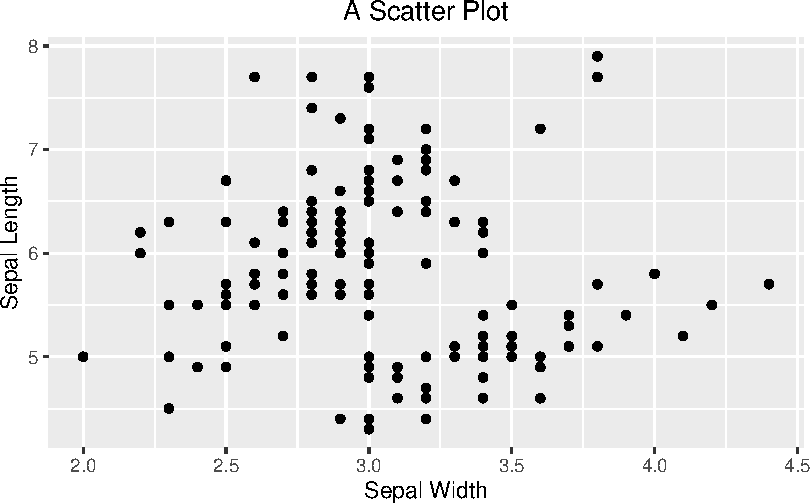
\includegraphics[keepaspectratio]{03_Data_Visualization_files/figure-pdf/fig-3-42-1.pdf}}

}

\caption{\label{fig-3-42}Visualizing the relationship between two
numeric variables using a scatter plot.}

\end{figure}%

If you wanted to emphasize their linear relationship, it can be done
convincingly by adding a regression line on top of the scatter plot.
\texttt{ggplot2} spares you the effort to create a linear model like
base R. Instead, it can be done by adding the \texttt{geom\_smooth()}.
You tell
\texttt{geom\_smooth(method\ =\ "lm",\ se\ =\ FALSE,\ color\ =\ "red")}
to use a linear method (\texttt{lm}) for smoothing the data points. See
the code below:

\begin{Shaded}
\begin{Highlighting}[]
\FunctionTok{ggplot}\NormalTok{(iris, }\FunctionTok{aes}\NormalTok{(}\AttributeTok{x=}\NormalTok{Sepal.Width, }\AttributeTok{y=}\NormalTok{Sepal.Length)) }\SpecialCharTok{+}
  \FunctionTok{geom\_point}\NormalTok{() }\SpecialCharTok{+}
  \FunctionTok{geom\_smooth}\NormalTok{(}\AttributeTok{method =} \StringTok{"lm"}\NormalTok{, }\AttributeTok{se =} \ConstantTok{FALSE}\NormalTok{, }\AttributeTok{color =} \StringTok{"red"}\NormalTok{) }\SpecialCharTok{+}
  \FunctionTok{labs}\NormalTok{(}\AttributeTok{x=}\StringTok{"Sepal Width"}\NormalTok{, }\AttributeTok{y=}\StringTok{"Sepal Length"}\NormalTok{, }\AttributeTok{title =} \StringTok{"Scatter Plot with the Regression Line"}\NormalTok{) }\SpecialCharTok{+}
  \FunctionTok{theme}\NormalTok{(}\AttributeTok{plot.title =} \FunctionTok{element\_text}\NormalTok{(}\AttributeTok{hjust =} \FloatTok{0.5}\NormalTok{))}
\end{Highlighting}
\end{Shaded}

\begin{verbatim}
`geom_smooth()` using formula = 'y ~ x'
\end{verbatim}

\begin{figure}[H]

\centering{

\pandocbounded{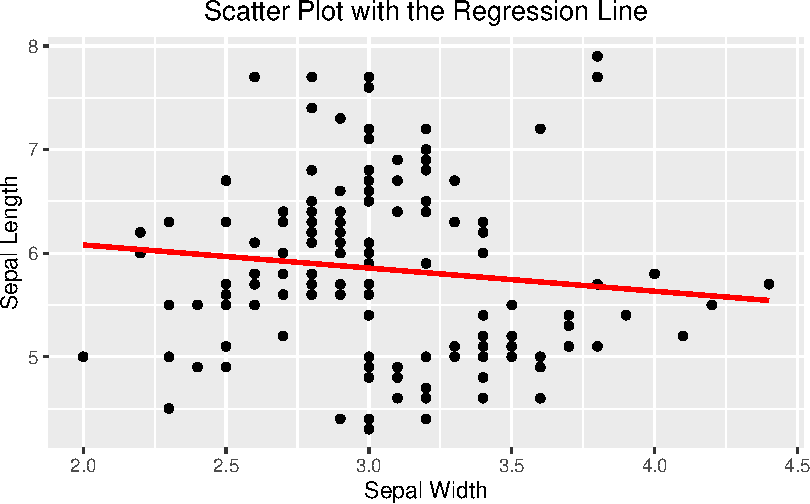
\includegraphics[keepaspectratio]{03_Data_Visualization_files/figure-pdf/fig-3-43-1.pdf}}

}

\caption{\label{fig-3-43}A scatter plot overlaid with a regression
line.}

\end{figure}%

If you see this message ``\texttt{geom\_smooth()} using formula = `y
\textasciitilde{} x'\,'', it is harmless, and informational.
\texttt{ggplot2} is just to let you know what the response and predictor
are used by \texttt{geom\_smooth()} in creating the regression line.

\subsection{Multipanel Scatter Plot}\label{multipanel-scatter-plot-1}

Often times before multiple linear regression, it is recommended to
visualize the relationship between the response variable and the
independent variables pairwisely, or the linear relationship between
independent variables. The latter is important, as it may cause the
\textbf{collinearity} issue if independent variables are linearly
correlated.

A multipanel scatter plot can do this. However, \texttt{ggplot2} does
not have a geometry function for it. The simplest way is to use the
\texttt{ggpairs()} function provided by the \texttt{GGally} package,
which requires installation, if you have not done so.

Suppose, you are interested in the pairwise relationship between all
numeric variables in \texttt{iris}. It can easily be done using the
\texttt{ggpairs()} plot function. Color is the attribute used to
distinguish species. \texttt{progress\ =\ FALSE} is to suppress the
printing of the progress bar.

\begin{Shaded}
\begin{Highlighting}[]
\FunctionTok{library}\NormalTok{(GGally)}
\FunctionTok{ggpairs}\NormalTok{(iris, }\FunctionTok{aes}\NormalTok{(}\AttributeTok{color =}\NormalTok{ Species), }\AttributeTok{title =} \StringTok{"A Multi{-}panel Scatter Plot"}\NormalTok{, }\AttributeTok{progress =} \ConstantTok{FALSE}\NormalTok{)}
\end{Highlighting}
\end{Shaded}

\begin{figure}[H]

\centering{

\pandocbounded{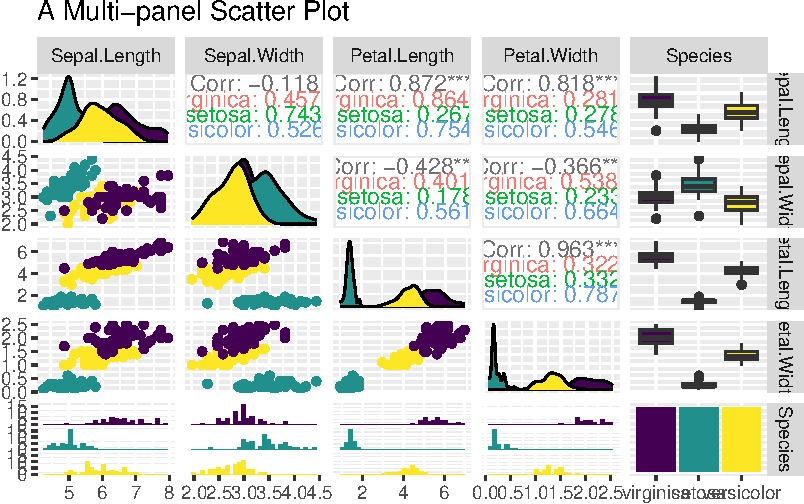
\includegraphics[keepaspectratio]{03_Data_Visualization_files/figure-pdf/fig-3-44-1.pdf}}

}

\caption{\label{fig-3-44}A Multipanel Scatter Plot}

\end{figure}%

\section{Summary}\label{summary-2}

This is big chapter that has discussed an array of plot functions both
from base R and \texttt{ggplot2}. It is more like a cookbook of various
visualization recipes. So, instead of listing all the functions here, it
is helpful to list several useful resources that you can fine-tune the
graphs yourselves.

\textbf{pch}

If you type \texttt{help(pch)} at the console, R shows the \texttt{pch}
section of the help page for \texttt{points}. Below is a snapshot of
\texttt{pch} values and the corresponding plotting characters:

\begin{figure}

\centering{

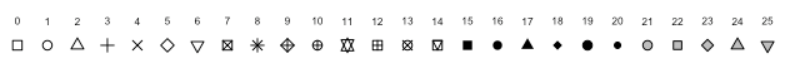
\includegraphics[width=0.8\linewidth,height=0.8\textheight]{images/pch_symbols.png}

}

\caption{\label{fig-3-45}\texttt{pch} values}

\end{figure}%

\textbf{Color}

R supports a large number of colors and palettes.
\href{https://r-graph-gallery.com/colors.html}{R Graph Gallery} is a
great resource to see what choices are available and their names .

\part{Part II}

\chapter{Statistical Tests}\label{sec-04-statistical-tests}

R was inherently designed for statistical analysis. Therefore, it is
justified to devote a chapter to statistical tests. Here, we will
discuss a list of classic statistical tests with an emphasis on the Null
Hypothesis Significance Test (NHST). While understanding the core
principles of the tests is essential, this chapter, as well as the whole
book, emphasizes using R; as such, the underlying concepts of the tests
are omitted. There are many excellent open introductory statistics
textbooks\footnote{Introductory Statistics for Life and Biomedical
  Sciences: \url{https://openintro.org/book/biostat/}} \footnote{Introduction
  to Modern Statistics: \url{https://openintro.org/book/ims/}}
\footnote{Handbook of Biological Statistics:
  \url{https://www.biostathandbook.com/}}. Interested readers should
consult them for further detail.

\section*{Learning Objectives:}\label{learning-objectives-3}
\addcontentsline{toc}{section}{Learning Objectives:}

\markright{Learning Objectives:}

\begin{itemize}
\item
  Test a quantitative variable in one, two, or more groups.
\item
  Test for one or two categorical variables.
\item
  Linear regression
\end{itemize}

\section{Data Set}\label{data-set}

We will use a new data set for this chapter. Follow the steps below to
import the data set \texttt{FlightDelays} into RStudio.

\begin{Shaded}
\begin{Highlighting}[]
\ControlFlowTok{if}\NormalTok{ (}\SpecialCharTok{!}\FunctionTok{require}\NormalTok{(resampledata)) \{}
  \FunctionTok{install.packages}\NormalTok{(}\StringTok{\textquotesingle{}resampledata\textquotesingle{}}\NormalTok{)}
\NormalTok{\}}
\end{Highlighting}
\end{Shaded}

\begin{verbatim}
Loading required package: resampledata
\end{verbatim}

\begin{verbatim}

Attaching package: 'resampledata'
\end{verbatim}

\begin{verbatim}
The following object is masked from 'package:datasets':

    Titanic
\end{verbatim}

\begin{Shaded}
\begin{Highlighting}[]
\FunctionTok{require}\NormalTok{(resampledata)}
\FunctionTok{data}\NormalTok{(FlightDelays)}
\end{Highlighting}
\end{Shaded}

Take a glimpse of the data set.

\begin{Shaded}
\begin{Highlighting}[]
\FunctionTok{summary}\NormalTok{(FlightDelays)}
\end{Highlighting}
\end{Shaded}

\begin{verbatim}
       ID       Carrier      FlightNo      Destination    DepartTime  
 Min.   :   1   AA:2906   Min.   :  71.0   BNA: 172    4-8am   : 699  
 1st Qu.:1008   UA:1123   1st Qu.: 371.0   DEN: 264    8-Noon  :1053  
 Median :2015             Median : 691.0   DFW: 918    Noon-4pm:1048  
 Mean   :2015             Mean   : 827.1   IAD:  55    4-8pm   : 972  
 3rd Qu.:3022             3rd Qu.: 787.0   MIA: 610    8-Mid   : 257  
 Max.   :4029             Max.   :2255.0   ORD:1785                   
                                           STL: 225                   
  Day       Month       FlightLength       Delay        Delayed30 
 Sun:551   May :1999   Min.   : 68.0   Min.   :-19.00   No :3432  
 Mon:630   June:2030   1st Qu.:155.0   1st Qu.: -6.00   Yes: 597  
 Tue:628               Median :163.0   Median : -3.00             
 Wed:564               Mean   :185.3   Mean   : 11.74             
 Thu:566               3rd Qu.:228.0   3rd Qu.:  5.00             
 Fri:637               Max.   :295.0   Max.   :693.00             
 Sat:453                                                          
\end{verbatim}

It contains 10 variables, out of which two are quantitative variables
(\texttt{FlightLength}, and \texttt{Delay}), and the rest are
categorical variables. Notice that there is a glitch: R mistakenly
considered \texttt{FlightNo} as a quantitative variable. However, it
does not affect us, as we do not use this variable here. If you want to
convert it to a categorical variable (factor), here is the step:

\begin{Shaded}
\begin{Highlighting}[]
\NormalTok{FlightDelays}\SpecialCharTok{$}\NormalTok{FlightNo }\OtherTok{\textless{}{-}} \FunctionTok{as.factor}\NormalTok{(FlightDelays}\SpecialCharTok{$}\NormalTok{FlightNo)}
\end{Highlighting}
\end{Shaded}

\section{Tests for Quantitative
Variables}\label{tests-for-quantitative-variables}

\subsection{One-sample t-tests}\label{one-sample-t-tests}

The goal of a one-sample t-test is to test if the mean of a quantitative
variable is equal to a certain value. For example, if the aviation
regulatory agency states that acceptable flight delay is 12 minutes. We
want to see if the flights meet the requirement. The null hypothesis
(\$H\_\{0\}\$) is that the mean delay is equal to 12 minutes. The
alternative hypothesis (\$H\_\{A\}\$) is that the mean delay is not
equal to 12 minutes. Here are the steps to perform such a test:

\begin{Shaded}
\begin{Highlighting}[]
\FunctionTok{t.test}\NormalTok{(FlightDelays}\SpecialCharTok{$}\NormalTok{Delay, }\AttributeTok{mu =} \DecValTok{12}\NormalTok{)}
\end{Highlighting}
\end{Shaded}

\begin{verbatim}

    One Sample t-test

data:  FlightDelays$Delay
t = -0.39963, df = 4028, p-value = 0.6895
alternative hypothesis: true mean is not equal to 12
95 percent confidence interval:
 10.45205 13.02375
sample estimates:
mean of x 
  11.7379 
\end{verbatim}

As the p-value (0.6895) is greater than \(\alpha\) = 0.05 at a 95\%
confidence level, we fail to reject the null \(H_{0}\), meaning that the
mean flight delay meets the standard.

\subsection{Two-sample t-tests}\label{two-sample-t-tests}

A two-sample t-test tests whether the mean of one group is the same as
the other group. The \(H_{0}\) states the two groups have the same mean,
and the \(H_{A}\) states otherwise.

For example, we want to compare the mean delay of the two carriers to
determine whether they are the same.

\emph{Solution 1:}

\begin{Shaded}
\begin{Highlighting}[]
\NormalTok{AA\_delay }\OtherTok{\textless{}{-}} \FunctionTok{subset}\NormalTok{(FlightDelays, Carrier}\SpecialCharTok{==}\StringTok{"AA"}\NormalTok{)}
\NormalTok{UA\_delay }\OtherTok{\textless{}{-}} \FunctionTok{subset}\NormalTok{(FlightDelays, Carrier}\SpecialCharTok{==}\StringTok{"UA"}\NormalTok{)}
\FunctionTok{t.test}\NormalTok{(AA\_delay}\SpecialCharTok{$}\NormalTok{Delay, UA\_delay}\SpecialCharTok{$}\NormalTok{Delay)}
\end{Highlighting}
\end{Shaded}

\begin{verbatim}

    Welch Two Sample t-test

data:  AA_delay$Delay and UA_delay$Delay
t = -3.8255, df = 1843.8, p-value = 0.0001349
alternative hypothesis: true difference in means is not equal to 0
95 percent confidence interval:
 -8.903198 -2.868194
sample estimates:
mean of x mean of y 
 10.09738  15.98308 
\end{verbatim}

Based on the p-value (0.0001349) being less than \(\alpha\) = 0.05, the
delays of the two carriers are different. The bottom of the test result
shows that the mean delay of 10.09738 for AA (group x) is shorter than
UA 15.98308.

\emph{Solution 2:}

This approach makes use of the categorical variable \texttt{carrier} to
split the data set into two, avoiding the creation of two temporary data
frames.

\begin{Shaded}
\begin{Highlighting}[]
\FunctionTok{t.test}\NormalTok{(Delay }\SpecialCharTok{\textasciitilde{}}\NormalTok{ Carrier, }\AttributeTok{data=}\NormalTok{FlightDelays)}
\end{Highlighting}
\end{Shaded}

\begin{verbatim}

    Welch Two Sample t-test

data:  Delay by Carrier
t = -3.8255, df = 1843.8, p-value = 0.0001349
alternative hypothesis: true difference in means between group AA and group UA is not equal to 0
95 percent confidence interval:
 -8.903198 -2.868194
sample estimates:
mean in group AA mean in group UA 
        10.09738         15.98308 
\end{verbatim}

The symbol \texttt{\textasciitilde{}} means ``split by''.
\texttt{Delay\ \textasciitilde{}\ Carrier} means to split \texttt{Delay}
by \texttt{Carrier}.

\subsection{One-way ANOVA}\label{one-way-anova}

A one-way ANOVA test tests whether the means of three or more groups are
the same or not. Two key differences from the two-sample t-test above:
1. a two-sample t-test can handle only two groups, but ANOVA can handle
two or more groups. 2. The \(H_{0}\) of ANOVA is rejected if any pair(s)
of groups have unequal means.

For example, test whether mean delays vary by destination.

\begin{Shaded}
\begin{Highlighting}[]
\NormalTok{aov\_results }\OtherTok{\textless{}{-}} \FunctionTok{aov}\NormalTok{(Delay }\SpecialCharTok{\textasciitilde{}}\NormalTok{ Destination, }\AttributeTok{data=}\NormalTok{FlightDelays)}
\FunctionTok{summary}\NormalTok{(aov\_results)}
\end{Highlighting}
\end{Shaded}

\begin{verbatim}
              Df  Sum Sq Mean Sq F value   Pr(>F)    
Destination    6   62891   10482   6.094 2.29e-06 ***
Residuals   4022 6918028    1720                     
---
Signif. codes:  0 '***' 0.001 '**' 0.01 '*' 0.05 '.' 0.1 ' ' 1
\end{verbatim}

If you only care whether the \(H_{0}\) can be rejected, focus on the
overall p-value (2.29e-06) under the \texttt{Pr(\textgreater{}F)} column
on the right. It is undeniably smaller than \(\alpha\) = 0.05, so the
\(H_{0}\) can be rejected.

In some situations, you may be interested in finding out which pair(s)
do not have the same mean. Tukey's Honest Significant Difference (HSD)
test can answer this question.

\begin{Shaded}
\begin{Highlighting}[]
\FunctionTok{TukeyHSD}\NormalTok{(aov\_results)}
\end{Highlighting}
\end{Shaded}

\begin{verbatim}
  Tukey multiple comparisons of means
    95% family-wise confidence level

Fit: aov(formula = Delay ~ Destination, data = FlightDelays)

$Destination
               diff         lwr        upr     p adj
DEN-BNA   7.1454369  -4.8424432 19.1333171 0.5765602
DFW-BNA   3.2646932  -6.8999706 13.4293570 0.9647119
IAD-BNA  19.4461945   0.4951700 38.3972191 0.0399134
MIA-BNA  12.9137057   2.3518660 23.4755453 0.0058064
ORD-BNA   8.4338186  -1.3335463 18.2011835 0.1430105
STL-BNA   0.9181137 -11.4728506 13.3090780 0.9999910
DFW-DEN  -3.8807437 -12.4245377  4.6630503 0.8331281
IAD-DEN  12.3007576  -5.8325642 30.4340793 0.4140643
MIA-DEN   5.7682688  -3.2444158 14.7809533 0.4884472
ORD-DEN   1.2883817  -6.7786774  9.3554408 0.9991892
STL-DEN  -6.2273232 -17.3274143  4.8727678 0.6463375
IAD-DFW  16.1815013  -0.8016809 33.1646835 0.0736782
MIA-DFW   9.6490125   3.2584254 16.0395995 0.0001755
ORD-DFW   5.1691254   0.2003667 10.1378841 0.0352035
STL-DFW  -2.3465795 -11.4473015  6.7541425 0.9885164
MIA-IAD  -6.5324888 -23.7563253 10.6913477 0.9225580
ORD-IAD -11.0123759 -27.7607938  5.7360421 0.4540417
STL-IAD -18.5280808 -36.9303655 -0.1257961 0.0471723
ORD-MIA  -4.4798870 -10.2175372  1.2577631 0.2425378
STL-MIA -11.9955920 -21.5378772 -2.4533067 0.0039784
STL-ORD  -7.5157049 -16.1704244  1.1390145 0.1382159
\end{verbatim}

It lists all possible pairs of destinations. Since there are seven
destinations, the total number of pairs is 21 (\texttt{choose(7,2)}).

Each row shows the difference of means (\texttt{diff}), the lower
(\texttt{lwr}) and upper (\texttt{upr}) bounds of the confidence
interval, and the adjusted p-value (\texttt{p\ adj}). Examining the
p-value is the quickest way to identify pairs with unequal means. E.g.,
IAD-BNA in which the p-value is less than 0.05.

To ease analysis, it is suggested to plot the HSD result as below:

\begin{Shaded}
\begin{Highlighting}[]
\NormalTok{hsd\_results }\OtherTok{\textless{}{-}} \FunctionTok{TukeyHSD}\NormalTok{(aov\_results)}

\CommentTok{\# las=1 causes the plot to print the pair name horizontally.}
\FunctionTok{plot}\NormalTok{(hsd\_results, }\AttributeTok{las=}\DecValTok{1}\NormalTok{)}
\end{Highlighting}
\end{Shaded}

\pandocbounded{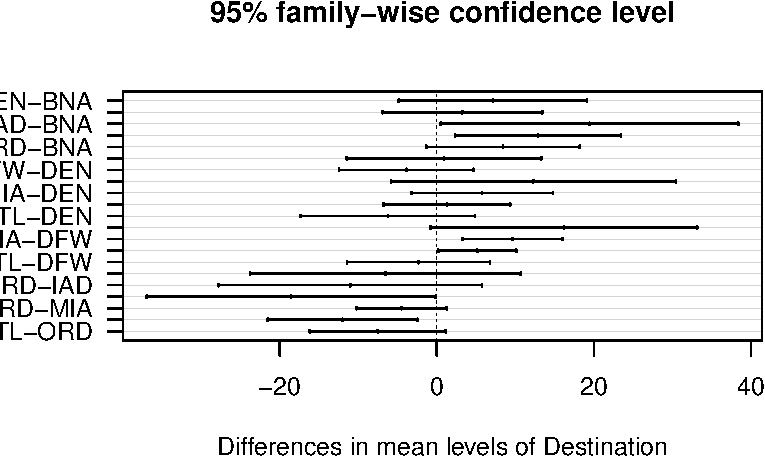
\includegraphics[keepaspectratio]{04_Statistical_Tests_files/figure-pdf/unnamed-chunk-9-1.pdf}}

Confidence intervals not crossing zero (the vertical line) indicate
pairs have unequal means.

\section{Tests for Categorical
Variables}\label{tests-for-categorical-variables}

\subsection{One Categorical Variable}\label{one-categorical-variable-2}

\subsection{Two Categorical Variables}\label{two-categorical-variables}

\section{Regression}\label{regression}

\subsection{Simple Linear Regression}\label{simple-linear-regression}

\subsection{Multiple Regression}\label{multiple-regression}

\subsection{Paired t-tests}\label{paired-t-tests}

\subsection{}\label{section}

\chapter{Dive Deeper}\label{dive-deeper}

So far, we have discussed the basic functions of R that are sufficient
for most situations. Here, we will discuss several intermediate level
features that are practical, and yet utilize additional R functions.
That includes the how to create summary tables from published work,
converting a dataset from a wide format to a long format, and vice
versa, the family of \texttt{apply()} functions, and a second look at
\texttt{group\_by()}.

\section*{Learning Objectives:}\label{learning-objectives-4}
\addcontentsline{toc}{section}{Learning Objectives:}

\markright{Learning Objectives:}

\begin{itemize}
\item
  Recreate a summary table from published work in R.
\item
  Create a small data frame with data in R.
\item
  Load datasets into R.
\item
  Convert a dataset from a wide format to a long format.
\item
  Convert a dataset from a long format to a wide format.
\item
  Utilize the family of \texttt{apply()} functions.
\item
  Revisit \texttt{group\_by()}.
\end{itemize}

\section{Recreate a Summary Table in
R}\label{recreate-a-summary-table-in-r}

If you see a data summary table as one in Figure (@ref(fig:Fig4-1)), and
you may want to reproduce the analysis. Unless the raw data, i.e., the
data for each sample, is available, it cannot be reproduced in R using
the \texttt{table()} or \texttt{group\_by()} functions. In such a
scenario, you will learn the way to create an R table in this section.

\begin{verbatim}
`summarise()` has regrouped the output.
i Summaries were computed grouped by agegp and tobgp.
i Output is grouped by agegp.
i Use `summarise(.groups = "drop_last")` to silence this message.
i Use `summarise(.by = c(agegp, tobgp))` for per-operation grouping
  (`?dplyr::dplyr_by`) instead.
\end{verbatim}

\begin{verbatim}
# A tibble: 4 x 4
# Groups:   agegp [1]
  agegp tobgp    Controls Cases
  <ord> <ord>       <dbl> <dbl>
1 45-54 0-9g/day       90    14
2 45-54 10-19          44    13
3 45-54 20-29          25     8
4 45-54 30+             8    11
\end{verbatim}

\begin{figure}[H]

{\centering \pandocbounded{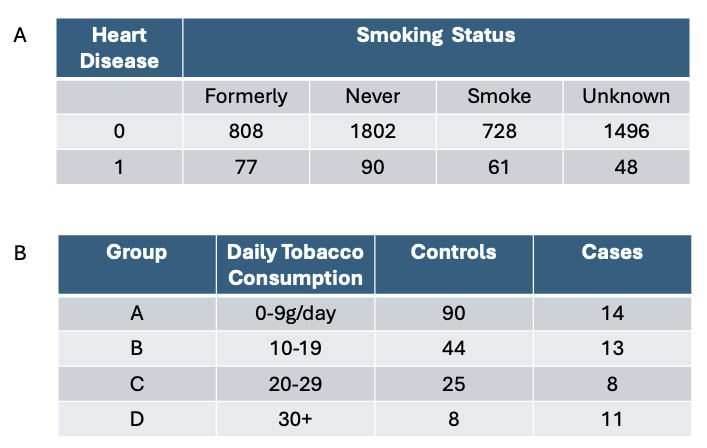
\includegraphics[keepaspectratio]{images/Figure_4-1-SummaryTable.png}}

}

\caption{Recreate summary tables.}

\end{figure}%

Here you will create the two tables in R as shown in Figure
(@ref(fig:Fig4-1)). Let us begin with the first table, which consists of
four columns and two rows. As all the values are numeric, you can create
a numeric vector for each row using the combine or collate function
\texttt{c()} (@ref(vector). But in here, you will specify the vectors a
bit differently. To include the column names in the final table, you
have to associate a name to each value for the first row. For the
subsequent rows, make sure the order of the values corresponds to the
intended columns. As a result, each column in the final table will have
a name when rows are combined. Below is the R code to create two rows
with names using a vector:

\begin{Shaded}
\begin{Highlighting}[]
\NormalTok{row1 }\OtherTok{\textless{}{-}} \FunctionTok{c}\NormalTok{(}\AttributeTok{heart\_disease=}\DecValTok{0}\NormalTok{, }\AttributeTok{formerly=}\DecValTok{808}\NormalTok{, }\AttributeTok{never=}\DecValTok{1802}\NormalTok{, }\AttributeTok{smoke=}\DecValTok{728}\NormalTok{, }\AttributeTok{unknown=}\DecValTok{1496}\NormalTok{)}
\NormalTok{row2 }\OtherTok{\textless{}{-}} \FunctionTok{c}\NormalTok{(}\DecValTok{1}\NormalTok{, }\DecValTok{77}\NormalTok{, }\DecValTok{90}\NormalTok{, }\DecValTok{61}\NormalTok{, }\DecValTok{48}\NormalTok{)}
\end{Highlighting}
\end{Shaded}

Next, you create a table by stacking up the rows using the
\texttt{rbind()} function as shown below.

\begin{Shaded}
\begin{Highlighting}[]
\NormalTok{my\_tab1 }\OtherTok{\textless{}{-}} \FunctionTok{rbind}\NormalTok{(row1, row2)}
\NormalTok{my\_tab1}
\end{Highlighting}
\end{Shaded}

\begin{verbatim}
     heart_disease formerly never smoke unknown
row1             0      808  1802   728    1496
row2             1       77    90    61      48
\end{verbatim}

For example, you can plot the data, perform a \(\chi^{2}\) test of
independence, etc.

\begin{Shaded}
\begin{Highlighting}[]
\FunctionTok{barplot}\NormalTok{(my\_tab1, }\AttributeTok{main=}\StringTok{"Recreate a Table"}\NormalTok{, }\AttributeTok{beside=}\NormalTok{T, }\AttributeTok{legend.text =} \FunctionTok{c}\NormalTok{(}\StringTok{"No heart disease"}\NormalTok{,}\StringTok{"heart disease"}\NormalTok{))}
\end{Highlighting}
\end{Shaded}

\pandocbounded{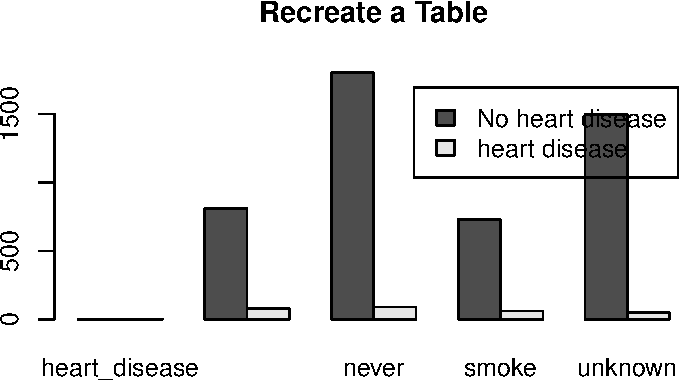
\includegraphics[keepaspectratio]{05_Dive_Deeper_files/figure-pdf/unnamed-chunk-4-1.pdf}}

\begin{Shaded}
\begin{Highlighting}[]
\FunctionTok{chisq.test}\NormalTok{(my\_tab1)}
\end{Highlighting}
\end{Shaded}

\begin{verbatim}
Warning in chisq.test(my_tab1): Chi-squared approximation may be incorrect
\end{verbatim}

\begin{verbatim}

    Pearson's Chi-squared test

data:  my_tab1
X-squared = 61.967, df = 4, p-value = 1.119e-12
\end{verbatim}

For the second table, each row contains a mixture of character and
numeric values. Therefore, vector objects cannot be used to represent
rows @ref(atomic-and-object-variables). Instead, use \texttt{list}
objects for the \textbf{heterogeneous} rows. Below is an example to
define rows as list objects:

\begin{Shaded}
\begin{Highlighting}[]
\NormalTok{A }\OtherTok{\textless{}{-}} \FunctionTok{list}\NormalTok{(}\AttributeTok{group=}\StringTok{"A"}\NormalTok{, }\AttributeTok{daily\_toba=}\StringTok{"0{-}9"}\NormalTok{, }\AttributeTok{ncontrols=}\DecValTok{90}\NormalTok{, }\AttributeTok{ncases=}\DecValTok{14}\NormalTok{)}
\NormalTok{B }\OtherTok{\textless{}{-}} \FunctionTok{list}\NormalTok{(}\StringTok{"B"}\NormalTok{, }\StringTok{"10{-}19"}\NormalTok{, }\DecValTok{44}\NormalTok{, }\DecValTok{13}\NormalTok{)}
\NormalTok{C }\OtherTok{\textless{}{-}} \FunctionTok{list}\NormalTok{(}\StringTok{"C"}\NormalTok{, }\StringTok{"20{-}29"}\NormalTok{, }\DecValTok{25}\NormalTok{, }\DecValTok{8}\NormalTok{)}
\NormalTok{D }\OtherTok{\textless{}{-}} \FunctionTok{list}\NormalTok{(}\StringTok{"D"}\NormalTok{, }\StringTok{"30+"}\NormalTok{, }\DecValTok{8}\NormalTok{, }\DecValTok{11}\NormalTok{)}
\end{Highlighting}
\end{Shaded}

Similarly, rows as lists are stacked up together to form a table.

\begin{Shaded}
\begin{Highlighting}[]
\NormalTok{my\_tab2 }\OtherTok{\textless{}{-}} \FunctionTok{rbind}\NormalTok{(A,B,C,D)}
\NormalTok{my\_tab2}
\end{Highlighting}
\end{Shaded}

\begin{verbatim}
  group daily_toba ncontrols ncases
A "A"   "0-9"      90        14    
B "B"   "10-19"    44        13    
C "C"   "20-29"    25        8     
D "D"   "30+"      8         11    
\end{verbatim}

\section{Create a small data frame with data in
R}\label{create-a-small-data-frame-with-data-in-r}

In this section, you will learn two approaches to store a small dataset
in an R's \texttt{data.frame} object. If you have a large dataset, this
approach might not be the best choice. Instead, you should prepare the
dataset using a spreadsheet software, e.g., Google Sheets or Microsoft
Excel. Read the next section for more details.

\subsection{\texorpdfstring{Use \texttt{data.frame()}
Function}{Use data.frame() Function}}\label{use-data.frame-function}

Besides reproducing a table, you might want to create a small dataset as
a data frame in R. It can be done in two steps, like creating a table
above. The first step is to define each column (variable) as a vector,
and then use the \texttt{data.frame()} function to combine them into a
data frame. Here is an example to create a data frame that consists of
two columns (group, and systolic blood pressure (sbp)), where each
column contains eight samples. The first step is to create two vectors,
one for each column

\begin{Shaded}
\begin{Highlighting}[]
\NormalTok{group\_data }\OtherTok{\textless{}{-}} \FunctionTok{c}\NormalTok{(}\StringTok{"A"}\NormalTok{,}\StringTok{"A"}\NormalTok{,}\StringTok{"A"}\NormalTok{,}\StringTok{"A"}\NormalTok{,}\StringTok{"A"}\NormalTok{,}\StringTok{"B"}\NormalTok{,}\StringTok{"B"}\NormalTok{,}\StringTok{"B"}\NormalTok{)}
\NormalTok{sbp\_data }\OtherTok{\textless{}{-}} \FunctionTok{c}\NormalTok{(}\DecValTok{120}\NormalTok{,}\DecValTok{135}\NormalTok{,}\DecValTok{133}\NormalTok{,}\DecValTok{128}\NormalTok{,}\DecValTok{130}\NormalTok{,}\DecValTok{150}\NormalTok{,}\DecValTok{160}\NormalTok{,}\DecValTok{158}\NormalTok{)}
\end{Highlighting}
\end{Shaded}

Next, use the \texttt{data.frame()} function to combine the vectors into
a data frame.

\begin{Shaded}
\begin{Highlighting}[]
\NormalTok{small\_df1 }\OtherTok{\textless{}{-}} \FunctionTok{data.frame}\NormalTok{(}\AttributeTok{group =}\NormalTok{ group\_data,}
                       \AttributeTok{sbp =}\NormalTok{ sbp\_data)}
\NormalTok{small\_df1}
\end{Highlighting}
\end{Shaded}

\begin{verbatim}
  group sbp
1     A 120
2     A 135
3     A 133
4     A 128
5     A 130
6     B 150
7     B 160
8     B 158
\end{verbatim}

\subsection{\texorpdfstring{Use \texttt{read.table()}
Function}{Use read.table() Function}}\label{use-read.table-function}

An equivalent approach is to type out the values in columns as the
example below, and feed it to the \texttt{read.table()} function through
the \texttt{text=} parameter.

\begin{Shaded}
\begin{Highlighting}[]
\NormalTok{content }\OtherTok{=}\NormalTok{ (}\StringTok{"}
\StringTok{group sbp}
\StringTok{A 120}
\StringTok{A 135}
\StringTok{A 133}
\StringTok{A 128}
\StringTok{A 130}
\StringTok{B 150}
\StringTok{B 160}
\StringTok{B 158}
\StringTok{"}\NormalTok{)}

\NormalTok{small\_df2 }\OtherTok{\textless{}{-}} \FunctionTok{read.table}\NormalTok{(}\AttributeTok{text =}\NormalTok{ content, }\AttributeTok{header =} \ConstantTok{TRUE}\NormalTok{)}
\NormalTok{small\_df2}
\end{Highlighting}
\end{Shaded}

\begin{verbatim}
  group sbp
1     A 120
2     A 135
3     A 133
4     A 128
5     A 130
6     B 150
7     B 160
8     B 158
\end{verbatim}

\section{Load datasets into R}\label{load-datasets-into-r}

In this section, you will learn several ways to load a data file into R.
Data files are usually in two formats: comma-separated (\texttt{.csv})
or tab-separated (\texttt{.txt} or \texttt{.tsv}). In a \texttt{.csv}
file, comma (\texttt{,}) is used as the separator to separate data in
one column from the other column as shown in Figure 4-2A
(@ref(fig:Fig4-2)). The other commonly used separator is the
\texttt{tab} symbol, which is usually invisible, but it is made visible
deliberately in Figure 4-2B.

\begin{figure}[H]

{\centering \pandocbounded{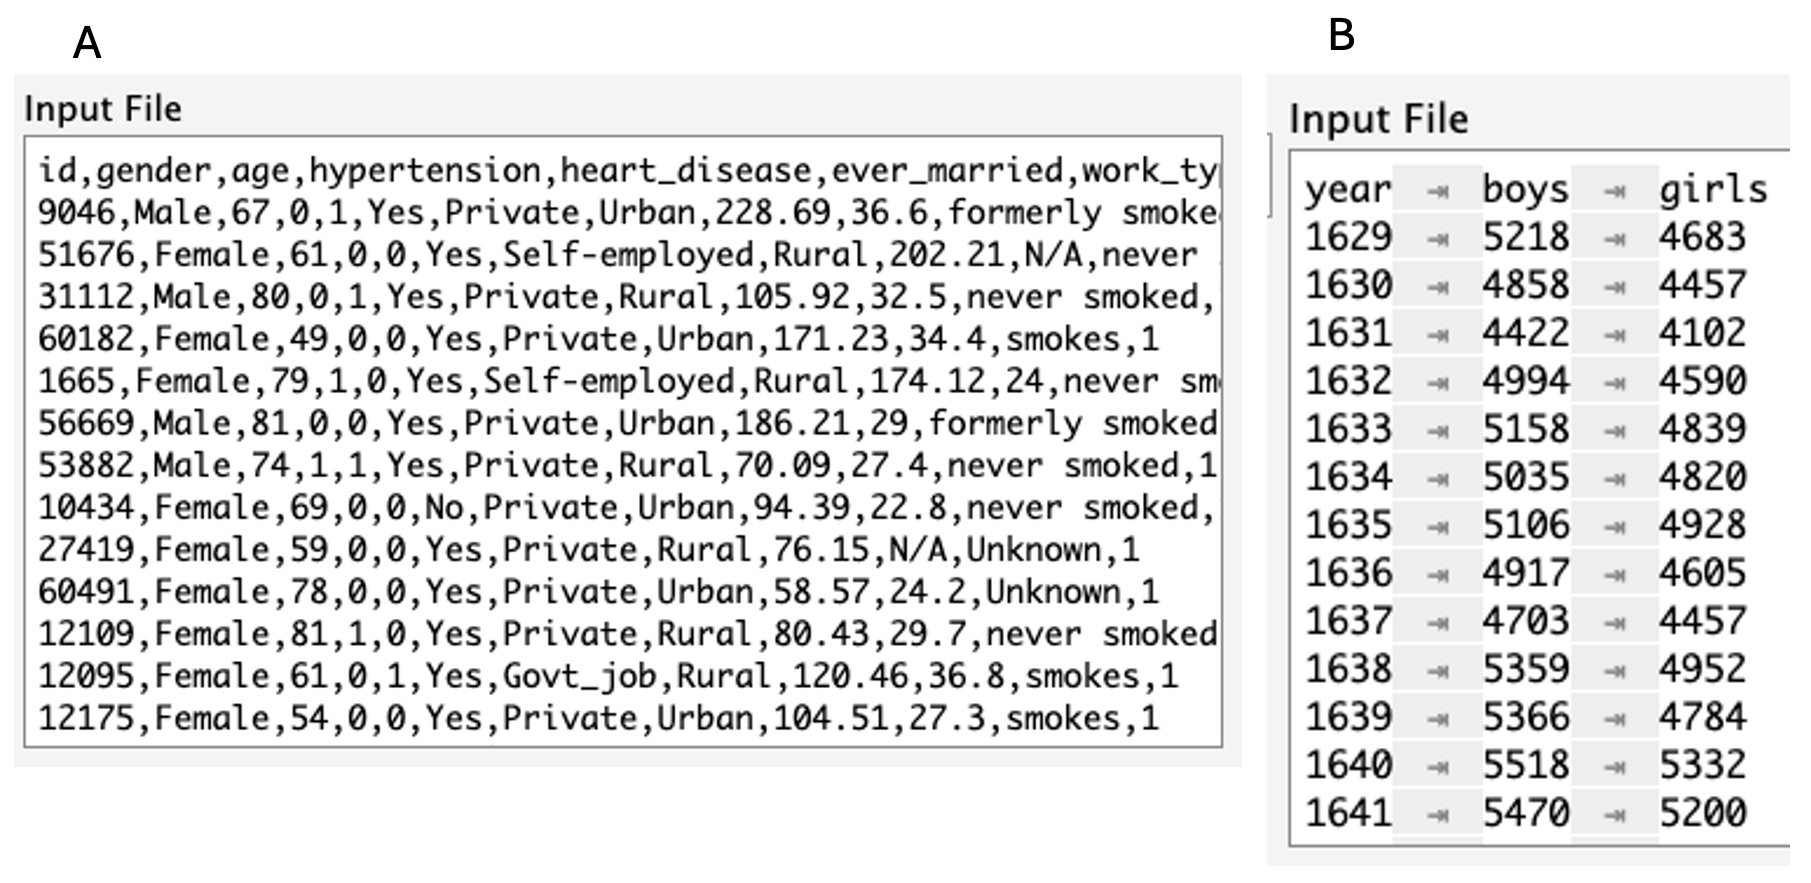
\includegraphics[keepaspectratio]{images/Figure_4-2-FileFormats.png}}

}

\caption{File formats.}

\end{figure}%

\subsection{\texorpdfstring{\texttt{read.csv()}
Function}{read.csv() Function}}\label{read.csv-function}

\subsection{Import data in RStudio}\label{import-data-in-rstudio}

\section{\texorpdfstring{\texttt{group\_by()}}{group\_by()}}\label{group_by}

\section{\texorpdfstring{Different \texttt{apply}
Functions}{Different apply Functions}}\label{different-apply-functions}

\section{Wide to Long}\label{wide-to-long}

Use AirPassengers dataset


\bibliography{book.bib,packages.bib}



\end{document}
